\documentclass[12pt,UTF8,aspectratio=169]{beamer} 
\RequirePackage{mybeamer}
%%% sudo vim /usr/local/texlive/2021/texmf-dist/tex/xelatex/mybeamer
%%%% sudo texhash

\allowdisplaybreaks

%-------------------正文-------------------------%
%                                               %
%                                               %
\begin{document}                                %
%                                               %
%                                               %
%-----------------------------------------------%

%题目,作者,学校,日期                
\author{\myfont 李小飞}
\title{\textbf{\Huge 量子力学与统计物理}}
\subtitle{Quantum mechanics and statistical physics}
\institute[电子科技大学]{{\large 光电科学与工程学院}}
\date{\today}

	%%%%%%%%%%%%%%%%%%%%%%%%%%%%%%%%%
    \frame[plain]{\titlepage}
    %%%%%%%%%%%%%%%%%%%%%%%%%%%%%%%%%
   \begin{frame}
        \frametitle{目录}
        \tableofcontents
    \end{frame}
   %%%%%%%%%%%%%%%%%%%%%%%%%%%%%%%%%%

%\maketitle

%------------------- 章节-------------------------%
%\section{课程简介}

\begin{frame}
  \begin{algorithm}[H]
    \SetAlgoLined
    \KwData{this text}
    \KwResult{how to write algorithm with \LaTeX2e }
    initialization\;
    \While{not at end of this document}{
        read current\;
        \eIf{understand}{
            go to next section\;
            current section becomes this one\;
            }{
            go back to the beginning of current section\;
        }
    }
\caption{How to write algorithms}
\end{algorithm}

\end{frame}

\begin{frame}
  \begin{proof}
    This is a proof
  \end{proof}

\end{frame}

\begin{frame}
  \tcbset{colback=white,arc=0mm,width=(\linewidth-4pt)/4,
  equal height group=AT,before=,after=\hfill,fonttitle=\bfseries}
  
  \noindent
  \foreach \n in {xxx,ggg,AAA,\"Agypten}
  {\begin{tcolorbox}[title=\n,colframe=red!75!black]
    Some content.\end{tcolorbox}}
  
  \noindent
  \foreach \n in {xxx,ggg,AAA,\"Agypten}
  {\begin{tcolorbox}[adjusted title=\n,colframe=blue!75!black]
  Some content.\end{tcolorbox}}
  
  \begin{tcbitemize}[raster columns=3,raster equal height,
            colframe=red!75!black,colback=red!5!white,fonttitle=\bfseries]
  \tcbitem[squeezed title={Short title}]
  First box
  \tcbitem[squeezed title={This is a very very long title}]
  Second box
  \tcbitem[squeezed title={This title is clearly to long for this application}] Third box
  \end{tcbitemize}
  
  \begin{tcbitemize}[raster columns=3,raster equal height,
            colframe=blue!75!black,colback=red!5!white,fonttitle=\bfseries]
  \tcbitem[squeezed title*={Short title}]
  First box
  \tcbitem[squeezed title*={This is a very very long title}]
  Second box
  \tcbitem[squeezed title*={This title is clearly to long for this application}] Third box
  \end{tcbitemize}
\end{frame}


\begin{frame}
  \begin{tcolorbox1}{title}
    This is tcolorbox1
  \end{tcolorbox1}
  \begin{tcolorbox1}[2]{title}
    This is tcolorbox1
  \end{tcolorbox1}
  \begin{tcolorbox2}{title}
    This is tcolorbox2
  \end{tcolorbox2}
  \begin{tcolorbox}{title}
    This is tcolorbox
  \end{tcolorbox}
\end{frame}
                   %
%                                               %
%

\section{1.课程简介}

\begin{frame}
    \frametitle{课程内容}
        \begin{enumerate}
            \Item Fundamentals of quantum informatics(2学时)
            \IItem Fundamentals of quantum mechanics(2学时)
            \Item Quantum information processing and computing(8学时)
            \Item Quantum communication(8学时)
        \end{enumerate}
\end{frame}
\begin{frame} 
    \frametitle{分数构成}
        \begin{enumerate}
            \Item Normal results 20\%
            \Item Group discussion 30\%
            \Item Project final report 60\%
        \end{enumerate}
\end{frame}

\begin{frame}
    \frametitle{参考书目}
        \begin{itemize}
            \Item 《量子计算与量子信息》 (10周年版)  [美]Michael A. Nielsen,Isaac L. Chuang,清华大学出版社,2015        
            \Item 《量子信息处理技术》,赵生妹,郑宝玉,北京邮电大学出版社,2010
            \Item 《Quantum Computation and Quantum Information》(10th Anniversary Edition) , M. A. Nielsen, I. L. Chuang,Cambridge University Press,2011
            \Item 《Quantum Information, Computation and Communication》J. A. Jones,D. Jaksch,Oxford  University Press, 2012
            \Item 《量子信息物理原理》,科学出版社,张永德,   2016
        \end{itemize}
\end{frame}

\begin{frame}
    \begin{tcolorbox4}[分组讨论及报告专题设置(1)]    
        \begin{enumerate}
            \Item   量子叠加态的基本特性及其在量子信息处理中的应用;
            \Item   量子纠缠态的基本特性及其在量子通信中的应用;
            \Item  量子测量的基本特性及其在量子信息学中的应用;
            \Item  信息謪的香农定义和冯诺依曼定义及所带来的影响;
            \Item  量子加法器的量子门及光学线路;
            \Item  量子傅里叶变换的量子线路及光学实现;(明确傅里叶变换的量子基础,明确实现变换的光电器件及线路)
            \Item  质因数量子分解及破获经典密码的量子线路; 
            \Item   单光子、纠缠光子对的产生及检测技术;(该专题应深度结合光电专业知识和技术,明确其在量子信息领域的实际场景) 
        \end{enumerate}
    \end{tcolorbox4} 
\end{frame}

\begin{frame}
    \begin{tcolorbox4}[分组讨论及报告专题设置(2)]    
        \begin{enumerate}
            \Item   量子计算的物理模型与实现;
            \Item   BB84通信协议原理及光学实现;
            \Item   基于纠缠光子对的量子远程传态、量子密钥分配及实现方案;(基于光子技术,理解量子传态的原理,实现的光路及逻辑基础)
            \Item   拉曼散射光学量子中继原理及实现;
            \Item   压缩态的基本特性及其在量子信息学的应用;
            \Item  量子光学通信的研究前沿及最近进展
            \Item  自选专题
        \end{enumerate}
    \end{tcolorbox4} 
\end{frame}

%%%%%%%%%%%%%%%%%%%%%%%%%%%%%%%%%%%55%%
\begin{frame} [plain]
    \frametitle{}
    \Background[1] 
    \begin{center}
    {\huge 第1讲:量子信息与通信基础}
    \end{center}  
    \addtocounter{framenumber}{-1}   
\end{frame}
%%%%%%%%%%%%%%%%%%%%%%%%%%%%%%%%%%

\section{2.量子信息学简介}

\begin{frame} 
    \frametitle{量子信息学定义}
    量子信息学是基于量子力学基本原理对信息进行编码、存储、通信和计算处理的新兴交叉学科。Quantum information: Information that is acquired, processed, or transmitted by a system whose description requires quantum mechanics\\
    \begin{center}
        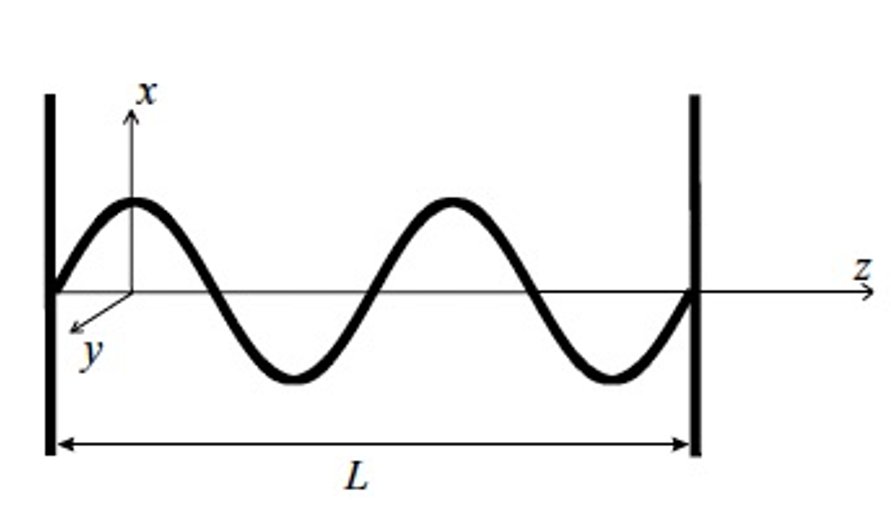
\includegraphics[width=0.55\textwidth]{figs/1.png}
    \end{center}   
\end{frame}

\begin{frame} 
    \frametitle{量子信息学应用}
    \begin{center}
        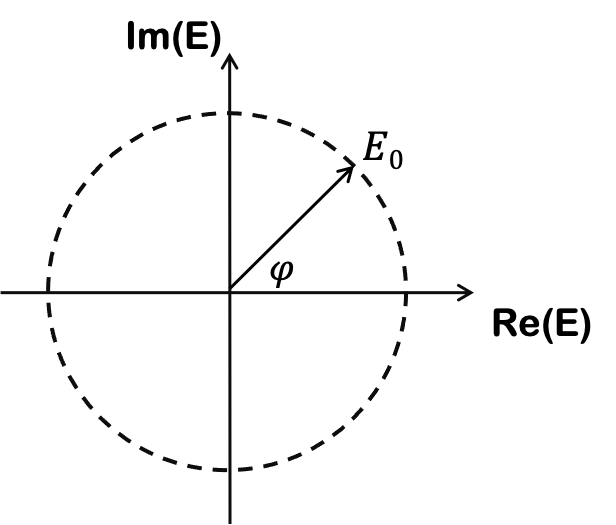
\includegraphics[width=0.7\textwidth]{figs/2.png}
    \end{center}   
\end{frame}

\begin{frame} 
    \frametitle{计算机发展简史}
    \begin{enumerate}
        \Item   算盘 (人力)
        \Item   图灵机(1930)机械,力学
        \Item   电子计算机(1946-1956)电学,真空-电子管,
        \Item   晶体管计算机(1956-1964) 数字,卡片机
        \Item   集成电路(1964-1970)单片机,磁盘,操作系统
        \Item   超大规模集成电路(1970-至今)微处理器
        \Item   量子计算机(...)
    \end{enumerate}
\end{frame}

\begin{frame} 
    \frametitle{Moor's Lore}
    \begin{center}
        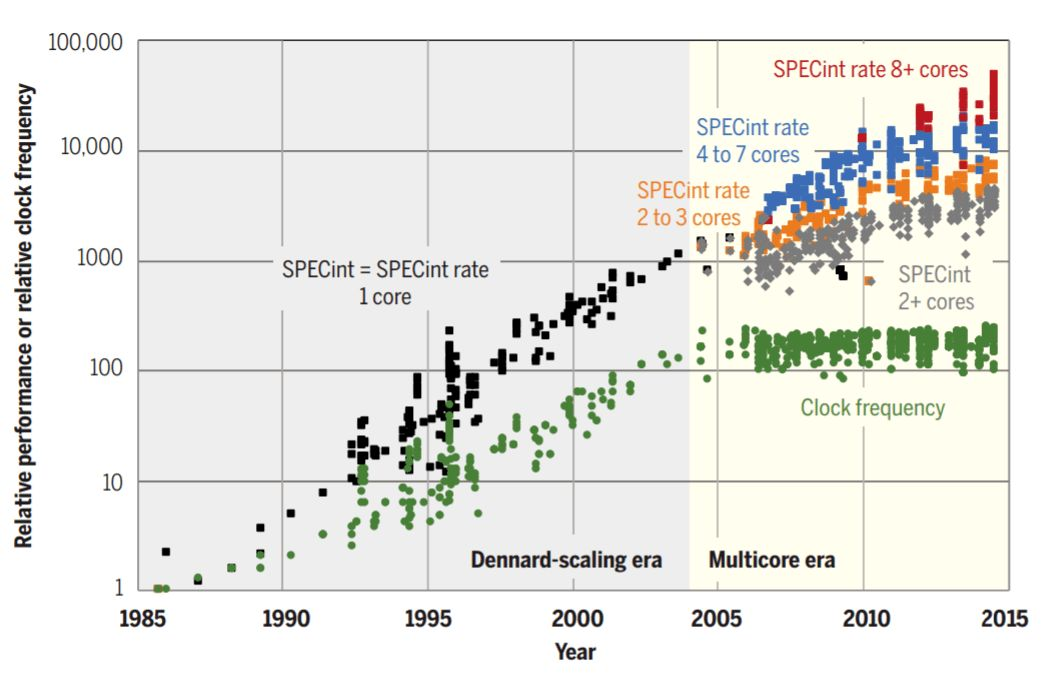
\includegraphics[width=0.8\textwidth]{figs/3.png}
    \end{center} 
\end{frame}

\begin{frame} 
    \frametitle{量子计算机的提出}
    \begin{center}
        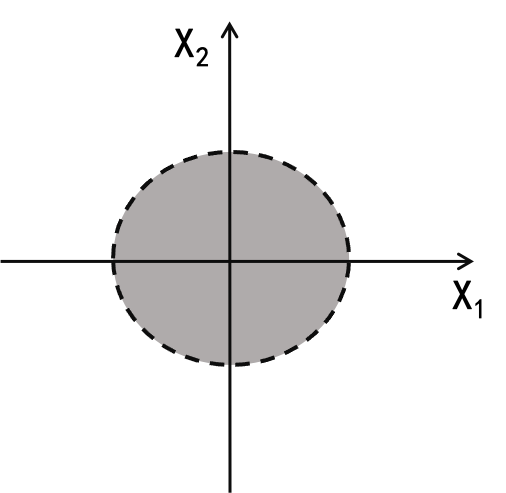
\includegraphics[width=0.8\textwidth]{figs/4.png}
    \end{center} 
\end{frame}

\begin{frame} 
    \frametitle{量子计算实现的难点}
    \begin{enumerate}
        \Item   量子计算机的顶层设计(数学模型)
        \Item   量子信息表示(比特与物理模型)
        \Item   量子态的保持(叠加态消相干)
        \Item   多量子并行(多量子多自由度纠缠)
    \end{enumerate}
\end{frame}

\begin{frame} 
    \frametitle{量子通信实现的难点}
    \begin{enumerate}
        \Item   量子态能传多远
        \Item   量子纠缠能传多远
    \end{enumerate}
    \begin{center}
        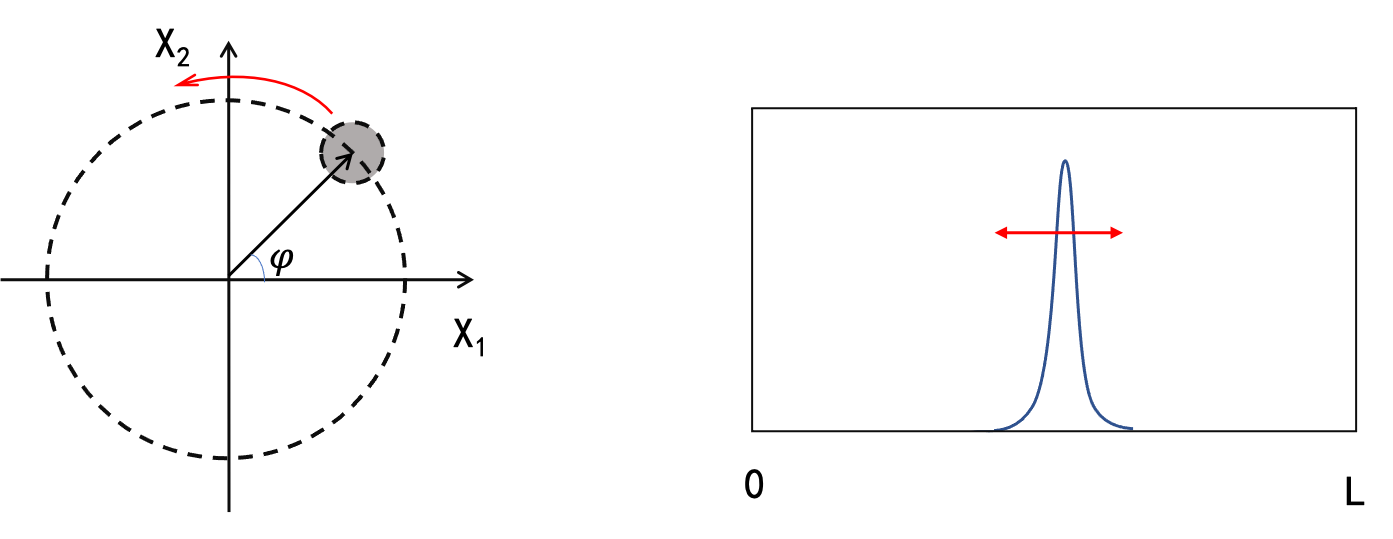
\includegraphics[width=0.8\textwidth]{figs/5.png}
    \end{center} 
\end{frame}

\begin{frame} 
    \frametitle{量子计算发展三阶段}
    \begin{center}
        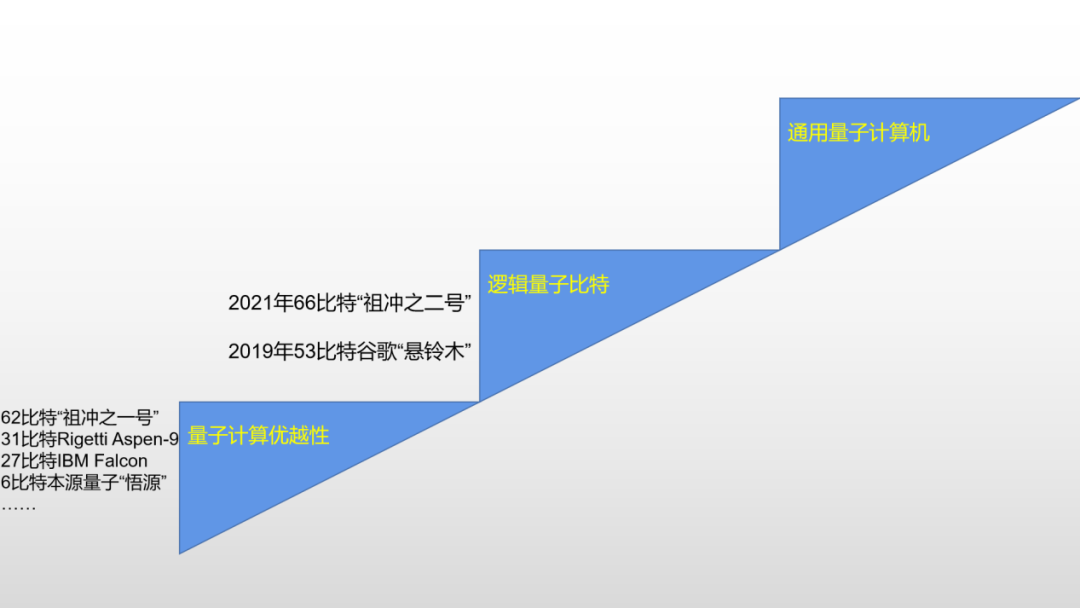
\includegraphics[width=0.9\textwidth]{figs/6.png}
    \end{center} 
\end{frame}

\begin{frame} 
    \frametitle{量子计算公司TOP10}
    \begin{enumerate}
        \Item   Accenture(埃森哲,英)
        \Item   阿里巴巴
        \Item   AT\&T
        \Item   Atos(源讯)
        \Item   百度
        \Item   谷歌
        \Item   IBM
        \Item   Intel
        \Item   微软
    \end{enumerate}
\end{frame}

\section{3.量子比特}

\begin{frame} 
    \frametitle{Bit and Qubit}
    \begin{center}
        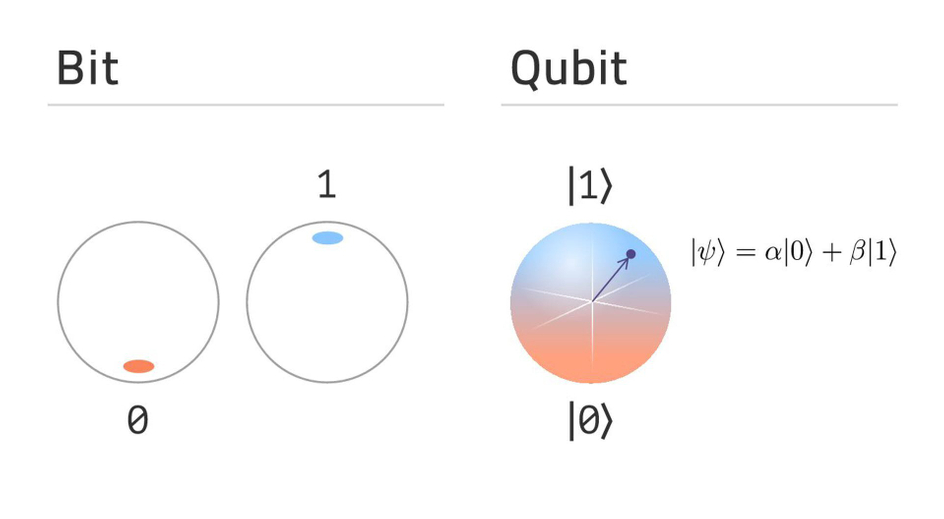
\includegraphics[width=0.8\textwidth]{figs/7.png}
    \end{center} 
\end{frame}

\begin{frame} 
    \frametitle{量子比特的物理实现}
    量子比特在物理上是二能级系统,因此,有以下可能的实现方案\\
    \begin{enumerate}
        \Item   光子
        \Item   电子
        \Item   原子
        \Item   离子色心
        \Item   分子
        \Item   超导材料
        \Item   拓扑材料
    \end{enumerate}
\end{frame}

\begin{frame} 
    \frametitle{量子比特的数学抽象}   
    这两个能态在数学上可抽象为
    \begin{enumerate}
        \Item   $\rs{0}$
        \Item   $\rs{1}$
    \end{enumerate}
    称为两个正交归一的计算基矢态\\
    量子比特可抽象为
    \begin{enumerate}
        \Item   $\rs{\psi} =\alpha\rs{0}+\beta\rs{1}, \qquad (|\alpha|^2+|\beta|^2=1)$
    \end{enumerate}
    \Note~量子比特可处于$\rs{0}$或 $\rs{1}$ 计算基矢态,也可处于它们的叠加态$\rs{\psi}$
\end{frame}

\begin{frame} 
    \frametitle{量子比特的角度表示} 
  由于\[|\alpha|^2+|\beta|^2=1)\]
  叠加态可表示成角度形式  
  \[\begin{aligned}
    \rs{\psi} &=\alpha\rs{0}+\beta\rs{1} \\
    &=e^{i\gamma} \left(\cos\frac{\theta}{2}\rs{0}+e^{i\varphi} \sin\frac{\theta}{2}\rs{1}\right) \\
    &=\cos\frac{\theta}{2}\rs{0}+e^{i\varphi} \sin\frac{\theta}{2}\rs{1}
  \end{aligned}\]
  \Note~量子比特由两个角度$\theta, \varphi$ 确定
\end{frame}

\begin{frame} 
    \frametitle{量子比特的几何表示} 
  在($r,\theta,\varphi$)坐标系中,由于$r\equiv 1$, 量子比特可用Bloch球面描述。此时,$\theta, \varphi$ 确定球面上一个点
  \begin{center}
    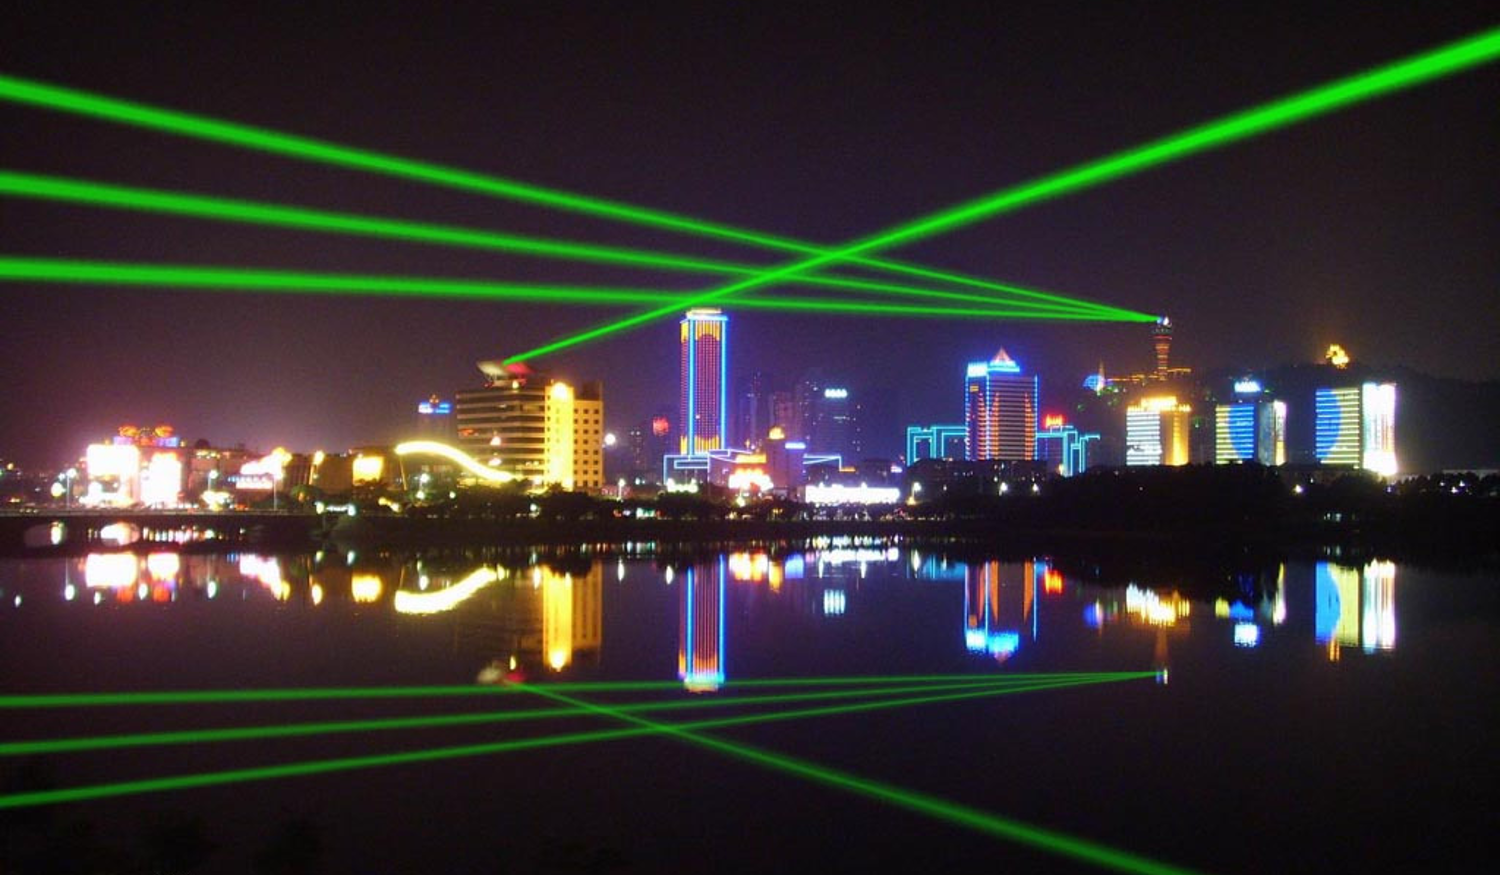
\includegraphics[width=0.4\textwidth]{figs/8.png}
\end{center} 
\end{frame}

\begin{frame} 
    \frametitle{量子比特的矩阵表示}
    \[\rs{\psi} =\alpha\rs{0}+\beta\rs{1} \] 
    态函数与系数矩阵有对应关系\\
   \[
    \begin{matrix} 
    \rs{\psi} =\begin{pmatrix}
            \alpha\\
            \beta
    \end{pmatrix}
    &    
    \rs{0} 
    =\begin{pmatrix}
        1\\
        0
    \end{pmatrix}
    &
    \rs{1} 
    =\begin{pmatrix}
        0\\
        1
    \end{pmatrix}
    \end{matrix}    
    \]
\end{frame}

\begin{frame} 
    \frametitle{量子比特的外积}
    由矩阵表示可知量子比特的外积$\rl{\psi}{\psi}$是一个$2\times 2$的矩阵,
    泡利矩阵是正交归一完全集,
    因此,此外积可在泡利矩阵上展开!
    \[\begin{aligned}
    \rl{\psi}{\psi} 
    &=
    \begin{pmatrix}
        \alpha\\
        \beta
    \end{pmatrix}
    \begin{pmatrix}
        \alpha & \beta
    \end{pmatrix}
 \\
    &= \frac{1}{2}I +\frac{1}{2}\sin\theta\cos\varphi\sigma_x +\frac{1}{2}\sin\theta\sin\varphi\sigma_y+ \frac{1}{2}\cos\theta\sigma_z 
\end{aligned}\]
式中,泡利矩阵为
\[
\sigma_x =
\begin{pmatrix}
    0 & 1 \\
    1 & 0 
\end{pmatrix}, \qquad
\sigma_y =
\begin{pmatrix}
    0 & -i \\
    i & 0 
\end{pmatrix}, \qquad
\sigma_z =
\begin{pmatrix}
    1 & 0 \\
    0 & -1 
\end{pmatrix}
\]
\end{frame}

\section{4.双量子比特}


\begin{frame} 
\frametitle{双量子比特计算基矢态}
两个经典比特有四种状态:\\
00,01, 10, 11\\
(1).两个量子比特有四种计算基矢态:
\[\rs{00}, \qquad \rs{01}, \qquad \rs{01}, \qquad \rs{11} \] 
它们的矩阵表示由原矩阵的直积表示 
\[\rs{01} = \rs{0} \otimes \rs{1} =    
\begin{pmatrix}
    0\\
    1
\end{pmatrix}
\otimes
\begin{pmatrix}
    1\\
    0
\end{pmatrix}
=
\begin{pmatrix}
    0 \otimes \begin{pmatrix}
        1\\
        0
    \end{pmatrix}\\
    1 \otimes \begin{pmatrix}
        1\\
        0
    \end{pmatrix}
\end{pmatrix}
=
\begin{pmatrix}
    0\\
    1\\
    0\\
    0
\end{pmatrix}
 \] 

\end{frame}

\begin{frame} 
\[
\rs{00} = 
\begin{pmatrix}
    1\\
    0\\
    0\\
    0
\end{pmatrix},\qquad
\rs{01} = 
\begin{pmatrix}
    0\\
    1\\
    0\\
    0
\end{pmatrix},\qquad
\rs{10} = 
\begin{pmatrix}
    0\\
    0\\
    1\\
    0
\end{pmatrix},\qquad
\rs{1} = 
\begin{pmatrix}
    0\\
    0\\
    0\\
    1
\end{pmatrix}
\] \vspace{0.6em}
\Note 四个计算基矢态$ \rs{00}, \rs{01},\rs{10},\rs{11} $构成正交归一完全集。
\end{frame}

\begin{frame} 
    \frametitle{双量子比特叠加态}
(2). 双量子比特任意态是四个计算基矢态的叠加态:
 \[\rs{\psi} =\alpha_{00}\rs{00}+\alpha_{01}\rs{01}+\alpha_{10}\rs{10}+\alpha_{11}\rs{11}\]
 归一化条件:
 \[ \sum_{ij=0,1} \alpha_{ij}= 1\]
\end{frame}

\begin{frame} 
    \frametitle{测量后态函数}
(3).若对双量子比特的第一个位进行测量,设测量结果为$\rs{0}$,求测量后体系的状态:
 \[\rs{\psi} =\alpha_{00}\rs{00}+\alpha_{01}\rs{01}+\alpha_{10}\rs{10}+\alpha_{11}\rs{11}\]
 测量导致后两计算基矢态消失,变成了:
 \[\rs{\psi} =\alpha_{00}\rs{00}+\alpha_{01}\rs{01}\]
 求归一化系数,得归一化态函数:
 \[\rs{\psi'} =\frac{\alpha_{00}\rs{00}+\alpha_{01}\rs{01}}{\sqrt{|\alpha_{00}|^2+ |\alpha_{01}|^2}} \]
\end{frame}

\begin{frame} 
    \frametitle{三量子比特}
(4).三量子比特有8个计算基矢态:\\
\[\rs{000}, \qquad \rs{001}, \qquad \rs{010}, \qquad \rs{011} , \qquad \rs{100}, \qquad \rs{101}, \qquad \rs{110}, \qquad \rs{111} \] 
三量子比特任意态是这8个计算基矢态的叠加态:
\[\rs{\psi} =\sum_{ijk=0,1} \alpha_{ijk}\rs{ijk}\] 
\end{frame}

\begin{frame} 
    \frametitle{n量子比特}
(5). n量子比特有$2^n$个计算基矢态:\\
{\Bullet} 当n=500时,计算基矢态的数目比宇宙中的原子数目还在多!\\
{\Bullet} 当n=100时,一台量子计算机可以完成全世界当前所有的计算任务!
\end{frame}

\section{4.量子逻辑门}

\begin{frame} 
    \frametitle{量子比特逻辑门}

{\Bullet} 量子计算由量子线路来完成信息的处理和传输,

{\Bullet} 量子线路主要由量子传输线和量子逻辑门构成,

{\Bullet} 量子逻辑门是进行逻辑运算的基本单元,

{\Bullet} 逻辑运算是一切数值计算的基础,

{\Bullet} 在数学上找到一套普适的量子逻辑门,可完成人类所有的逻辑运算。

{\Bullet} 在物理上实现普适的量子逻辑门,构造出量子计算机

\end{frame}

\begin{frame}
    \includemedia[
    width=1.0\linewidth,height=0.60\linewidth, % 16:9
    activate=pageopen,
    addresource=figs/qubit.mp4,
    flashvars={
    source=figs/qubit.mp4
    &autoPlay=true % start playing on activation
    &loop=true
    }
    ]{}{VPlayer.swf}
\end{frame}

\begin{frame}
    \frametitle{}
    \begin{tcolorbox3}[专题学术讨论-1]
        为什么经典计算机必将发展成为量子计算机?
    \end{tcolorbox3}
\end{frame}
%

%%%%%%%%%%%%%%%%%%%%%%%%%%%%%%%%%%%55%%
\begin{frame} [plain]
    \frametitle{}
    \Background[1] 
    \begin{center}
    {\huge 第2讲:量子力学基础}
    \end{center}  
    \addtocounter{framenumber}{-1}   
\end{frame}
%%%%%%%%%%%%%%%%%%%%%%%%%%%%%%%%%%

\section{1.量子态与希尔伯特空间}

\begin{frame} 
    \frametitle{希尔伯特空间}
    量子态用希尔伯特空间中矢量描述\\
    \begin{equation*}
        \begin{split}
            \text{1、定义加法} \quad  &\xi=\psi+\varphi\\
            &\psi+\varphi=\varphi+\psi \qquad (\text{交换律})\\
            &(\psi+\varphi)+\xi=\psi+(\varphi+\xi) \qquad (\text{结合律})\\
            &\psi+\text{O}= \psi \qquad (\text{零元})\\
            &\psi+\varphi= \text{O} \qquad (\text{逆元})\\
        \end{split}  
    \end{equation*}
\end{frame} 

\begin{frame} 
    \begin{equation*}
        \begin{split}
            \text{2、定义数乘} \quad &\varphi=\psi a\\
            &\psi 1= \psi \qquad (\text{1元})\\
            &(\psi a)b=\psi (ab) \qquad (\text{结合律})\\
            &\psi(a+b)= \psi a+ \psi b \qquad (\text{第一分配律})\\
            &(\psi+\varphi) a= \psi a +\varphi a \qquad (\text{第二分配律})\\
        \end{split}  
    \end{equation*}
\end{frame} 

\begin{frame} 
    \begin{equation*}
        \begin{split}
            \text{3、定义内积} \quad &c=(\psi, \varphi)\\
            &(\psi, \varphi)= (\varphi,\psi)^* \\
            &(\psi, \varphi+\xi)= (\psi, \varphi) + (\psi, \xi)\qquad (\text{分配律})\\
            &(\psi, \varphi a)= (\psi, \varphi )a \\
            &\Rightarrow (\psi a, \varphi )= (\psi, \varphi )a^* \\
            &(\psi,\psi)= c\ge 0\\
        \end{split}  
    \end{equation*}
\end{frame}

\begin{frame} 
    \例 [1. 有定义在$C^n$空间的列矩阵,求内积]
    { \[\psi=
        \begin{pmatrix}
                a_1\\
                a_2\\
                a_3
        \end{pmatrix}, \qquad 
        \varphi =\begin{pmatrix}
            b_1\\
            b_2\\
            b_3
    \end{pmatrix}
     \] 
    }
    \解 ~ \[(\psi, \varphi) = \begin{pmatrix}
        a_1 ^* &
        a_2 ^* &
        a_3 ^*
    \end{pmatrix}
        \begin{pmatrix}
        b_1\\
        b_2\\
        b_3
    \end{pmatrix}
    =a_1 ^* b_1 +a_2 ^* b_2 +a_3 ^* b_3
    =c 
    \]
    ~ \[(\varphi,\psi) = \begin{pmatrix}
        b_1 ^* &
        b_2 ^* &
        b_3 ^*
    \end{pmatrix}
        \begin{pmatrix}
        a_1\\
        a_2\\
        a_3
    \end{pmatrix}
    =b_1 ^* a_1 +b_2 ^* a_2 +b_3 ^* a_3
    =c^* 
    \]
\end{frame} 

\begin{frame} 
    \例 [2. 求定义在x空间的函数的内积]{}

    \解 ~ \[(\psi, \varphi)=\int_a ^b \psi^*(x)  \varphi(x) dx
    =c 
    \]
    ~ \[(\psi, \varphi)=\int_a ^b \varphi^*(x)\psi(x) dx = (\int_a ^b \varphi(x)\psi^*(x) dx) ^* =c^*\]
\end{frame} 

\begin{frame}
    4、定义空间\\
   \begin{itemize}
       \Item 矢量空间:满足加法和数乘两种运算的集合
       \Item 内积空间:满足加法、数乘和内积三种运算的集合
       \Item 希尔伯特空间:  完全的内积空间\\
       ~~ \\
       *完全性:对给定任意小的实数$\varepsilon$,总有数N存在,当m, n>N时,有\\
       $$ (\psi_m -\psi_n, \psi_m -\psi_n )< \varepsilon $$
   \end{itemize} 
   \Tips ~ 量子体系的状态用希尔伯特空间的矢量描述
\end{frame} 

\begin{frame}
    5、几个概念\\
   \begin{itemize}
       \Item 模(方):$|\psi|^2= (\psi, \psi)=c$
       \Item 归一化: $|\psi|^2= (\psi, \psi)=c=1$
       \Item 正交(线性无关)性:  $(\psi, \varphi)=0 $ \\
       \Item 完全集: 有一组线性无关集,如果空间的任意矢量都可以在其上展开,则称它为一个完全集,记为$\{\phi_i\}$ 
       \[\psi=\sum_i a_i \phi_i= \sum_i (\phi_i,\psi) \phi_i\]
       \Item 维度:最小完全集所包含矢量的数目相同,称这个数目为空间的维度
       \Item 正交归一完全集:对于一个n维的完全集,有:\[(\phi_i,\phi_j)=\delta_{ij}, \qquad i,j=1,2,3,\cdots, n \]
       \Item 基与基矢:称一个正交归一完全集为空间的一个基,它所含的矢量称不计算基矢(态)
   \end{itemize} 
\end{frame} 

\begin{frame}
 \Tips~ 同一空间可以有不同的基,\\
 $C^2$空间的一个基:
 \[ \rs{0}\equiv\begin{bmatrix}
     1 \\
     0
 \end{bmatrix}; \qquad \rs{1}\equiv\begin{bmatrix}
    0 \\
    1
\end{bmatrix} \]

$C^2$空间的另一个基:
\[ \rs{+}\equiv\frac{1}{\sqrt{2}}\begin{bmatrix}
    1 \\
    1
\end{bmatrix}; \qquad \rs{-}\equiv\frac{1}{\sqrt{2}}\begin{bmatrix}
   1 \\
   -1
\end{bmatrix} \]

\end{frame} 

\begin{frame} 
    \begin{center}
        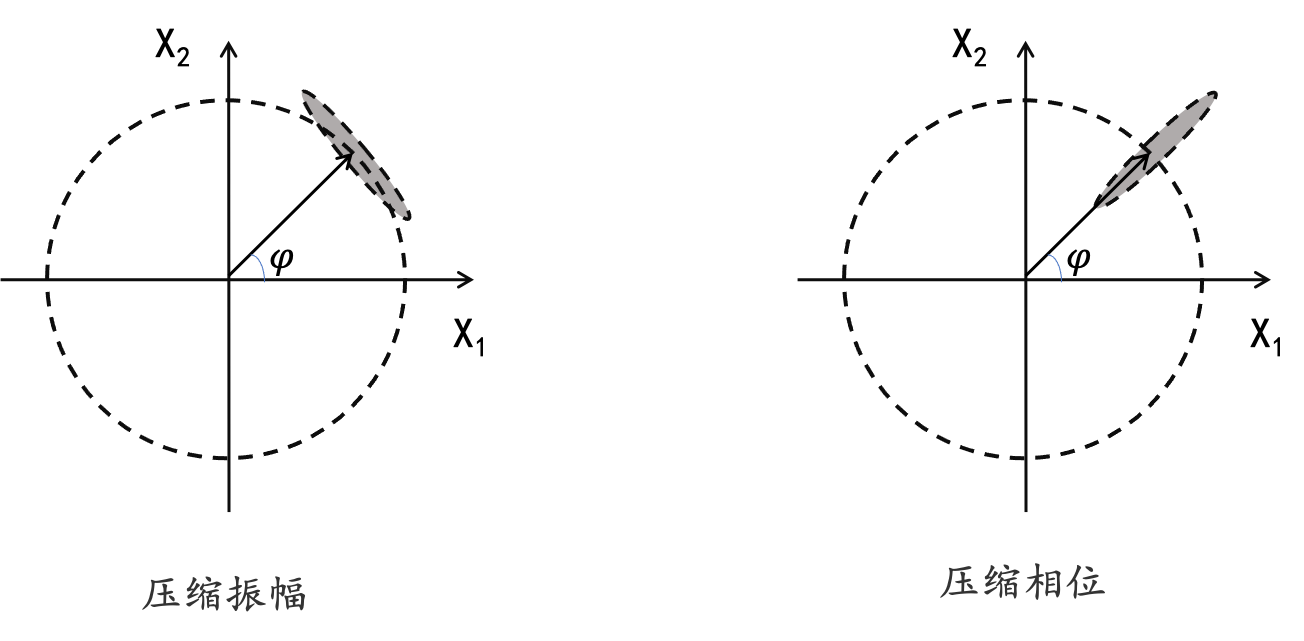
\includegraphics[width=0.4\textwidth]{figs/9.png}
    \end{center} 
\end{frame}


\begin{frame}{}
    6、左矢与右矢\\
    考察内积: $(\psi,\psi)=\int\psi^*\psi d\tau$ \\
    同一波函数放在左边还是右边,意义有所不同: \\
    右边是线性的:  $(\psi,a\psi)=a (\psi,\psi)$ \\
    左边是反线性的:   $(a\psi,\psi)=a^* (\psi,\psi)$  \\
    为了清楚地描述这种线性反线性特点,定义左矢和右矢
    $$\langle \psi |, \qquad |\psi \rangle $$ 
    内积:\[(\psi,\varphi)\equiv \langle \psi | \varphi \rangle\]
    有性质: $$\langle a\psi | = \langle \psi |a^* $$
    $$ |a\psi \rangle = a|\psi \rangle$$ 
\end{frame}

\begin{frame}{}
    7、外积\\
    考察展开式: \[\psi=\sum_i a_i \phi_i= \sum_i (\phi_i,\psi) \phi_i\]
    \[\rs{\psi}=\sum_i a_i \rs{\phi_i}= \sum_i \lr{\phi_i}{\psi} \rs{\phi_i} =\sum_i \rl{\phi_i}{\phi_i} \rs{\psi}\]
    ~~\\
    令 $p_i= \rl{\phi_i}{\phi_i} $, 完备性:
    \[\sum_i p_i= \sum_i \rl{\phi_i}{\phi_i}=1 \]
    称  $p_i= \rl{\phi_i}{\phi_i} $ 外积
\end{frame}

\begin{frame}{}
        \例 [3. 有定义在$C^n$空间的列矩阵,求内积和外积]
        { \[\rs{\psi}=
            \begin{pmatrix}
                    a_1\\
                    a_2\\
                    a_3
            \end{pmatrix}, \qquad 
            \rs{\varphi} =\begin{pmatrix}
                b_1\\
                b_2\\
                b_3
        \end{pmatrix}
         \] 
        }
        \解 ~ \[\lr{\psi}{\varphi} = \begin{pmatrix}
            a_1 ^* &
            a_2 ^* &
            a_3 ^*
        \end{pmatrix}
            \begin{pmatrix}
            b_1\\
            b_2\\
            b_3
        \end{pmatrix}
        =a_1 ^* b_1 +a_2 ^* b_2 +a_3 ^* b_3
        =c 
        \]
        ~ \[\rl{\psi}{\varphi} = \begin{pmatrix}
            a_1  \\
            a_2  \\
            a_3 
        \end{pmatrix}
            \begin{pmatrix}
            b_1 ^* &
            b_2 ^* &
            b_3 ^*
        \end{pmatrix}
        =  \begin{pmatrix}
            a_1b_1 ^* & a_1b_2 ^* & a_1b_3 ^* \\
            a_2b_1 ^* & a_2b_2 ^* & a_2b_3 ^* \\
            a_3b_1 ^* & a_3b_2 ^* & a_3b_3 ^* 
        \end{pmatrix}
        \]
    \Tips ~ 内积是一个数,外积是一个矩阵!
\end{frame}

\section{2.物理量与算符}

\begin{frame}
    \frametitle{算符}
    物理量用希尔伯特空间的线性厄密算符描述\\
    1. 定义:
    \begin{itemize}
        \Item 算符:描述态矢量之间的映射关系,即算符作用于一个态矢量,映射到另一个态矢量。
        \[F \rs{\Psi}=\rs{\psi}\]
        \Item 逆算符  
        \[F^{-1}\rs{\psi}=\rs{\Psi} \] 
        \Item 线性算符 \[F (a\rs{\Psi} +b\rs{\psi}) = aF \rs{\Psi} +bF\rs{\psi}\]
        \Item 伴算符   \[\ls{\psi}=\ls{\Psi}F^{\dagger} \]
    \end{itemize}
\end{frame} 


\begin{frame}
    \frametitle{}
    \begin{itemize}
        \Item 自伴(厄密)算符  \[F = F^{\dagger} \] 性质: $\lr{\Psi F}{\psi}=\lr{\Psi }{F \psi}=\lcr{\Psi }{F} {\psi}$
        \Item 幺正(酉)算符    \[F^{-1} = F^{\dagger} \] 性质: $FF^{\dagger}=F^{\dagger}F=I$, 通常写成 $UU^{\dagger}=U^{\dagger}U=I$ \\
        \Tips 把一个空间所有矢量都用同一幺正算符作用,得到一个新的空间, 即幺正(酉)变换是一种空间变换,
        \[U\rs{\Psi} =\rs{\Psi'}\]
    \end{itemize}
\end{frame} 
\begin{frame}
    \frametitle{}
    \Tips 推导新旧空间算符之间的关系: \\
        旧空间的算符: \[F \rs{\Psi}=\rs{\varphi}\]
        新空间的算符: \[F' \rs{\Psi'}=\rs{\varphi'}\]
        它们之间的关系:
        \[F' U\rs{\Psi}=U\rs{\varphi}\]
        \[F' U\rs{\Psi}=UF \rs{\Psi}\]
        \[U^{\dagger}F' U\rs{\Psi}=U^{\dagger}UF \rs{\Psi}\]
        \[U^{\dagger}F' U\rs{\Psi}=IF \rs{\Psi}\]
        \[U^{\dagger}F' U=F \]
        %\item 
\end{frame}

\begin{frame}
    \frametitle{}
    \begin{itemize}
    \Item 投影算符: 基矢的外积是一种投影算符,
    \end{itemize}
    对于展开式: 
    \[\rs{\psi}=\sum_i a_i \rs{\phi_i}=\sum_i \rl{\phi_i}{\phi_i} \rs{\psi}=\sum_i p_i \rs{\psi} =\sum_i \rs{\psi_i}\]
    有:\[p_i \rs{\psi} =\sum_i \rs{\psi_i}\]
    即,外积$\rl{\phi_i}{\phi_i}$作用于$\rs{\psi}$,得到其在第$i$个基矢态上的投影分量!\\
\end{frame}

\begin{frame}    
    \begin{itemize}
        \Item 测量算子: 量子信息学中常称投影算符为测量算子,定义为
        \end{itemize}
    \[M_0=\rl{0}{0}, \qquad M_1=\rl{1}{1} \]
    具有$2\times 2$的矩阵形式,
    可以证明:\\
    {\bullet} 测量算子是自伴(厄密)算符 :\[M_m = M_m ^{\dagger} \]
    {\bullet} 平方不变性 :\[M_m ^2 = M_m \]
    {\bullet} 完备性 :\[M_0 + M_1 = M_0 ^2 + M_1 ^2 = M_0 M_0 ^\dagger + M_1 M_0 ^\dagger=I\]
\end{frame}

\begin{frame} 
    \frametitle{}
    {\bullet} 测量后的态函数 
    \[\begin{aligned}
        M_0\rs{\Psi} 
        &= \rl{0}{0}(a_0\rs{0}+a_1\rs{1})  \\ 
        &= \rl{0}{0}a_0\rs{0}  \\ 
        &= a_0\rs{0}  \\ 
        &= \frac{a_0}{|a_0|}\rs{0}  \qquad \text{(归一化)} \\ 
    \end{aligned}\]    
    {\bullet} 测得的概率(密度) 
    \[\begin{aligned}
        \lcr{\Psi}{M_0 ^\dagger M_0}{\Psi} 
        &= \lcr{0 }{a_0a_0} {0} \\ 
        &= \lr{0 }{0}a_0 ^* a_0 \\ 
        &= |a_0|^2 = p(0) 
    \end{aligned}\] 
    重写测量后的状态 \[  M_m\rs{\Psi} = \frac{a_m\rs{m}}{\sqrt{\lcr{\Psi}{M_m ^\dagger M_m}{\Psi}}} = \frac{M_m\rs{\Psi}}{\sqrt{\lcr{\Psi}{M_m ^\dagger M_m}{\Psi}}}\]
\end{frame}

\begin{frame}
    \frametitle{}
    \begin{itemize}
    \Item 密度算符: 任意态的外积是一种求概率密度的算符,简称密度算符,
    \end{itemize}
    任意态的展开式:\[\rs{\psi}=\sum_i a_i \rs{\phi_i}\]
    任意态的外积:\[\rho=\rl{\psi}{\psi}\]
    求其在基矢态上的平均值:
    \[\lcr{\phi_i}{\rho}{\phi_i}=\lcr{\phi_i}{\rl{\psi}{\psi}}{\phi_i}=\lr{\phi_i}{\psi}\lr{\psi}{\phi_i}
    =a_i ^* a_i =|a_i|^2=\omega_i     
    \]    
    密度算符的应用,平均值公式-3 
    \[\overline{F}=tr(A\rho)\]
\end{frame}


\begin{frame}
    \frametitle{}
    2. 算符的矩阵表示
    \[\begin{aligned}
        \rs{\psi}&=F \rs{\Psi} \\
        \lr{i}{\psi}&= \lcr{i}{F}{\Psi} \\
        \lr{i}{\psi}&= \sum_j\lcr{i}{F}{j}\lr{j}{\Psi} \\
        \ls{\psi_i}&= \sum_jF_{ij}\rs{\Psi_j} 
    \end{aligned}\]  
    定义了算符矩阵元公式:\[ F_{ij}=\lcr{i}{F}{j}\]
    伴算符的矩阵等于原算符的厄密共轭:\[ F^{\dagger}=(F_{ij} ^*)^T\]
\end{frame}


\begin{frame}
    \frametitle{}
    \例[4.证明平均值公式-3 ]{
    \[\overline{F}=tr(A\rho)\]}
    \证~由矩阵的迹的定义式  
    \[\begin{aligned}
        tr(A\rho) &= \sum_i \lcr{i}{A\rho}{i} \\
        &= \sum_i \lcr{i}{A}{\psi}\lr{\psi}{i} \\
        &= \sum_i \lr{\psi}{i} \lcr{i}{A}{\psi}\\
        &= \lcr{\psi}{A}{\psi}\\
    \end{aligned}\]    
\end{frame}

\begin{frame}
    \frametitle{}
    3. 算符的本征方程
    \begin{itemize}
        \Item 定义式: \[F \rs{\Psi}=f\rs{\Psi}\]
        \Item 相关定理:
        \begin{itemize}
            \IItem 厄密算符的本征值是实数
            \IItem 厄密算符的所有本征矢构成正交归一完全集
            \IItem 当且仅当两厄密算符互相对易时才且有共同的
            本征矢完全集
            \IItem 完全确定一个量子态所需要的彼此对易的一组力学量算符的最小集称为力学量完全集,所含力学量数目与体系的自由度数目相同
            \end{itemize}
    \end{itemize}
\end{frame}

\section{3.张量空间}

\begin{frame}
    \frametitle{张量空间}
    **以上讲的是单粒子体系的量子态及物理量的描述问题
    \begin{tcolorbox4}[张量积]
    {\Bullet}对于多粒子体系,比如多量子比特系统,其所处的空间是子系统希尔伯特空间的张量积。也称直积空间。
    \end{tcolorbox4}
\end{frame}

\begin{frame}
    \frametitle{}
    1. 张量空间的计算基矢 \\
    子系统A是n维的,计算基(某厄密算符的本征函数系)为$$\{\rs{\phi_i}\},\quad (i=1,2,3,\cdots,n)$$ 
    子系统B是m维的,计算基为$$\{\rs{\varphi_j}\},\quad (j=1,2,3,\cdots,m)$$ 
    总系统是n张m维的张量空间,计算基为:$$\{\rs{\phi_i}\otimes\rs{\varphi_j}\},\quad (i=1,2,3,\cdots,n;\quad j=1,2,3,\cdots,m)$$ 
    可简写为:$$\{\rs{\phi_i}\otimes\rs{\varphi_j}\}=\{\rs{\phi_i}\rs{\varphi_j}\}=\{\rs{\phi_i\varphi_j}\}=\{\rs{ij}\}$$
\end{frame}

\begin{frame}
    \frametitle{}
    总体系的任意态是计算基矢的叠加态:
    \[ \rs{\Psi} = \sum_{i,j} a_{ij}\rs{ij}\] \vspace{0.6em}

    \例[写出双量子比特的计算基]{} 
    \解~双量子比特的基由四个计算基矢构成$$\{\rs{00},\rs{01},\rs{10},\rs{11}\}$$
    它们的矩阵形式为:
    \[
\rs{00} = 
\begin{pmatrix}
    1\\
    0\\
    0\\
    0
\end{pmatrix},\qquad
\rs{01} = 
\begin{pmatrix}
    0\\
    1\\
    0\\
    0
\end{pmatrix},\qquad
\rs{10} = 
\begin{pmatrix}
    0\\
    0\\
    1\\
    0
\end{pmatrix},\qquad
\rs{1} = 
\begin{pmatrix}
    0\\
    0\\
    0\\
    1
\end{pmatrix}
\] 
\end{frame}

\begin{frame}
    \frametitle{}
    2. 张量空间的算符 \\
    子系统A有算符$F_A$, 子系统B有算符$F_B$,总系统可定义它们的张量积
    \[F_{AB}=F_A \otimes F_B\]
    作用于总体系的任意态时,算法为:
    \[F_A \otimes F_B \rs{\Psi} = F_A \otimes F_B \sum_{i,j} a_{ij}\rs{ij}=  \sum_{i,j} a_{ij}F_A \rs{i}\otimes F_B\rs{j}\]
    
\end{frame}

\begin{frame}
    \frametitle{}
    3. 子系统的测量与约化密度矩阵 \\
    总体系任意态的密度矩阵
    \[ \rho=\rl{\Psi} {\Psi}= \sum_{i,i',j,j'} a_{i'j'}a_{ij}\rl{i'j'}{ij}\] 
    定义子体系A的约化密度矩阵(把子系统B积分丢!)
    \[ \rho(A)=\sum_{j}\lcr{j}{\rho}{j}=tr_B(\rho)\] 
    测量子体系A的物理量$F_A$的平均值为:
    \[ \bar{F}_A=tr_A(F_A\rho(A))\] 
    
\end{frame}



\section{4.量子力学基本假设}

\begin{frame}
    \frametitle{状态假设}
    \begin{tcolorbox4}[1. 状态假设]
    量子体系的状态用希尔伯特空间的态矢量完全描述。
    \end{tcolorbox4}
    \例[量子比特用2维希尔伯特空间的态矢量]{ 
    \[\rs{\psi} = a_0 \rs{0} + a_1\rs{1}\]完全描述了体系所有可能的状态!}
\end{frame}


\begin{frame}
    \frametitle{演化假设}
    \begin{tcolorbox4}[2. 演化假设]
    一个封闭量子体系的演化用幺正(酉)变换描述。
    \[\rs{\Psi'}=U\rs{\Psi}\]
    状态函数随时间的演化用薛定谔方程描述
    \[ i\hbar \frac{d\rs{\Psi}}{dt}=H \rs{\Psi}\]
    \end{tcolorbox4}
    \例[量子比特]{一套普适量子逻辑门可实现任意幺正(酉)变换
    }
\end{frame}


\begin{frame}
    \frametitle{量子测量假设}
    \begin{tcolorbox4}[3. 量子测量假设]
    量子测量由一组测量算子$\{ M_m\}$ 描述,测得测量值$m$的概率(密度)为
    \[ p(m)=\lcr{\Psi}{M_m ^\dagger M_m}{\Psi} 
     \]
     测量后的状态 \[\frac{M_m\rs{\Psi}}{\sqrt{\lcr{\Psi}{M_m ^\dagger M_m}{\Psi}}}\]
    \end{tcolorbox4}
\end{frame}

\begin{frame}
    \frametitle{张量积假设}
    \begin{tcolorbox4}[4. 复合系统假设]
    复合系统的状态空间是子系统的状态空间的张量积
    \end{tcolorbox4}
\end{frame}

\begin{frame}
    \frametitle{}
    \begin{tcolorbox3}[学术讨论]
        基于以上4个假定,可以从数学上在Hilbert空间导出整个量子力学体系,那么基于假定导出的量子力学可靠吗?
    \end{tcolorbox3}
\end{frame}
%

%%%%%%%%%%%%%%%%%%%%%%%%%%%%%%%%%%%55%%
\begin{frame} [plain]
    \frametitle{}
    \Background[1] 
    \begin{center}
    {\huge 第3讲:量子信息处理-逻辑门}
    \end{center}  
    \addtocounter{framenumber}{-1}   
\end{frame}
%%%%%%%%%%%%%%%%%%%%%%%%%%%%%%%%%%

\section{1.逻辑门的可逆性}

\begin{frame} 
    \frametitle{经典加法器}
    \begin{tcolorbox2}{信息学基本原理}
    所有类型的计算都是加法,二进制加法是逻辑运算,逻辑门是实现各种逻辑运算的基础性元件。
    \end{tcolorbox2}
    \例[1. 设计一个加法器,实现两整数之间的求和]{}
    \解~对于小于$2^n$的正整数$M,N$可表示为:
    \[M=\sum_{i=0} ^{n-1} a_i 2^i,\qquad N=\sum_{i=0} ^{n-1} b_i 2^i\]
\end{frame} 

\begin{frame}    
    \begin{table}
        \caption{加法器真值表,其中 $s_i, c_{i+1}$分别是求和位和进位}
        \begin{tabular}{@{} llll @{}}
          %\toprule
          $a_i$ & $b_i$ & $s_i$ & $c_{i+1}$\\
          \midrule
          0 & 0 & 0 & 0 \\
          0 & 1 & 1 & 0\\
          1 & 0 & 1 & 0\\
          1 & 1 & 0 & 1\\
          \bottomrule
        \end{tabular}
      \end{table}
    \begin{itemize}
        \IItem $a_i$, $b_i$ 不同时, $s_i$置“1”,否则置“0” : 逻辑“异或” XOR  $\qquad s_i=a_i\oplus b_i $
        \IItem $a_i$, $b_i$ 都是1时, $c_{i+1}$置“1”,否则置“0”:   逻辑“与” AND  $\quad c_{i+1}=a_i \wedge b_i $
    \end{itemize}
\end{frame} 

\begin{frame} 
    \frametitle{}
\centering
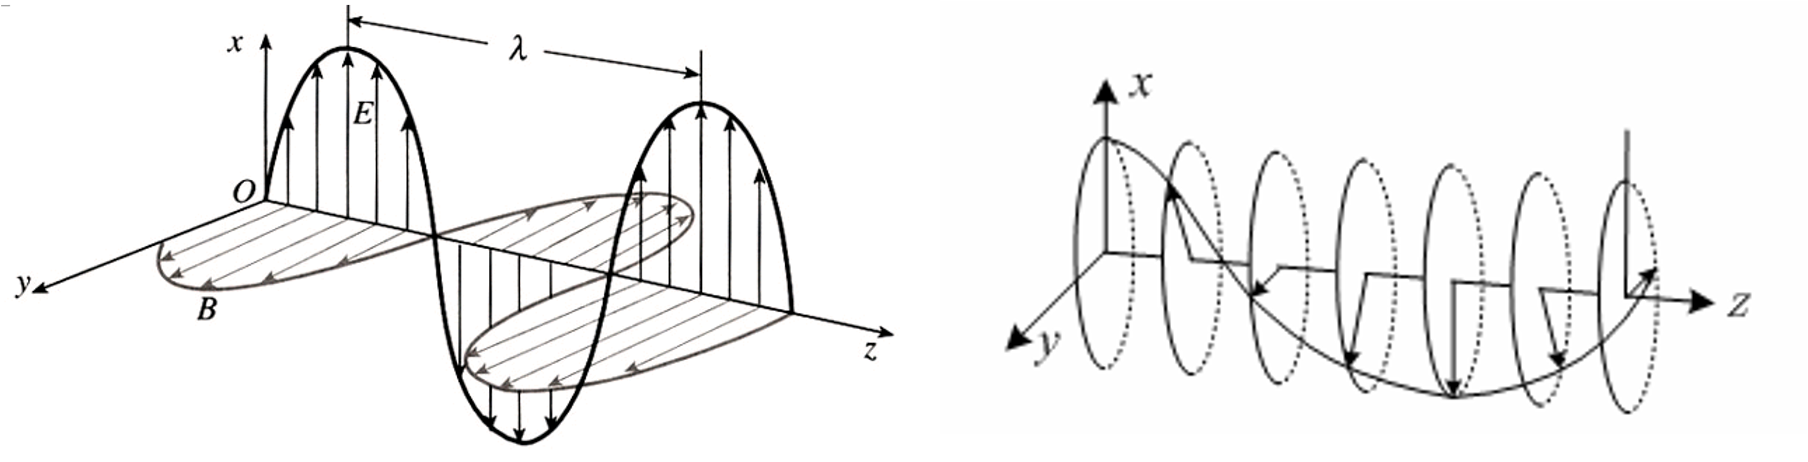
\includegraphics[width=0.45\textwidth]{figs/10.png}
\end{frame} 

\begin{frame} {可逆性}
    考察发现:经典 XOR 门和 AND 门都是不可逆的!\\
    不可逆过程有深刻的物理内含:
    \begin{itemize}
        \IItem 不可逆过程熵增加 $S=k_B\ln\Omega$
        \IItem 不可逆过程信息丢失 $\Delta S=k_B\ln2 $
        \IItem 不可逆过程消耗能量
        \IItem 不可逆过程不是幺正变换
    \end{itemize}
    当前通用的图灵机都是不可逆的! \\ \vspace{0.8em}
    {\Bullet}~~量子计算机通过酉操作(幺正变换)来实现信息处理,要求所有的逻辑门都是可逆的!\\
    
\end{frame}  

\begin{frame} 
    \begin{tcolorbox2}{Bennett 证明}
    所有不可逆的计算机都可以改造为可逆计算机
    \end{tcolorbox2}
    \例[2. 试把不可逆的异或门,改造为可逆的异或门]{}
    \解~改造方法如图 \\
    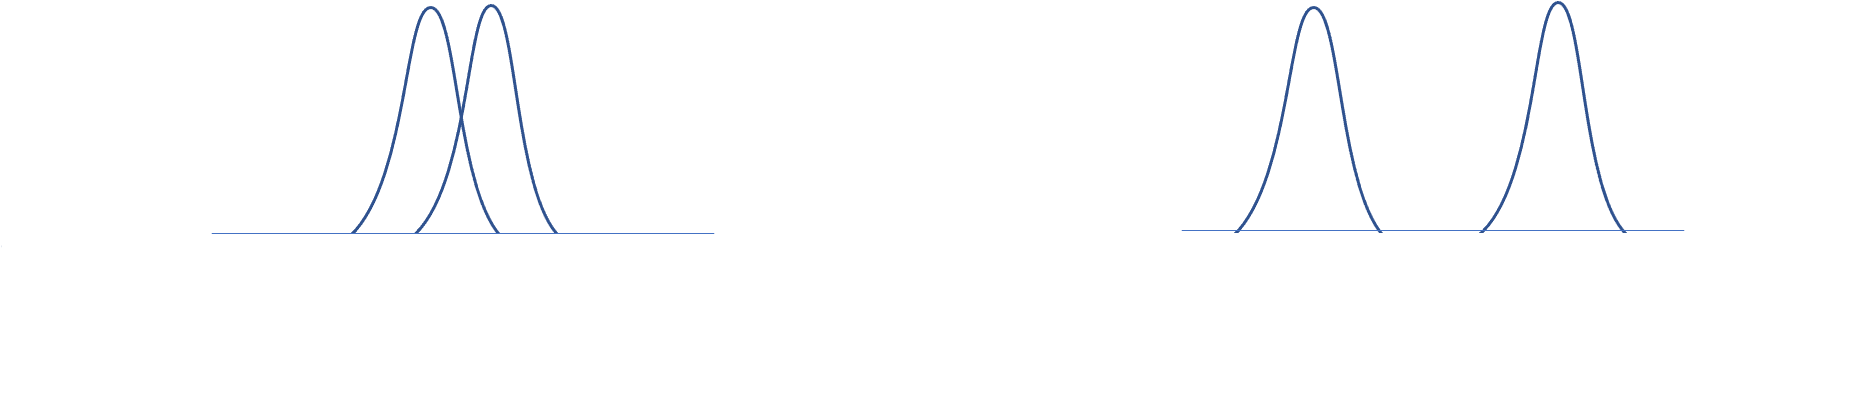
\includegraphics[width=0.7\textwidth]{figs/11.png}
    
    可逆源于所有信息被保留,信息的擦除消耗能量增加熵,导致不可逆。
\end{frame} 



\begin{frame}{}
        \frametitle{麦克斯韦妖佯谬-1871}
        绝热容器分成两格,中间是由“妖”控制的一扇“门”,分子作无规则热运动时会向门上撞击,“门”可以选择性的将速度较快的分子放入一格,
        较慢的分子放入另一格. 这样,体系的熵在减少!\\
       \begin{center}
        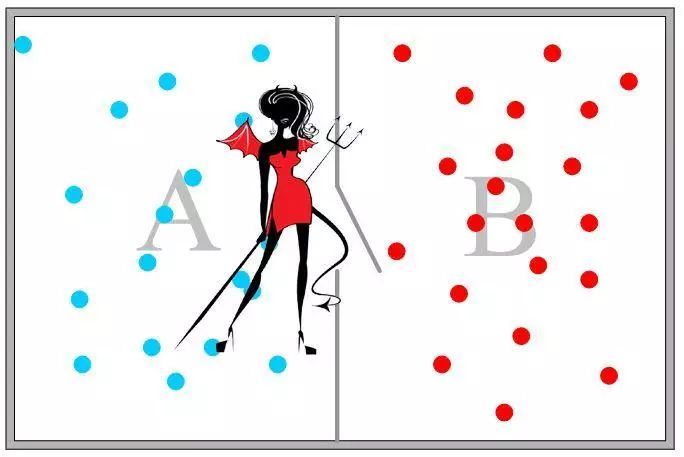
\includegraphics[width=0.42\textwidth]{figs/12.png}     
       \end{center}   
       1981年,Bennett证明“妖”必须去除前面分子的信息,这消耗能量并导致$k_B\ln2$的熵增。 
\end{frame} 

\begin{frame}
    基本结论:\\
   \begin{itemize}
       \IItem 微观过程是可逆的
       \IItem 微观过程服从量子力学原理
       \IItem 演化过程是幺正的
       \IItem 基于幺正变设计的量子逻辑门是可逆的
       \IItem 如果有一套普适的量子逻辑门,发展量子计算机是可行的
   \end{itemize} 
\end{frame} 

\section{2.单量子比特逻辑门}

\begin{frame}
    \frametitle{单量子比特逻辑门}   
单量子比特波函数:
\[\rs{\psi} =\alpha\rs{0}+\beta\rs{1}, \qquad (|\alpha|^2+|\beta|^2=1)\]
矩阵:
 \[ \rs{\psi}=\begin{bmatrix}
    \alpha \\
    \beta
 \end{bmatrix}\]
 因此,单比特逻辑门是操作$C^2$空间的$2\times 2$的矩阵,\\
 由于可逆性的要求,单比特逻辑门也必须是幺正(酉)矩阵。 
\end{frame} 

\begin{frame} 
    \frametitle{1. 量子非门(X-Gate)} 
    经典非门: $0\to 1, \qquad 1 \to 0$ \\
    量子非门: $\alpha\rs{0}+\beta\rs{1} \quad \to \quad\alpha\rs{1}+\beta\rs{0}$ \\ \vspace{1em}

    \例[2. 试证明$\sigma_x$矩阵就是单比特量子非门]
    {~~\\
    \[X \equiv \sigma_x=\XGate = \lr{0}{1}+\lr{1}{0}\]} 
    \证~(1)对于$\rs{\psi} =\alpha\rs{0}+\beta\rs{1}$,有
    \[X \rs{\psi} = X \Qbit{\alpha}{\beta}=\XGate\Qbit{\alpha}{\beta} =\Qbit{\beta}{\alpha}=\beta\rs{0}+\alpha\rs{1}=\alpha\rs{1}+\beta\rs{0}
    \]
\end{frame} 

\begin{frame}     

    (2)幺正性
    \[X^\dagger =(X_{ij} ^*)^T=\XGate\]
    \[X^\dagger X = XX^\dagger =\XGate \XGate=I\]
    证毕!\\ \vspace{1em}
    {\Bullet} 很明显,这是比特反转
    \[ X\rs{0}= \rs{1},\qquad X\rs{1}= \rs{0}
    \]

\end{frame}

\begin{frame}{2.基矢变换门(H-Gate)}
    基矢变换: $\rs{0} \to \rs{+}, \qquad \rs{1} \to \rs{-} $
    \例[4. 试证明如下矩阵就是基矢变换门]
    {~~\\
    \[H \equiv \frac{1}{\sqrt{2}}(X+Z) =\HGate \]} 
    \证~(1)
    \[H \rs{0}= \HGate\Qbit{1}{0}=\frac{1}{\sqrt{2}}\Qbit{1}{1} = \frac{1}{\sqrt{2}}\Qbit{1}{0} +\frac{1}{\sqrt{2}}\Qbit{0}{1} =\frac{\rs{0}+\rs{1}}{\sqrt{2}} =\rs{+}\]
    \[\text{同理}\qquad H \rs{1}=\frac{\rs{0}-\rs{1}}{\sqrt{2}} =\rs{-}\]
\end{frame}

\begin{frame}{}
    (2)幺正性
    \[H^\dagger H = HH^\dagger=I\]
    证毕! \\ \vspace{0.6em}
    \[H \rs{0}=\frac{\rs{0}+\rs{1}}{\sqrt{2}}\]
    \[H \rs{1}=\frac{\rs{0}-\rs{1}}{\sqrt{2}}\]
    {\Bullet} 统一表示为:(x,z 分别取0或1)\\
    \[H \rs{x}=\frac{\sum_z(-1)^{xz}\rs{z}}{\sqrt{2}}\]
\end{frame}

\begin{frame}
    \frametitle{}
    {\Bullet} 可以证明~H 也是自共轭矩阵,有: \[H^\dagger =H \to H^2=I\]
    \例[5. 试证明H可以完成反向变换]
    {~~\\
    \[H \rs{+}= \rs{0}, \qquad H \rs{-}= \rs{1}  \]} 
    \证~ \[H\rs{0}=\rs{+}, \qquad H \rs{0}= \rs{-} \]
    \[HH\rs{0}=H\rs{+} , \qquad H H\rs{0}= H\rs{-}\]
    \[\rs{0}=H\rs{+} , \qquad \rs{0}= H\rs{-}\]
    证毕!
\end{frame}

\begin{frame}
    \frametitle{3. 相位反转门(Z-Gate)} 
    相位反转: $\alpha\rs{0}+\beta\rs{1} \quad \to \quad\alpha\rs{0}-\beta\rs{1}$ \\ \vspace{0.6em}
    \例[3. 试证明$\sigma_z$矩阵就是相位反转门]
    {~~\\
    \[Z \equiv \sigma_z =\ZGate =-i\lr{0}{1}+i\lr{1}{0}\]} 
    \证~(1)
    \[Z \Qbit{\alpha}{\beta}=\ZGate\Qbit{\alpha}{\beta} =\Qbit{\alpha}{-\beta}\]
    (2)幺正性
    \[Z^\dagger Z = ZZ^\dagger=I\]
    证毕!~~ {\Bullet} 很明显~~$ Z\rs{0}=\rs{0},\quad Z\rs{1}=-\rs{1}= e^{i\pi}\rs{1}$
\end{frame}

\begin{frame}
    \frametitle{4. 各种相位门} 
    既然态矢都在 Block球面,那相位反转(Z-Gate)就是绕Z轴旋转180度($\pi$),当然有绕Z轴旋转90度($\dfrac{\pi}{2}$)的门,这就是S-Gate.\\
    \[Z\rs{1}= e^{i\pi}\rs{1}\]
    \[S\rs{1}= e^{i\pi/2}\rs{1}\]
    由此得:\\
    \[S \equiv \SGate = {\begin{bmatrix}
        1 & 0 \\
        0 & e^{\frac{i\pi}{2}}
     \end{bmatrix}}\]
    所以S-Gate=$\sqrt{Z}$-Gate 
\end{frame}
    
\begin{frame}
    当然,也有绕Z轴旋转45度的门,称为T-Gate,也称 $\pi/8$-Gate
    \[S \equiv \SGate = {\begin{bmatrix}
        1 & 0 \\
        0 & e^{\frac{i\pi}{4}}
     \end{bmatrix}}\]
    绕Z轴旋转任意角度($\phi$)的门,则称为旋转门$R_\phi$-Gate
    \[R_\phi \equiv  \RGate \]
    {\Bullet} 很明显~~$ R_\phi\rs{0}=\rs{0},\quad R_\phi\rs{1}= e^{i\phi}\rs{1}$
\end{frame}

\section{3.双量子比特逻辑门}

\section{4.多量子比特逻辑门}

\section{5.普适逻辑门}

\begin{frame}
    \frametitle{}
    \begin{tcolorbox3}[学术讨论]
        基于以上4个假定,可以从数学上在Hilbert空间导出整个量子力学体系,那么基于假定导出的量子力学可靠吗?
    \end{tcolorbox3}
\end{frame}
%
%%%%%%%%%%%%%%%%%%%%%%%%%%%%%%%%%%%%%%%%%%
\begin{frame}
    \frametitle{}
    \begin{center}
    { {\huge 第四讲、态叠加原理}}
    \end{center}    
\end{frame}
%%%%%%%%%%%%%%%%%%%%%%%%%%%%%%%%%%%%%


\section{前情回顾}

\begin{frame}
    \frametitle{前情回顾}
    \begin{itemize}
        \item 波粒二象性
        \item 波函数假说
        \item 波函数的统计解释
    \end{itemize}
\end{frame}  

\section{经典叠加}

\begin{frame}
    \frametitle{经典叠加}
    \begin{center}
        \includegraphics[width=0.5\textwidth]{figs/sup-2.png} \\
    \end{center} 
    依据统计解释,振幅的概率幅\\
    \begin{itemize}
        \item 小球双缝实验,$P'=P_1+P_2 $, 是概率叠加。
        \item 经典叠加是概率叠加!
    \end{itemize}
\end{frame} 

\section{态叠加原理}

\begin{frame}
    \frametitle{态叠加}
    \begin{center}
        \includegraphics[width=0.5\textwidth]{figs/sup-3.png} \\
    \end{center} 
    依据统计解释,振幅的概率幅\\
    \begin{itemize}
        \item 电子双缝实验,$P\neq P_1+P_2 $,不是概率叠加!
        \item 波恩认为服从波函数(态)叠加
        $$ \psi =\psi_1+\psi_2$$
    \end{itemize}
\end{frame} 


\begin{frame} [allowframebreaks=]
    Explanation of the two-slit experiment.\\
    \begin{itemize}
        \item Lets $\psi_1$ describe the state of the electron run across slit-1 and $\psi_2$ for slit-2. \\
        \item when both of them are opened, the electron locates the superposition 
            \[ \Psi=c_1 \psi_1+ c_2\psi_2 \]
        \item the possiblity of electron reaches each point of screen 
    \begin{equation*}
        \begin{split}
            \omega &=|\Psi|^2 \\
            &= (c_1 \psi_1+ c_2\psi_2)^* (c_1 \psi_1+ c_2\psi_2) \\
            &=(\psi_1^*+\psi_2^*)(\psi_1+\psi_2) \\ 
            & = |c_1|^2 |\psi_1|^2 + |c_2|^2 |\psi_2|^2  + [c_1 c_2 ^* \psi_1 \psi_2 ^* + c_1 ^* c_2 \psi_1 ^* \psi_2] \\
        \end{split} 
    \end{equation*}
        \item interference pattern comes from  
     \[[c_1 C_c ^* \psi_1 \psi_2 ^* + c_1 ^* c_2 \psi_1 ^* \psi_2] \]
    \end{itemize}
    \begin{itemize}
        \item 概率计算发现,存在干涉项(后两项),产生干涉条纹。
        \item 电子如果只过一个缝,则$\psi_1$ 或$\psi_2$为零,干涉项为零,没有干涉条纹!
        \item 干涉条纹正是源于电子同时过两个缝, 即电子处于叠加态。
    \end{itemize}
    基于此,波恩提出了态叠加原理
\end{frame}

\begin{frame}
    \frametitle{态叠加原理}
    \begin{tcolorbox1}{Superposition principle of states}
    Born also proposed that: \\
    if $\psi_1$ and $\psi_2$ are the possible states of the system,
    their linear superposition \[ \Psi=c_1 \psi_1+ c_2\psi_2 \]
    is also the possible state of the system.\\
    if the system locates at the superposition $\Psi$, the possiblity of observating the system at $\psi_1$ is $|c_1|^2$, and at $\psi_2$ is $|c_2|^2$ \\
    \[\sum_i |c_i|^2 =1\]
    \end{tcolorbox1}
\end{frame}

\begin{frame}
    \frametitle{}
    \begin{tcolorbox}[colback=yellow!10,colframe=red!75!black,title=态叠加原理]
    如果 $\psi_1$ 、 $\psi_2$、 $\cdots$、$\psi_N$ 是粒子可能的态,那么它们的线性叠加
        $$ \Psi=c_1 \psi_1+ c_2\psi_2+\cdots+c_N\psi_N $$
    也是粒子可能的态(称为叠加态)\\   
    如果粒子处于叠加态 $\Psi=\sum\limits_{i=1}^N c_i \psi_i$,  
    那么测量粒子处在 $\psi_i$ 态的概率为 $\|c_i\|^2$\\ 
    并且  $$\sum_{i=1}^{N} |c_i|^2 =1$$
    \end{tcolorbox}
\end{frame}

\begin{frame}
    \frametitle{实验升级}
    \begin{center}
        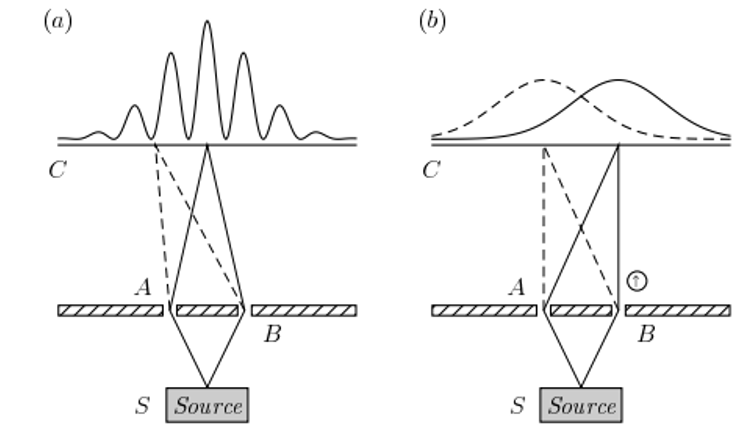
\includegraphics[width=0.5\textwidth]{figs/sup-4.png} \\
    \end{center} 
    \begin{itemize}
        \item 目标:想观测到电子是如何同时过两个缝的
        \item 结果:1)只能测到电子要么过第一缝,要么过第二缝。\\
        2)探测器越灵敏,干涉条纹越模糊,\\
        3) 当探测器能长时间地保持几乎可以完全判断电子过哪条缝时,干涉条纹消失!如图(b)所示
    \end{itemize}
\end{frame}

\begin{frame} [allowframebreaks=]
    \frametitle{结果分析}
    \begin{enumerate}
        \item 测量目的与结果\\
        \begin{itemize}
            \item 当我们“挖出”A和B两条狭缝时,“设计”了一个想要观察“电子的波动性”的设备,也就是电子已经预先被我们设定为“波”,因此我们观测到波动性(干涉条纹)
            \item 当我们装上侦测器时,整个实验被我们“设计”成观察电子的“粒子性”,因为想要知道电子到底是由A还是B穿过时,就必须先具备确定的“位置”的概念,因此我们观察到粒子性(干涉条纹消失)
        \end{itemize}
        \item 测量导致状态发生改变 \\
        \begin{itemize}
            \item 探测前,电子处于叠加态($ \psi =\psi_1+\psi_2$)
            \item 探测时,电子状态改变,被迫从叠加态变变为确定态 ($\psi_1$ or $\psi_2$),称为波函数坍塌
            \item 探测后,电子处于某一单态,不能干涉。
            \item 探测器不灵敏,有部分没有被探测到的电子依然处于叠加态, 干涉条纹模糊。
            \item 探测器灵敏,全部电子被探测,没有电子处于叠加态, 干涉条纹消失。
        \end{itemize}
        \item 测量结果互补(互补性原理)\\
        \begin{itemize}
            \item 波动性和粒子性是两种不同的属性,
            \item 不能因为测得粒子性就否定波动性,反之亦然。
            \item 测量结果就算相互矛盾,也要接受,它们互补地揭示物体的本质。
        \end{itemize}
        \item 结论
        \begin{itemize}
            \item 电子具有波粒二象性,总是处于叠加态
            \item 不被测量,则依然保持在叠加态
            \item 测量导致确定态出来,但结果是随机的。
            \item 测得某个确定态,不能说明电子原本就处于这个态
        \end{itemize}
    \end{enumerate}
\end{frame}

\section{Which Way?}

\begin{frame}
    \frametitle{Which Way?}
    The probabilistic interpretation was controversial from the beginning of of quantum mechanics
    \begin{itemize}
        \item De Broglie : Pilot waves
        \item Schr$\ddot{o}$dinger: Schr$\ddot{o}$dinger's cat
        \item Einstein: EPR paradox
        \item Wheeler's delayed choice experiment
        \item Quantum eraser experiment
        \item $\cdots \cdots$
    \end{itemize}
\end{frame}

\begin{frame}
    \frametitle{薛定谔的猫}
    \begin{center}
        \includegraphics[width=0.8\textwidth]{figs/cat.jpeg} \\
    \end{center} 
\end{frame}

\begin{frame}
    \frametitle{EPR佯谬}
    \begin{center}
        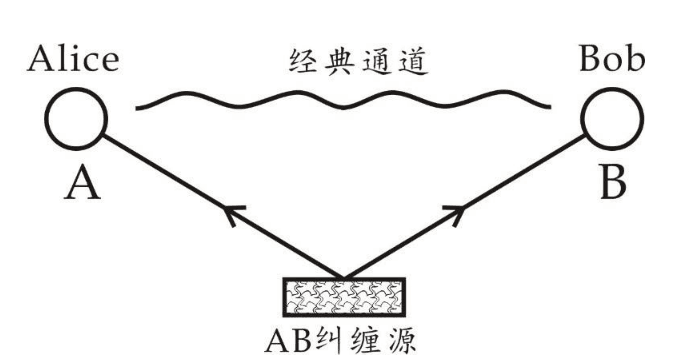
\includegraphics[width=1.0\textwidth]{figs/2022-01-09-14-45-26.png} \\
    \end{center} 
\end{frame}

\begin{frame}
    \frametitle{贝尔不等式}
    \begin{center}
        \includegraphics[width=1.0\textwidth]{figs/bell.png} \\
    \end{center} 
\end{frame}

\begin{frame}
    \frametitle{惠勒延迟选择实验}
    \begin{center}
        \includegraphics[width=0.8\textwidth]{figs/choose.png} \\
    \end{center} 
\end{frame}

\begin{frame}
    \frametitle{量子擦除实验}
    \begin{center}
        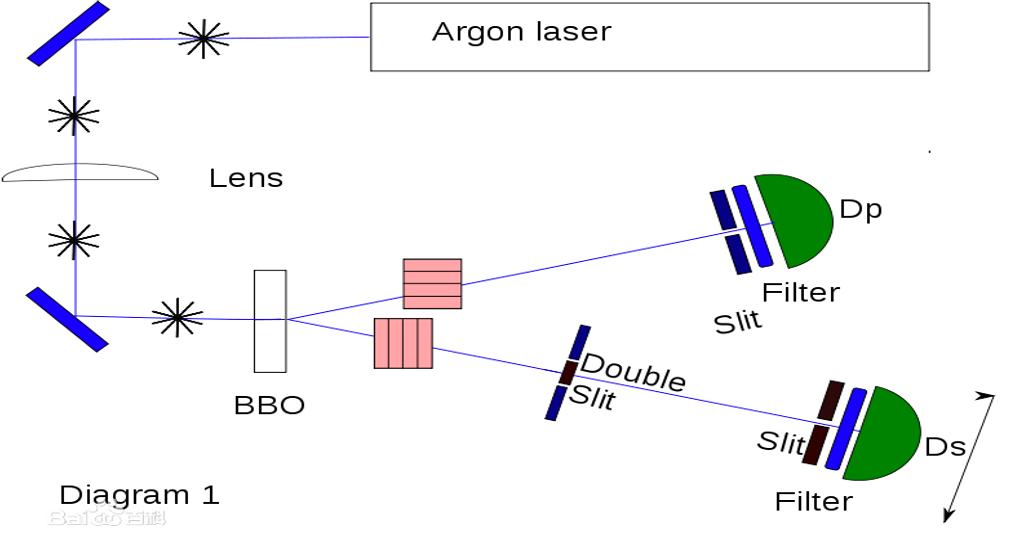
\includegraphics[width=1.0\textwidth]{figs/chachuexp.png} \\
    \end{center} 
\end{frame}

\begin{frame}
    \frametitle{}
    \begin{center}
        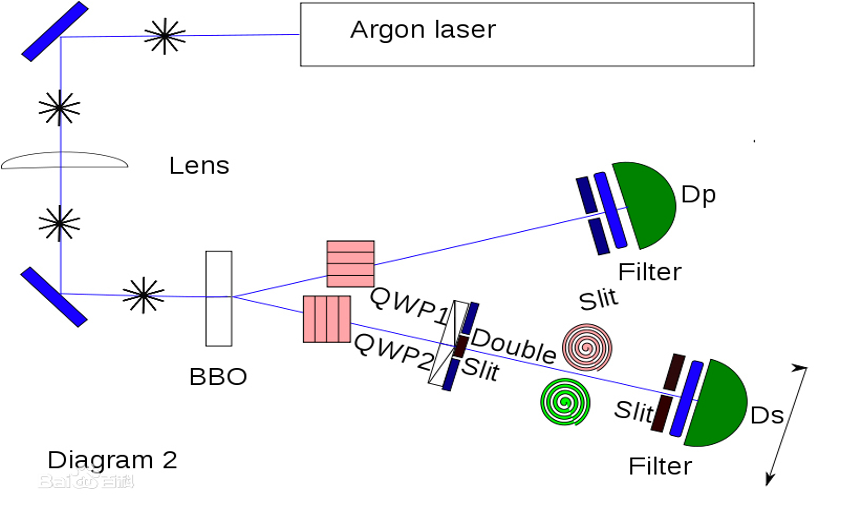
\includegraphics[width=1.0\textwidth]{figs/chachuexp_2.png} \\
    \end{center} 
\end{frame}

\begin{frame}
    \frametitle{}
    \begin{center}
        \includegraphics[width=1.0\textwidth]{figs/chachuexp_3.png} \\
    \end{center} 
\end{frame}

\begin{frame}
    \frametitle{Summary}
    \begin{enumerate}
        \item Objects are wave-particles and can be in states of superposition
        \item Measurement changes the states and gives random results
        \item Measurement results are complementary
        \item Measurement leads to objective reality
    \end{enumerate}
\end{frame}

  
%%%%%%%%%%%%%%%%%%%%%%%%%%%%%%%%%%%%55%%
\begin{frame} [plain]
    \frametitle{}
    \Background[1] 
    \begin{center}
    { {\huge 第五讲、薛定谔方程 }}
    \end{center}  
    \addtocounter{framenumber}{-1}   
\end{frame}
%%%%%%%%%%%%%%%%%%%%%%%%%%%%%%%%%%

%%%%%%%%%%%%%%%%%%%%%%%%%%%%%%%%%
\begin{frame}
        \frametitle{主要内容}
        \transfade
        \tableofcontents
        \addtocounter{framenumber}{-1} 
\end{frame}
%%%%%%%%%%%%%%%%%%%%%%%%%%%%%%%%%%

\section{前情回顾}

\begin{frame}
    \frametitle{前情回顾}
    \begin{itemize}
        \item 波粒二象性
        \item 波函数假说
        \item 波函数统计诠释
        \item 态叠加原理
    \end{itemize}
\end{frame}  

\begin{frame}
    \begin{tcolorbox4}[Conclusion]
        ~~\\
    \begin{enumerate}
        \item Objects are wave-particles and in superposition state
        \item Measurement changes the state and gives random results
        \item Measurement results are complementary
        \item Measurement leads to objective reality
    \end{enumerate}
    \end{tcolorbox4}
\end{frame}  

\begin{frame}
    \tcbbtitle{Big problems}
    \centering
    \tcbb[0.5]
    {
      If not performing measurement, what it would be? 
    }
\end{frame}

\section{薛定谔方程}

\begin{frame}
    \begin{tcolorbox4}[Basic assumption 2/5]
        The evolution of wavefunction obeys Schr$\ddot{o}$dinger equation
        \begin{equation*}
            i\hbar \frac{\partial }{\partial t} \Psi (\overrightarrow{r},t ) =\left [ -\frac{\hbar^2}{2\mu }\nabla ^2 + V(\overrightarrow{r},t ) \right ]\Psi (\overrightarrow{r}, t ) 
        \end{equation*}
    \end{tcolorbox4}
\end{frame}

\begin{frame}
    \frametitle{薛定谔方程}
    \begin{itemize}
        \item 1923年,德布罗意博士论文传到了瑞士,一战炮兵指挥官苏黎世大学讲师薛定谔作了一个关于物质波假说的报告,德拜评注:\\
        $$\text{“有了波,总得有个波动方程吧”}$$
        \item 1926年,薛定谔:
        $$“Dear Debye, I find one \cdots”$$
    \end{itemize}            
\end{frame}

\begin{frame}
    \begin{alertblock} {神秘来源}  
    \begin{quote}
        “是粒子还是波?是妻子还是情人?这都是难题!” \\
        ~~\\
        \rightline{--《薛定谔的女友》(2001)\hspace{6em}}   
    \end{quote}  
    \begin{quote}    
    这部话剧讲述了薛定谔方程建立的神秘过程:在1925年圣诞节前,薛定谔像往年一样,来到阿尔卑斯山度假。这次陪伴他的不是妻子安妮,而是维也纳的一位神秘女郎。
    就是这位比薛定谔的猫还神秘的女郎激发了薛定谔的灵感,使他在一年的时间里连发~6~篇~“SCI”~论文,建立波动量子力学,\ddots\\
    ~~\\
    \end{quote} 
    \end{alertblock}   
\end{frame}

\begin{frame}
	\begin{alertblock} {可能思路}  
		\begin{itemize}
			\item 	\textbf{1:}  最小作用量原理 $\int\limits_{t_1}^{t_2} \delta L d t =0 $\\ 
			\item 	\textbf{2:}  波粒二象性\\ 
			~\\ 
			\item 	\textbf{3:}  不能推导\\
            ~\\ 
            \begin{quote}
            "It is not possible to derive it from anything you know. It came out of the \alert{\faHeartbeat} of Schr$\ddot{o}$dinger"\\
            \rightline{$\cdots$ R. P. Feynman \hspace{3em}}   
            \end{quote}
		\end{itemize}
	\end{alertblock}
\end{frame}

\begin{frame} [allowframebreaks=]
    \frametitle{}
    \alert{\faHeartbeat} Quantum plane wavefunction \[\psi(x,t)=\Psi_p(x,t)=e^{\frac{i}{\hbar}(p\cdot x-Et)} \]
    should be a sulotion of this equation
    \begin{equation*}
        \begin{split}
       -i\hbar \nabla \psi(x,t) &=p\psi(x,t) \\
       \hbar^2 \nabla^2 \psi(x,t) &=p^2\psi(x,t) \\
       \frac{\hbar^2}{2\mu} \nabla^2 \psi(x,t) &=\frac{p^2}{2\mu} \psi(x,t) , \qquad \cdots (1)
        \end{split}
    \end{equation*}
    \begin{equation*}
       i\hbar \frac{\partial }{\partial t} \psi(x,t) =E\psi(x,t)  , \qquad \cdots (2)
     \end{equation*}
    (2)-(1)
    \begin{equation*}
        (i\hbar \frac{\partial }{\partial t} - \frac{\hbar^2}{2\mu} \nabla^2 )\psi(x,t) =(E-\frac{p^2}{2\mu})\psi(x,t)=0  
    \end{equation*}
    \begin{equation*}
        i\hbar \frac{\partial }{\partial t} \psi(x,t) = \frac{\hbar^2}{2\mu} \nabla^2 \psi(x,t)
    \end{equation*}
    For general wavefunction, it's a wave packet of plane wavefunction
    \begin{equation*}
        \Psi(x,t)= \int\limits_{p=0} ^{\infty} c(p,t) e^{\frac{i}{\hbar}px}dp
    \end{equation*}
    we get 
    \begin{equation*}
        \begin{split}
        (i\hbar \frac{\partial }{\partial t} - \frac{\hbar^2}{2\mu} \nabla^2 )\Psi(x,t) &= \int\limits_{p=0} ^{\infty} c(p,t) (E-\frac{p^2}{2\mu}) e^{\frac{i}{\hbar}px}dp=0  \\
        i\hbar \frac{\partial }{\partial t} \Psi(x,t) &= \frac{\hbar^2}{2\mu} \nabla^2 \Psi(x,t)
        \end{split}
    \end{equation*}
    For nonfree particle in a potential $U(x)$,
    \begin{equation*}
        \boxed{i\hbar \frac{\partial }{\partial t} \Psi(x,t) = (\frac{\hbar^2}{2\mu} \nabla^2 +U(x)) \Psi(x,t)}
    \end{equation*}
    That is the Schr$\ddot{o}$dinger equation. \\
    ~~\\
    \bullet For N-particles system
   {\small \begin{equation*}
        i\hbar \frac{\partial }{\partial t} \Psi(x_1, x_2, \cdots x_N,t) = [\sum_{i=1} ^{N} \frac{\hbar ^2}{2\mu_i} \nabla^2 +U(x_1, x_2, \cdots x_N)] \Psi(x_1, x_2, \cdots x_N,t)
    \end{equation*}}
\end{frame}

\begin{frame}
    \frametitle{}
    检验正确性:
    \begin{enumerate}
        \item 自由粒子的解
        \item 氢原子光谱
        \item $\cdots \cdots$
    \end{enumerate}
    ~\\ 
    发表论文:《Quantisierung als Eigenwert problem》(量子化是本征值问题),整整140页!
\end{frame}

\begin{frame}
    \begin{enumerate}
        \item 
        \begin{quote}
            “我一阅读完毕整篇论文,就像被一个迷语困惑多时渴慕知道答案的孩童,现在终于听到了解答!” \\
            ~~\\
            \rightline{--普朗克(1926)\hspace{5em}}   
        \end{quote}  
        \item 
        \begin{quote}
            “这著作的灵感如同泉水般源自一位真正的天才!” \\
            ~~\\
            \rightline{--爱因斯坦(1926)\hspace{4em}}   
        \end{quote}  
        \item  
        \begin{quote}
            “你的方程把量子理论推进了关键性的一步!” \\
            ~~\\
            \rightline{--玻尔(1926)\hspace{6em}}   
        \end{quote} 
    \end{enumerate}
\end{frame}

\begin{frame}
    \frametitle{薛定谔}
    \begin{wrapfigure} {r} {0.3\textwidth} %;图在右
        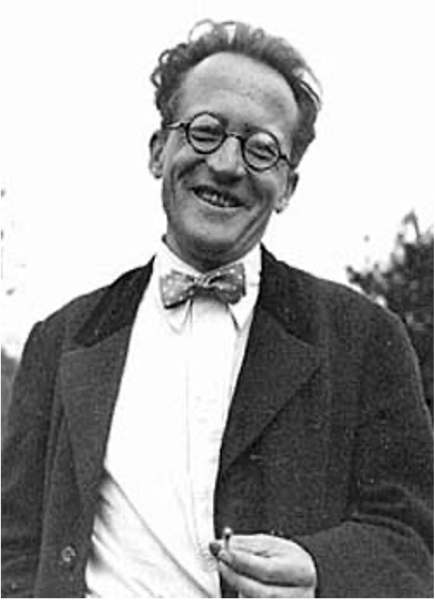
\includegraphics[width=0.25\textwidth]{figs/schroginger.png}   
    \end{wrapfigure}
奥地利理论物理学家, 生于维也纳, 量子力学的奠基人之一。薛天才,通灵的人, 1926年提出薛定谔方程,获1933年诺贝尔物理学奖; 1935年提出“薛定谔的猫”,至今还是“养猫人”的猫王;1943年写的《生命是什么》一书,被誉为“唤起生物革命的小册子”。\\ \vspace{0.3em}
薛定谔:他玉树临风,英俊潇洒,风流倜傥,人见人爱,花见花开,情人无数,江湖人称“段正淳"
\end{frame}

\begin{frame}
    \frametitle{}
    \tcbbtitle{\large Significance }
    \centering
    \tcbb[0.5]
    {
      \large {It's the most fundamental equation in quantum mechanics. 
      It's the starting point for every quantum mechanical system we want to describe: electrons, protons, neutrons, whatever.
      And now, it has become the established analogue of Newton's second law of motion for quantum mechanics}
    }
\end{frame}

\section{定态薛定谔方程}

\begin{frame} 
    \frametitle{定态问题}
    若势函数$V(\vec{r},t ) $若不显含时间 t,则时间变量可分离 \\ \vspace{0.3cm}
    方程: { $ \displaystyle i \hbar \frac{\partial }{\partial t} \Psi (\vec{r},t ) =\left [- \frac{\hbar^2}{2\mu }\nabla ^2 + V(\vec{r}) \right ]\Psi (\vec{r},t ) $}  \\  \vspace{0.3cm}
    \alert{解:}  设  $\Psi (\vec{r},t )  = \Psi (\vec{r} ) f(t) $ , 代回方程 \\ 
     { $ \displaystyle i\hbar \Psi (\vec{r})  \frac{\partial }{\partial t} f(t)=f(t) \left [ -\frac{\hbar^2}{2\mu }\nabla ^2 + V(\vec{r}) \right ]\Psi (\vec{r}) $}  \\ 	
     { $ \displaystyle i\hbar \frac{1}{f(t)}  \frac{\partial }{\partial t} f(t)= \frac{1}{\Psi (\vec{r}) } \left [ -\frac{\hbar^2}{2\mu }\nabla ^2 + V(\vec{r}) \right ]\Psi (\vec{r}) =E $}  \\ \vspace{0.3cm} 
     得两个微分方程:\\  \vspace{0.3cm}
     I、演化方程  $ \displaystyle  i\hbar \frac{1}{f(t)}  \frac{\partial }{\partial t} f(t)=E, \qquad $  
        解方程,得:$\displaystyle  f(t) =e^{-iEt/\hbar}$ 
\end{frame}

\begin{frame} 
    II、定态薛定谔方程 $\displaystyle   \left [ -\frac{\hbar^2}{2\mu }\nabla ^2 + V(\vec{r}) \right ]\Psi (\vec{r}) =E \Psi (\vec{r})  $   \\ 
    算符形式:$$\displaystyle   \hat{H} \Psi (\vec{r}) =E \Psi (\vec{r})  $$   
    这是哈密顿算符 $\hat{H}$ 的本征方程。结合定解条件,可得能量本征值($E_n$)及本征函数 $\Psi_{E_n} (\vec{r} )$ 。依据态叠加原理,一般的态(叠加解)可表示为:
    \[ \Psi (\vec{r},t ) =\sum\limits_n c_n(t)\Psi_{E_n} (\vec{r} ) e^{-iE_n t/\hbar}  \]
    \begin{definition}
        定态:能量有确定值的态称为定态,用定态波函数描述
        \[ \Psi (\vec{r},t )  = \Psi (\vec{r} ) f(t) = \Psi_E (\vec{r} ) e^{-iEt/\hbar} \] 
    \end{definition}
\end{frame}

\section{守恒定律}

\begin{frame} 
    \frametitle{守恒定律 }
    \bullet 概率守恒定律\\ \vspace{0.3em}
    守恒定律关心的是物理量随时间的变化率问题,量子力学中最重要的是概率,我们考虑概率密度的变化率
    $$\omega (\vec{r}, t)=|\Psi(\vec{r}, t)|^{2}=\Psi^{*}(\vec{r}, t) \Psi(\vec{r}, t)$$
    \begin{equation*}
        \begin{split}
            \frac{\partial \omega}{\partial t} &=\Psi^{*} \frac{\partial \Psi}{\partial t}+\frac{\partial \Psi^{*}}{\partial t} \Psi, \cdots (1) \\
            \frac{\partial \Psi}{\partial t} & =\frac{i \hbar}{2 \mu} \nabla^{2} \Psi+\frac{1}{i \hbar} U \Psi, \cdots (2) \\
            \frac{\partial \Psi^{*}}{\partial t} & =-\frac{i \hbar}{2 \mu} \nabla^{2} \Psi^{*}-\frac{1}{i \hbar} U \Psi^{*}, \cdots (3) 
        \end{split}
    \end{equation*}
\end{frame}

\begin{frame} 
    把(2)(3)代回(1),得:
    \begin{equation*}
        \begin{split}
        \frac{\partial \omega}{\partial t}
        &=\frac{i \hbar}{2 \mu}\left(\Psi^{*} \nabla^{2} \Psi-\Psi \nabla^{2} \Psi^{*}\right) \\
        &=\frac{i \hbar}{2 \mu}[(\Psi^{*} \nabla^{2} \Psi + \nabla \Psi^{*} \nabla \Psi)- (\nabla \Psi^{*} \nabla \Psi +\Psi \nabla^{2} \Psi^{*})] \\ 
        &=\frac{i \hbar}{2 \mu} \nabla \cdot\left(\Psi^{*} \nabla \Psi-\Psi \nabla \Psi^{*}\right)\\
        &=-\nabla \cdot \frac{i \hbar}{2 \mu} \left(\Psi \nabla \Psi^{*}-\Psi^{*} \nabla \Psi\right) \\
        &=-\nabla \cdot \vec{J}
        \end{split}
    \end{equation*}
\end{frame}

\begin{frame} 
    上式定义了一个矢量: $\vec{J}=\dfrac{i \hbar}{2 \mu} \left(\Psi \nabla \Psi^{*}-\Psi^{*} \nabla \Psi\right) $,  得连续性方程(4),\\
    \begin{equation*}
        \frac{\partial \omega}{\partial t}+ \nabla \cdot \vec{J}=0, \cdots (4)
    \end{equation*}    
    说明矢量 $\vec{J}$ 的散度决定了概率密度变化率。\\ \vspace{0.6em}
    在任意空间区域 V, 对(4)式求积分,有:
    \begin{equation*}
        \frac{d}{d t} \int_{V} \omega d \tau =-\int_{S} \vec{J} \cdot d \vec{S}, \cdots (5)
    \end{equation*}
    由 Gauss 定理可知,单位时间内体系V内增加的概率应等于穿过V边界面S进入V内的概率,所以$\vec{J}$是概率流。(4) 式和(5)分别是概率守恒定律的微分和积分形式。\\ \vspace{0.3em}
\end{frame}

\begin{frame}    
    \bullet 粒子数守恒定律\\ \vspace{0.3em}
    \begin{equation*}
        \begin{split}
        \frac{d}{d t} \int\limits_{V} \omega d \tau &= \frac{d}{d t} \int\limits_{V} |\Psi(\vec{r}, t)|^{2} d \tau ,\qquad \cdots \qquad (V \to \infty)  \\
        &=\frac{d}{d t} 1\\ 
        &=0
        \end{split}
    \end{equation*}
    说明全空间概率不随时间发生变化,即粒子既未产生也未湮灭时,概率守恒定律就是粒子数守恒定律。\\ \vspace{0.3em}
\end{frame}

\begin{frame} 
    \bullet 质量守恒定律\\ \vspace{0.3em}
    对(4)式,左右两边同乘以粒子的质量$\mu$, 
    \begin{equation*}
        \frac{\partial \mu\omega}{\partial t}+ \nabla \cdot \mu\vec{J}=0
    \end{equation*}  
    得质量守恒定律
    \begin{equation*}
        \frac{\partial \omega_\mu}{\partial t}+ \nabla \cdot \vec{J_\mu}=0, \cdots (6)
    \end{equation*} 
\end{frame}

\begin{frame} 
    \bullet 电荷守恒定律\\ \vspace{0.3em}
    对(4)式,左右两边同乘以粒子的电荷$e$, 
    \begin{equation*}
        \frac{\partial e\omega}{\partial t}+ \nabla \cdot e\vec{J}=0
    \end{equation*}  
    得电荷守恒定律
    \begin{equation*}
        \frac{\partial \omega_e}{\partial t}+ \nabla \cdot \vec{J_e}=0, \cdots (7)
    \end{equation*}  
\end{frame}

\begin{frame} 
    \frametitle{定态的概率流}
    \begin{tcolorbox1}{命题1}
        试证明:定态的概率密度不随时间变化。
    \end{tcolorbox1}
    \alert{证明:}
    \begin{equation*}
        \begin{split}
            \omega (\vec{r}, t)&=\Psi^{*}(\vec{r}, t) \Psi(\vec{r}, t) \\
            &=\Psi_{E_n} (\vec{r} ) e^{-iE_n t/\hbar} \Psi_{E_n} ^* (\vec{r} ) e^{iE_n t/\hbar} \\
            &=\Psi_{E_n} (\vec{r} )\Psi_{E_n} ^* (\vec{r} ) \\
            &=|\Psi_{E_n} (\vec{r} )|^2
        \end{split}
    \end{equation*}
\end{frame}

\begin{frame}   
    \begin{tcolorbox1}{命题2}
        试证明:定态的概率流密度也不随时间变化。 
    \end{tcolorbox1}
    \alert{证明:} 
    \begin{equation*}
        \frac{\partial \omega}{\partial t }+ \nabla \cdot \vec{J}=0
    \end{equation*}  
    \to
    \begin{equation*}
        \nabla \cdot \vec{J}=-\frac{\partial \omega}{\partial t}=0
    \end{equation*}  
\end{frame}

\begin{frame}
    \frametitle{学术讨论}
    问题:体系总是处于叠加态,不测量时,波函数服从薛定谔方程演化,测量时波函数坍塌(Collapsing waves),导致客观实在。那坍塌过程服从什么规律?\\
    \begin{center}
        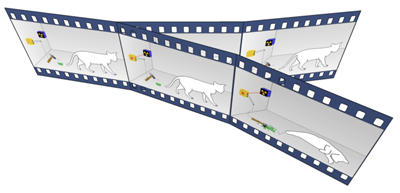
\includegraphics[width=0.6\textwidth]{figs/2022-01-17-13-13-18.png} \\
    \end{center} 
    \begin{quote}
    "Anyone who claims to understand quantum theory is either lying or crazy." \\
    \rightline{$\cdots$ R. P. Feynman \hspace{3em}}   
    \end{quote}
\end{frame}



                        %
%%%%%%%%%%%%%%%%%%%%%%%%%%%%%%%%%%%%55%%
\begin{frame} [plain]
    \frametitle{}
    \Background[1] 
    \begin{center}
    { {\huge 第六讲、力学量算符 }}
    \end{center}  
    \addtocounter{framenumber}{-1}   
\end{frame}
%%%%%%%%%%%%%%%%%%%%%%%%%%%%%%%%%%

%%%%%%%%%%%%%%%%%%%%%%%%%%%%%%%%%
\begin{frame}
        \frametitle{主要内容}
        \transfade
        \tableofcontents
        \addtocounter{framenumber}{-1} 
\end{frame}
%%%%%%%%%%%%%%%%%%%%%%%%%%%%%%%%%%

\section{前情回顾}

\begin{frame}
    \frametitle{前情回顾}
    \begin{itemize}
        \item 波粒二象性
        \item 波函数假说
        \item 波函数的统计解释
        \item 态叠加原理
        \item 薛定谔方程
    \end{itemize}
    ~~\\ \vspace{1.0em}
    \hspace{2em}\alert{TIPS:}这些都是有关量子态的问题,那物理量又如何呢?
\end{frame} 

\section{力学量算符}

\begin{frame} 
    \frametitle{}
    \begin{exampleblock}{考察平均值问题}
        已知粒子的位置波函数$\psi(x,t)$,求动量的期望值   
    \end{exampleblock}
    \alert{解:} 由概率解释知,位置的期望值为
    \begin{equation*}
        \bar{x}=\int x|\psi(x, t)|^{2} d x=\int \psi^{*}(x, t) x \psi(x, t) d x
    \end{equation*}
    对于动量波函数 $c(p,t)$, 动量的期望值为
    \begin{equation*}
        \bar{p_x}=\int p_x|c(p_x, t)|^{2} d p_x=\int c^{*}(p_x, t) p c(p_x, t) d p_x
    \end{equation*}
    很明显,对于已知位置波函数$\psi(x,t)$的条件下,
    \begin{equation*}
        \bar{p_x}\neq\int p_x|\psi(x, t)|^{2} d p_x
    \end{equation*}
\end{frame} 

\begin{frame}
    但可以通过变换求解(注:为了方便,用$p \to p_x$)
    \begin{equation*}
        \begin{split}
            \bar{p}&=\int c^{*}(p) p c(p) d p \\  
            &=\int (\frac{1}{\sqrt{2 \pi \hbar}} \int \psi^{*}(x) e^{\frac{i}{\hbar} p\cdot x} d x) p c\left(p\right) d p \\
            &=\frac{1}{\sqrt{2 \pi \hbar}} \int \int \psi^{*}(x) (e^{\frac{i}{\hbar} p\cdot x}  p) c\left(p\right) d xd p \\
            &=\frac{1}{\sqrt{2 \pi \hbar}} \int \int \psi^{*}(x) (-i\hbar\frac{d}{d x} e^{\frac{i}{\hbar} p\cdot x}) c(p) d xd p \\
            &=\int \psi^{*}(x) (-i\hbar\frac{d}{d x}) (\frac{1}{\sqrt{2 \pi \hbar}} \int e^{\frac{i}{\hbar} p\cdot x} c(p) d p)  d x\\
            &=\int \psi^{*}(x) (-i\hbar\frac{d}{d x}) \psi(x)  d x\\
         \end{split}
    \end{equation*}  
\end{frame} 

\begin{frame}
    定义如下计算符号:
    $$ \hat{p}_x= -i\hbar\frac{d}{d x} $$ 
    上式变为:         
    $$\bar{p}_x=\int \psi^{*}(x) \hat{p}_x \psi(x) d x $$
    称$ \hat{p}_x= -i\hbar\dfrac{d}{d x} $ 是位置表象里的动量算符($x$分量)\\
    同理,任意力学量F的也有算符$\hat{F}$,其平均值为\\
    $$\bar{F}=\int \psi^{*}(x) \hat{F} \psi(x) d x $$
    由此, 我们发现算符与物理量关系密切
\end{frame} 

\begin{frame} 
    \frametitle{一般力学量算符的获取}
    \begin{tcolorbox1}{命题:}
    已知两个基本力学量的算符形式
    \begin{itemize}
        \item  位置算符: $ \hat{\vec{r}} =\vec{r} $
        \item  动量算符: $ \hat{\vec{p}} =-i\hbar(\dfrac{d}{d x}+ \dfrac{d}{d y} + \dfrac{d}{d z})=-i\hbar \nabla $
    \end{itemize}
    求其他一般力学量的算符形式
    \end{tcolorbox1}
    \alert{Bohm规则(1954):} 经典物理学存在力学量F,它若是位置与动量的函数
    \[F(\vec{r},\vec{p})\]
    则其在量子力学中的算符为:
    \[\hat{F}=F(\hat{\vec{r}},\hat{\vec{p}})\]
\end{frame} 

\begin{frame}    
    \begin{exampleblock}{例如:}
        \begin{itemize}
            \item  动能: $ T=\dfrac{p^2}{2\mu} \to \hat{T}= \dfrac{\hat{p}^2}{2\mu} $
            \item  哈密顿量: $ H=T+U(\vec{r} ) \to \hat{H}= \hat{T}+ U(\hat{\vec{r}})$
            \item  角动量:$ \vec{L}=\vec{r}\times\vec{p} \to \hat{\vec{L}}=\hat{\vec{r}}\times \hat{\vec{p}}$
        \end{itemize}
    \end{exampleblock}  
    \alert{TIPS:} 若 $F(\vec{r},\vec{p})$ 中存在连乘项: 
    \[\vec{r}^m\cdot\vec{p}^n\] 
    则采用如下方式进行取代
    \[\frac{1}{2}(\hat{\vec{r}}^m\cdot\hat{\vec{p}}^n+\hat{\vec{p}}^n\cdot\hat{\vec{r}}^m)\]
\end{frame} 

\begin{frame} 
    \alert{例1:} 求经典物理量$F=x^2p_x$的量子力学算符形式 \\ 
    \alert{解:} 根据Bohm规则,有:
    \[\begin{aligned}
        \hat{F}&=\frac{1}{2} (\hat{x}^2 \hat{p}_x + \hat{p}_x \hat{x}^2 ) \\
    \end{aligned}\]   
\end{frame}     

\begin{frame}    
    \begin{tcolorbox4}[Basic assumption 3/5]
    如果物体的状态用波函数描述,则其力学量用算符描述!
    \end{tcolorbox4}
\end{frame} 

\section{算符的类型}

\begin{frame} 
    \frametitle{}
    算符的一般性定义:
    \begin{definition}
        算符:描述态函数之间的对应关系,即算符作用于一个态函数,使它变成另一个态函数。
        $$ \hat{F} \Psi=\psi$$
    \end{definition}
    注:,在不引起不明意义的条件下,为简单见可略去算符的帽子
    \begin{definition}
        单位算符:
        $$ I\Psi=\Psi $$
    \end{definition}
\end{frame} 

\begin{frame}
    \begin{definition}
        算符相等 : 对任意波函数,有
        $$ A\Psi=B\Psi \to A=B $$
    \end{definition}
    \begin{definition}
        算符的和 : 
        $$ (A+B)\Psi=A\Psi+B\Psi $$
        存在交换律和结合律\\
        A+B=B+A\\
        (A+B)+C=A+(B+C)
    \end{definition}
\end{frame} 

\begin{frame}
    \begin{definition}
        算符的积: 
        $$ (AB)\Psi=A(B\Psi) $$
        不存在交换律
        $AB=BA$ 或 $AB\ne BA$ 都有可能
    \end{definition}
    \begin{definition}
        对易子: 
        $$ [A,B]=AB-BA$$
        若[A,B]=0,称两算符对易,否则不对易
    \end{definition}
\end{frame} 

\begin{frame}
    \begin{definition}
        逆算符: 
        $$ F\Psi=\psi $$
        $$ F^{-1}\psi=\Psi $$
    \end{definition}
    \begin{definition}
        内积: 
        $$ \int\Psi^*\psi d \tau$$
        称为两函数的内积,
    \end{definition} 
        内积可以简写成
        $$ (\Psi,\psi)$$ 
        $$ <\Psi|\psi>$$
        并称 $ <\psi|$为左矢, $|\psi>$为右矢\\
    \end{frame} 

    \begin{frame}        
        内积性质:
        $$ (\Psi,\psi)^*=(\psi,\Psi)$$ 
        $$ (\Psi,c_1\psi_1+c_2\psi_2)=(\Psi,c_1\psi_1)+(\Psi,c_2\psi_2)$$ 
        $$ (\Psi,c\psi)=c(\Psi,\psi)$$ 
        $$ (c\Psi,\psi)=c^*(\Psi,\psi)$$ 
  
    \begin{definition}
        伴算符: 
        $$ F|\Psi> = |\psi> $$
        $$ <\psi| = <\Psi|F^{\dagger} $$
        内积形式:
        $$ (\psi,F\Psi)=(\psi,\psi)$$ 
        $$ (F^\dagger \Psi,\psi)=(\psi,\psi)$$ 
    \end{definition}  
\end{frame} 

\begin{frame} 
        \begin{definition}
        线性算符:对任意函数,有\\
        $$F(c_1\psi_1+c_2\psi_2 ) = c_1(F\psi_1)+c_2(F\psi_2 )$$
    \end{definition}
    \begin{definition}
        自伴算符: 
        $$ F^{+} = F $$
        性质:
        $$ (\Psi,F\psi)=(F\Psi,\psi)$$ 
        也称厄密性,即厄密算符就是自伴算符
    \end{definition} 
\end{frame} 

\begin{frame}
    \begin{definition}
        幺正(酉)算符: 
        $$ F^{\dagger}F = FF^{\dagger}=I $$
        性质:
        $$ F^{\dagger}=F^{-1}$$ 
    \end{definition}         
\end{frame} 

\section{力学量算符的性质(一)}

\begin{frame} 
    \frametitle{力学量算符的性质(一)}
    \begin{tcolorbox1}{命题1:}
      可观测力学量算符都是线性算符  
    \end{tcolorbox1}
    \alert{证明:}
        设$\psi_1, \psi_2$ 是算符$\hat{F}$的属于本征值$f$的两个解,有\\
        $$\hat{F}\psi_1=f\psi_1, \to c_1\hat{F}\psi_1=c_1f\psi_1 $$
        $$\hat{F}\psi_2=f\psi_2, \to c_2\hat{F}\psi_2=c_2f\psi_2 $$
        $$f(c_1f\psi_1+c_2f\psi_2)=c_1\hat{F}\psi_1+c_2\hat{F}\psi_2$$
        $$\hat{F}(c_1f\psi_1+c_2f\psi_2)=c_1\hat{F}\psi_1+c_2\hat{F}\psi_2$$
    证毕!
\end{frame} 

\begin{frame} 
    \begin{tcolorbox1}{命题2:}
        可观测力学量算符都是厄密算符  
    \end{tcolorbox1}
    \alert{证明:}
        对任意波函数$\Psi$, 力学量算符$F$的期望值为\\
        $$\bar{F}=(\Psi,\hat{F} \Psi) $$
        $$\bar{F}^*=(\Psi, \hat{F} \Psi)^* = (\hat{F}\Psi, \Psi) $$
        可观测力学量的期望值都是实数,有:\\
        $$(\Psi,\hat{F}\Psi)=(\hat{F} \Psi, \Psi) $$
\end{frame} 

\begin{frame} [allowframebreaks=]
        取 $\Psi= \psi_1+c\psi_2 $, 代入上式,得:
        $$([\psi_1+c\psi_2],\hat{F} [\psi_1+c\psi_2])=(\hat{F}[\psi_1+c\psi_2],[\psi_1+c\psi_2]) $$
        进行积分,得:
        $$
        \begin{array}{r}
        \left(\psi_{1}, \hat{F} \psi_{1}\right)+c^{*}\left(\psi_{2}, \hat{F} \psi_{1}\right)+c\left(\psi_{1}, \hat{F} \psi_{2}\right)+|c|^{2}\left(\psi_{2}, \hat{F} \psi_{2}\right) \\
        =\left(\hat{F} \psi_{1}, \psi_{1}\right)+c^{*}\left(\hat{F} \psi_{2}, \psi_{1}\right)+c\left(\hat{F} \psi_{1}, \psi_{2}\right)+|c|^{2}\left(\hat{F} \psi_{2}, \psi_{2}\right)
        \end{array}
        $$
        算符的平均值都是实数,即 
        $$(\psi_1,\hat{F}\psi_1)=(\hat{F} \psi_1, \psi_1), \qquad (\psi_2,\hat{F}\psi_2)=(\hat{F} \psi_2, \psi_2) $$
        上式可消去第一、四项,变为:
        $$\begin{array}{r}
            c^{*}\left(\psi_{2}, \hat{F} \psi_{1}\right)+c\left(\psi_{1}, \hat{F} \psi_{2}\right) \\
            =c^{*}\left(\hat{F} \psi_{2}, \psi_{1}\right)+c\left(\hat{F} \psi_{1}, \psi_{2}\right)
        \end{array}$$
        分别取$c=1$, $c=i$代入,得到两个等式:
        $$  \left(\psi_{2}, \hat{F} \psi_{1}\right)+\left(\psi_{1}, \hat{F} \psi_{2}\right) = 
        \left(\hat{F} \psi_{2}, \psi_{1}\right)+\left(\hat{F} \psi_{1}, \psi_{2}\right) , \cdots (1)
        $$
        $$
        -i\left(\psi_{2}, \hat{F} \psi_{1}\right)+i\left(\psi_{1}, \hat{F} \psi_{2}\right) 
        =-i\left(\hat{F} \psi_{2}, \psi_{1}\right)+i\left(\hat{F} \psi_{1}, \psi_{2}\right)
        $$
        第二式乘以$i$,得:
        $$
        \left(\psi_{2}, \hat{F} \psi_{1}\right)-\left(\psi_{1}, \hat{F} \psi_{2}\right) 
        =\left(\hat{F} \psi_{2}, \psi_{1}\right)-\left(\hat{F} \psi_{1}, \psi_{2}\right), \cdots (2)
        $$
        (1)+(2),并两边除以2,得
        $$
        \left(\psi_{2}, \hat{F} \psi_{1}\right) =\left(\hat{F} \psi_{2}, \psi_{1}\right)
        $$
        证毕!
\end{frame} 
  
%
%%%%%%%%%%%%%%%%%%%%%%%%%%%%%%%%%%%%%%%%%%%
\begin{frame}
    \frametitle{}
    \begin{center}
    { {\huge 第七讲、厄密算符的性质}}
    \end{center}    
\end{frame}
%%%%%%%%%%%%%%%%%%%%%%%%%%%%%%%%%%%%%


\section{前情回顾}

\begin{frame}
    \frametitle{前情回顾}
    \begin{itemize}
        \item 波函数描述体系的状态
        \item 算符给出体系的物理量
        \item 力学量算符是线性厄密算符
    \end{itemize}
\end{frame} 

\section{厄密算符运算性质}

\begin{frame}
    \frametitle{运算性质}
    \begin{enumerate}
        \item 两厄米算符之和仍为厄米算符
        \item 当且仅当两厄米算符对易时,它们之积才是厄米算符。
        \item 无论两厄米算符是否对易,算符$\dfrac{1}{2}(AB+BA)$ 及$\dfrac{1}{2i}(AB-BA) $  都是厄米算符。
        \item 任意算符总可以分解成$A=A_+ +iA_-$,且$A_+$和$A_-$,都是厄米算符
    \end{enumerate}
\end{frame} 

\begin{frame} [allowframebreaks=]
    \frametitle{}
    \begin{exampleblock}{}
        1、试证明两厄米算符之和仍为厄米算符
    \end{exampleblock}
    \alert{证明:}A,B为厄米算符,则对于任意态,有\\
    $$(\psi, A\psi ) = (A\psi, \psi), \qquad (\psi, B\psi ) = (B\psi, \psi)$$
    对于它们的和,有: \\
    \begin{equation*}
        \begin{split}
            (\psi, (A+B)\psi ) &= (\psi, A\psi ) + (\psi, B\psi ) \\  
            &=(A\psi, \psi ) + (B\psi, \psi ) \\
            &=((A+B)\psi, \psi ) 
         \end{split}
    \end{equation*}  
    证毕!
\end{frame} 

\begin{frame} [allowframebreaks=]
    \frametitle{}
    \begin{exampleblock}{}
        2、当且仅当两厄米算符对易时,它们之积才是厄米算符。
    \end{exampleblock}
    \alert{证明:}A,B为厄米算符,则对于任意态,
    \begin{equation*}
        \begin{split}
            (\psi, (AB)\psi ) &= (\psi, A(B\psi) ) \\  
            &=((A \psi), (B\psi) )  \\
            &=(B(A \psi), \psi )  \\
            &=( (BA) \psi, \psi )  \\
            &=( (AB) \psi, \psi )  \\
         \end{split}
    \end{equation*}  
    证毕!
\end{frame}  

\begin{frame} [allowframebreaks=]
    \frametitle{}
    \begin{exampleblock}{}
        3、无论两厄米算符是否对易,算符$\dfrac{1}{2}(AB+BA)$ 及 $\dfrac{1}{2i}(AB-BA) $ 都是厄米算符
    \end{exampleblock}
    \alert{证明:}A,B为厄米算符,则对于任意态,
    \begin{equation*}
        \begin{split}
            (\psi, \dfrac{1}{2}(AB+BA)\psi ) &=\dfrac{1}{2}(\psi, AB\psi) + \dfrac{1}{2}(\psi, BA\psi)  \\
            &=\dfrac{1}{2}(A\psi, B\psi) + \dfrac{1}{2}(B\psi, A\psi)  \\
            &=\dfrac{1}{2}(BA\psi, \psi) + \dfrac{1}{2}(AB\psi, \psi)  \\
            &=\dfrac{1}{2}((BA+AB)\psi, \psi) \\
            &=(\dfrac{1}{2}(BA+AB)\psi, \psi) \\
            &=(\dfrac{1}{2}(AB+BA)\psi, \psi) 
         \end{split}
    \end{equation*}  
    \begin{equation*}
        \begin{split}
            (\psi, \dfrac{1}{2i}(AB-BA)\psi ) &= (\psi, \dfrac{1}{2i}AB\psi) - (\psi, \dfrac{1}{2i}BA\psi)\\  
            &=\dfrac{1}{2i}(\psi, AB\psi) - \dfrac{1}{2i}(\psi, BA\psi)  \\
            &=\dfrac{1}{2i}(A\psi, B\psi) - \dfrac{1}{2i}(B\psi, A\psi)  \\
            &=\dfrac{1}{2i}(BA\psi, \psi) - \dfrac{1}{2i}(AB\psi, \psi)  \\
            &=-(\dfrac{1}{2i}BA\psi, \psi) +(\dfrac{1}{2i}AB\psi, \psi)  \\
            &=(\dfrac{1}{2i}(AB-BA)\psi, \psi) \\
         \end{split}
    \end{equation*}  
    证毕!
\end{frame}  

\begin{frame} [allowframebreaks=]
    \frametitle{}
    \begin{exampleblock}{}
        4、任意算符总可以分解成$A=A_+ +iA_-$,且$A_+$和$A_-$,都是厄米算符
    \end{exampleblock}
    \alert{证明:}令:
    $$A_+=\dfrac{1}{2} (A+A^+), \qquad A_+=\dfrac{1}{2i} (A-A^+) $$
    有$A=A_+ +iA_-$, 问题转化为证$\dfrac{1}{2} (A+A^+), \qquad \dfrac{1}{2i} (A-A^+) $是厄米算符\\
    \begin{equation*}
        \begin{split}
            (\psi, \dfrac{1}{2} (A+A^+)\psi ) &=\dfrac{1}{2}(\psi, (A)\psi) + \dfrac{1}{2}(\psi, (A^+)\psi) \\
            &= \dfrac{1}{2}((A^+)\psi, \psi) + \dfrac{1}{2}((A^+)^+\psi, \psi) \\
            &= \dfrac{1}{2}((A^+)\psi, \psi) + \dfrac{1}{2}(A\psi, \psi) \\
            &= \dfrac{1}{2}( (A^+ + A) \psi, \psi ) =( \dfrac{1}{2}(A+A^+) \psi, \psi ) 
         \end{split}
    \end{equation*}  
\end{frame} 

\section{厄密算符本征性质}

\begin{frame}
    \frametitle{本征方程}
    厄密算符A的本征方程为
    $$ A\psi=a \psi $$
    称a是算符A的本征值,$\psi$是属于本征值a的本征函数
\end{frame} 

\begin{frame}
    \frametitle{本征性质}
    \begin{enumerate}
        \item 厄米算符的本征值为实数
        \item 任意态下平均值为实数的算符必为厄米算符
        \item 厄米算符属于不同本征值的本征函数正交
        \item 简并的本征函数可通过重组变得正交
        \item 厄米算符的本征函数系具有完备性
        \item 厄米算符的本征函数系具有封闭性
    \end{enumerate}
\end{frame} 
\begin{frame} [allowframebreaks=]
    \frametitle{}
    \begin{exampleblock}{}
        1、试证明厄米算符的本征值为实数
    \end{exampleblock}
    \alert{证明:}设A为厄米算符,有如下本征方程
    $$A\psi=a\psi $$
    \begin{equation*}
        (\psi, A\psi)=(\psi, a\psi)=a(\psi, \psi)
    \end{equation*}  
    由于厄米性,有:
    \begin{equation*}
        (\psi, A\psi)=(A\psi, \psi)=(a\psi, \psi)= a^* (\psi, \psi)
    \end{equation*}
    有:
    \begin{equation*}
        a(\psi, \psi)= a^* (\psi, \psi)
    \end{equation*}
    所以,本征值 a必为实数。
\end{frame} 

\begin{frame} [allowframebreaks=]
    \frametitle{}
    \begin{exampleblock}{}
        2、任意态下平均值为实数的算符必为厄米算符
    \end{exampleblock}
    \alert{证明:}任意态$\Psi$下,F的平均值
    $$(\Psi,F\Psi)=\bar{F}=\bar{F}^*=(\Psi,F\Psi)^*=(F\Psi,\Psi), \qquad (1) $$
    令 $\Psi= \psi_1+c\psi_2 $, 代入上式,得:
    $$([\psi_1+c\psi_2],F [\psi_1+c\psi_2])=(F[\psi_1+c\psi_2],[\psi_1+c\psi_2]) $$
    进行积分,得:
    $$
    \begin{array}{r}
    \left(\psi_{1}, F \psi_{1}\right)+c^{*}\left(\psi_{2}, F \psi_{1}\right)+c\left(\psi_{1}, F \psi_{2}\right)+|c|^{2}\left(\psi_{2}, \hat{F} \psi_{2}\right) \\
    =\left(F \psi_{1}, \psi_{1}\right)+c^{*}\left(F \psi_{2}, \psi_{1}\right)+c\left(F \psi_{1}, \psi_{2}\right)+|c|^{2}\left(\hat{F} \psi_{2}, \psi_{2}\right)
    \end{array}
    $$
    由(1)有: 
    $$(\psi_1,F\psi_1)=(F \psi_1, \psi_1), \qquad (\psi_2,F\psi_2)=(F \psi_2, \psi_2) $$
    上式可消去第一、四项,变为:
    $$\begin{array}{r}
        c^{*}\left(\psi_{2}, F \psi_{1}\right)+c\left(\psi_{1}, F \psi_{2}\right) \\
        =c^{*}\left(F \psi_{2}, \psi_{1}\right)+c\left(F \psi_{1}, \psi_{2}\right)
    \end{array}$$
    分别取$c=1$, $c=i$代入,得到两个等式:
    $$  \left(\psi_{2}, F \psi_{1}\right)+\left(\psi_{1}, F \psi_{2}\right) = 
    \left(\hat{F} \psi_{2}, \psi_{1}\right)+\left(\hat{F} \psi_{1}, \psi_{2}\right) , \cdots (2)
    $$
    $$
    -i\left(\psi_{2}, F \psi_{1}\right)+i\left(\psi_{1}, F \psi_{2}\right) 
    =-i\left(\hat{F} \psi_{2}, \psi_{1}\right)+i\left(F \psi_{1}, \psi_{2}\right)
    $$
    第二式乘以$i$,得:
    $$
    \left(\psi_{2}, F \psi_{1}\right)-\left(\psi_{1}, F \psi_{2}\right) 
    =\left(\hat{F} \psi_{2}, \psi_{1}\right)-\left(F \psi_{1}, \psi_{2}\right), \cdots (3)
    $$
    (2)+(3),并两边除以2,得
    $$
    \left(\psi_{2}, F \psi_{1}\right) =\left(F \psi_{2}, \psi_{1}\right)
    $$
\end{frame} 
\begin{frame} [allowframebreaks=]
    \frametitle{}
    \begin{exampleblock}{}
        3、试证厄米算符属于不同本征值的本征函数正交
    \end{exampleblock}
    \alert{证明:}设$\psi_a$、$\psi_b$分别是厄米算符A属于本征值a、b的本征函数
    \begin{equation*}
        (\psi_a, A\psi_b)=(\psi_a, b\psi_b)=b(\psi_a, \psi_b)
    \end{equation*}  
    由于厄米性,有:
    \begin{equation*}
        (\psi_a, A\psi_b)=(A\psi_a, \psi_b)=a(\psi_a, \psi_b)
    \end{equation*}
    由于$a\neq b$,有
    \begin{equation*}
        (\psi_a, \psi_b)=0
    \end{equation*}
   证毕!
\end{frame} 

\begin{frame} [allowframebreaks=]
    \frametitle{}
    \alert{本征函数的正交归一性}\\
    设$\psi_n$、$\psi_m$都是厄米算符A的本征函数\\
    归一性:
    \begin{equation*}
        (\psi_n, \psi_m)=(\psi_n, \psi_n)=1, \qquad (n=m)
    \end{equation*}  
    正交性:
    \begin{equation*}
        (\psi_n, \psi_m)=1, \qquad (n\neq m)
    \end{equation*}
    定义$\delta$函数:
    \begin{equation*}
        \delta_{n m}= 
        \begin{cases}1, & n=m \\ 
            0, & n \neq m
        \end{cases}
        \end{equation*}
    正交归一性:
    \begin{equation*}
        (\psi_n, \psi_m)=\delta_{nm}
    \end{equation*}
\end{frame} 

\begin{frame} [allowframebreaks=]
    \frametitle{}
    \begin{exampleblock}{}
        4、简并的本征函数可通过重组变得正交
    \end{exampleblock}
    \alert{证明:}设厄米算符A属于本征值a的本征函数有f个
    \begin{equation*}
        A\psi_{na})=a\psi_{na}, \qquad (n=1,2,3,\cdots, f)
    \end{equation*}  
    由这f函数构成如下线性叠加态
    \begin{equation*}
        \Psi_a=\sum_{n=1}^{f} c_n \psi_{na} \qquad (n=1,2,3,\cdots, f)
    \end{equation*}
    这样的叠加态也有f个
    \begin{equation*}
        \Psi_{\beta a}=\sum_{n=1}^{f} c_{\beta n} \psi_{na} \qquad (\beta=1,2,3,\cdots, f)
    \end{equation*}
    \begin{equation*}
        A\Psi_{\beta a}=\sum_{n=1}^{f} c_{\beta n} A\psi_{na} =a \Psi_{\beta a}
    \end{equation*}
   说明叠加态也是属于本征值a的本征函数。\\
   选择系数$c_{\beta n}$,让这f个新的本征态正交归一
   \begin{equation*}
    (\Psi_{\beta a}, \Psi_{\beta' a})=\delta_{\beta\beta'}
    \end{equation*}
    正交条件式数目 $\dfrac{1}{2}f(f-1)$, 归一条件式数目 $f$\\
    系数$c_{\beta n}$的数目为$f^2$,有:$$ f^2\le \dfrac{1}{2}f(f-1)+f$$
    因此,总可以找到一组系数$c_{\beta n}$,使其满足正交归一化条件。
\end{frame} 

\begin{frame} [allowframebreaks=]
    \frametitle{}
    \begin{exampleblock}{}
        试采用Schmidt正交化方案使能量E的三个简并函数($\Psi_1, \Psi_2, \Psi_3$)正交
    \end{exampleblock}
    \alert{解:}取$\psi_1=\dfrac{\Psi_1}{(\Psi_1, \Psi_1)}$\\
    设 $\psi_2'=\Psi_2-(\psi_1, \Psi_2)\psi_1$\\
    \begin{equation*}
        (\psi_1, \psi_2')=(\psi_1, \Psi_2)-(\psi_1, \Psi_2)(\psi_1, \psi_1)=0
    \end{equation*}  
    取$\psi_2=\dfrac{\psi_2'}{(\psi_2', \psi_2')}$\\
    设 $\psi_3'=\Psi_3-(\psi_1, \Psi_3)\psi_1-(\psi_2, \Psi_3)\psi_2$\\
    \begin{equation*}
        (\psi_1, \psi_3')=(\psi_1, \Psi_3)-(\psi_1, \Psi_3)(\psi_1, \psi_1)-(\psi_2, \Psi_3)(\psi_1, \psi_2)=0
    \end{equation*}
    \begin{equation*}
        (\psi_2, \psi_3')=(\psi_2, \Psi_3)-(\psi_1, \Psi_3)(\psi_2, \psi_1)-(\psi_2, \Psi_3)(\psi_2, \psi_2)=0
    \end{equation*}
    取$\psi_3=\dfrac{\psi_3'}{(\psi_3', \psi_3')}$\\
    则$\psi_1, \psi_2, \psi_3$构成正交归一化组。\\
    现在求它们的本征值$\dots$\\
    $$ H\psi_1= H \dfrac{\Psi_1}{(\Psi_1, \Psi_1)} =  \dfrac{E\Psi_1}{(\Psi_1, \Psi_1)} = E \psi_1$$
    $$ H\psi_2= H \dfrac{\Psi_2-(\psi_1, \Psi_2)\psi_1}{(\psi_2', \psi_2')} =  \dfrac{H\Psi_2-(\psi_1, \Psi_2)H\psi_1}{(\psi_2', \psi_2')}=E\psi_2$$
    同理,有$ H\psi_3=E\psi_3$\\
    说明它们依然是简并的!
\end{frame} 

\begin{frame} [allowframebreaks=]
    \frametitle{}
    \begin{exampleblock}{}
        5、厄米算符的本征函数系具有完备性
    \end{exampleblock}
    \alert{完备性定义:}设某个体系的厄米算符A具有本征方程
    \begin{equation*}
        A\psi_{n}=a_n\psi_{n}, 
    \end{equation*}  
    则这个体系的任意态函数都可以在A的本征函数系上展开,
    \begin{equation*}
        \Psi=\sum_n c_n \psi_{n} \qquad (n=1,2,3,\cdots)
    \end{equation*}
    本征函数系的这种性质称为完备性。\\
    (完备性证明?)
    \begin{exampleblock}{}
        试证明展开系数就是态矢量在对应本征基矢上的投影
    \end{exampleblock}
    \begin{equation*}
        c_n=\sum_m c_m\delta_{nm} = \sum_m c_m(\psi_n, \psi_m)= (\psi_n, \sum_m c_m\psi_m) =(\psi_n, \Psi)
    \end{equation*}
    \begin{exampleblock}{}
        试证明展开系数的模方$|c_n|^2$就是测得本征值$a_n$的概率
    \end{exampleblock}
    \begin{equation*}
        \begin{split}
            \bar{A}&=(\Psi, A\Psi)=(\Psi, A\sum_n c_n \psi_{n})\\
            &=(\Psi, \sum_n c_n A\psi_{n})\\
            &=(\sum_m c_m \psi_{m}, \sum_n c_n a_n \psi_{n})\\
            &=\sum_{m,n} c_m^* c_n a_n (\psi_m, \psi_n)\\
            &=\sum_{m,n} c_m^* c_n a_n \delta_{mn}\\
            &=\sum_{n} c_n^* c_n a_n =\sum_{n} |c_n|^2 a_n 
        \end{split}
    \end{equation*}
\end{frame} 

\begin{frame} [allowframebreaks=]
    \frametitle{}
    \begin{exampleblock}{}
        6、厄米算符的本征函数系具有封闭性
    \end{exampleblock}
    \begin{equation*}
        \begin{split}
            \Psi(x)&=\sum_n c_n \psi_{n}(x) \\
            &=\sum_n (\psi_n(x'), \Psi(x')) \psi_{n}(x)\\
            &= (\sum_n\psi_{n} ^* (x)\psi_n(x'), \Psi(x')) \\
            \to &\sum_n\psi_{n} ^* (x)\psi_n(x')=\delta(x-x')\\
            \to &(\psi_{n}(x),\psi_n(x'))=\delta(x-x')
        \end{split} 
    \end{equation*}
\end{frame} 

\section{希尔伯特空间}

\begin{frame} [allowframebreaks=]
    \frametitle{波函数与矩阵}
    \begin{equation*}
        \begin{split}
            \vec{P}&=\sum_i{x_i\vec{e_i}}, \qquad i=1,2,3 \\
            \Psi&=\sum_n (c_n, \psi_n), \qquad n=1,2,\cdots 
        \end{split}  
    \end{equation*}
    数学上,把正交归一的基矢组{$\vec{e_i}, i=1,2,3$}张开的空间叫三维矢量空间, \\
    有 $\vec{P}\Leftrightarrow(x_1,x_2,x_3)$\\
    把正交归一的本征函数系{$\psi_n, n=1,2,\cdots$}张开的空间叫Hilbert空间,\\
    有 $\Psi\Leftrightarrow(c_1,c_2,\cdots)^T$\\
    下面给出较严格的定义$\cdots$
\end{frame} 

\begin{frame} [allowframebreaks=]
    \frametitle{空间的定义}
    \begin{equation*}
        \begin{split}
            \text{1、定义加法} \quad  &\xi=\psi+\varphi\\
            &\psi+\varphi=\varphi+\psi \qquad (\text{交换律})\\
            &(\psi+\varphi)+\xi=\psi+(\varphi+\xi) \qquad (\text{结合律})\\
            &\psi+\text{O}= \psi \qquad (\text{零元})\\
            &\psi+\varphi= \text{O} \qquad (\text{逆元})\\
        \end{split}  
    \end{equation*}
    \begin{equation*}
        \begin{split}
            \text{2、定义数乘} \quad &\varphi=\psi a\\
            &\psi 1= \psi \qquad (\text{1元})\\
            &(\psi a)b=\psi (ab) \qquad (\text{结合律})\\
            &\psi(a+b)= \psi a+ \psi b \qquad (\text{第一分配律})\\
            &(\psi+\varphi) a= \psi a +\varphi a \qquad (\text{第二分配律})\\
        \end{split}  
    \end{equation*}
    \begin{equation*}
        \begin{split}
            \text{3、定义内积} \quad &c=(\psi, \varphi)\\
            &(\psi, \varphi)= (\varphi,\psi)^* \\
            &(\psi, \varphi+\xi)= (\psi, \varphi) + (\psi, \xi)\qquad (\text{分配律})\\
            &(\psi, \varphi a)= (\psi, \varphi )a \\
            &\Rightarrow (\psi a, \varphi )= (\psi, \varphi )a^* \\
            &(\psi,\psi)= c\le 0\\
        \end{split}  
    \end{equation*}
\end{frame} 

\begin{frame}
   \begin{itemize}
       \item 矢量空间:满足加法和数乘两种运算的集合
       \item 内积空间:满足加法、数乘和内积三种运算的集合
       \item 希尔伯特空间:  完全的内积空间\\
       ~~ \\
       *完全性:对给定任意小的实数$\varepsilon$,总有数N存在,当m, n>N时,有\\
       $$ (\psi_m -\psi_n, \psi_m -\psi_n )< \varepsilon $$
   \end{itemize} 
   ~~\\
   量子力学采用希尔伯特空间表述:\\
   1、希尔伯特空间的态矢量描述体系的状态\\
   2、希尔伯特空间的线性厄米算符给出体系的物理量\\
   3、任一厄米算符的本征函数系是希尔伯特空间的一个正交归一完全基。
\end{frame}   
%%%%%%%%%%%%%%%%%%%%%%%%%%%%%%%%%%%%%%%%%%%
\begin{frame}
    \frametitle{}
    \begin{center}
    { {\huge 第八讲、厄密算符本征方程求解}}
    \end{center}    
\end{frame}
%%%%%%%%%%%%%%%%%%%%%%%%%%%%%%%%%%%%%


\section{前情回顾}

\begin{frame}
    \frametitle{前情回顾}
    \begin{itemize}
        \item 希尔伯特空间的态矢量描述体系的状态
        \item 希尔伯特空间的线性厄米算符给出体系的物理量
        \item 任一厄米算符的本征函数系是希尔伯特空间的一个正交归一完全基
    \end{itemize}   
\end{frame} 

\section{动量算符}
\begin{frame} [allowframebreaks=]
    \frametitle{动量}
    算符:  $\hat{\vec p}=-i\hbar \nabla$ \\
    本征方程: $\hat{\vec p}\psi_{\vec p}=\vec p \psi_{\vec p}$ \\
    解本征方程:
    \begin{equation*}
        \begin{split}
            \hat{p}_x\psi_{p_x}&=p_x \psi_{p_x} \\
            -i\hbar\frac{\partial}{\partial x} psi_{\vec p} &= p_x \psi_{p_x}\\
            \frac{1}{\psi_{p_{x}}} \frac{\partial}{\partial x} \psi_{p_{x}}&=\frac{i p_{x}}{\hbar}\\
            \psi_{p_{x}}&=Ae^{\frac{i}{\hbar}p_x x} \\
            \psi_{p_{x}}&=\frac{1}{\sqrt{2\pi\hbar}}e^{\frac{i}{\hbar}p_x x}
        \end{split} 
    \end{equation*}
    本征函数: $$ \psi_{\vec{p}}(\vec{r})=\frac{1}{(2\pi\hbar)^{3/2}}e^{\frac{i}{\hbar}\vec{p}\cdot \vec{x}}   $$
    本征值谱: 连续
        $$ p \in (-\infty, +\infty) $$
    正交归一性:
        $$ (\psi_{\vec{p}'}, \psi_{\vec{p}}) =\delta(\vec{p}'-\vec{p})$$
    完备性:
    $$ \Psi(\vec{r},t)=\iiint\limits_{-\infty}^{+\infty}c(\vec{p},t) \psi_{\vec{p}}(\vec{r}) dp_xdp_ydp_z $$
    封闭性:$$ (\psi_{\vec{p}}(\vec{r}''), \psi_{\vec{p}}(\vec{r}')) =\delta(\vec{r}''-\vec{r}')$$
\end{frame} 

\section{位置算符}
\begin{frame} [allowframebreaks=]
    \frametitle{位置}
    算符:  $\hat{\vec r}=\vec{r}$ \\
    本征方程: $\hat{\vec r}\psi_{\vec \lambda}=\vec \lambda \psi_{\vec \lambda}$ \\
    解本征方程:
    \begin{equation*}
        \begin{split}
            \hat{\vec r}\psi_{\vec \lambda}&=\vec \lambda \psi_{\vec \lambda} \\
            \vec{r}\psi_{\vec \lambda}&=\vec \lambda \psi_{\vec \lambda} \\
        \end{split} 
    \end{equation*}
    分析,$\vec \lambda$是本征值(常数),所以除 $\vec r =\vec \lambda $这一点外,$\psi_{\vec \lambda}$其他位置
    处处为零,有:
    本征函数: $$ \psi_{\vec \lambda}(\vec{r})= A \delta(\vec{r}-\vec{\lambda})= \delta(\vec{r}-\vec{\lambda})$$
    本征值谱: 连续
        $$ \lambda \in (-\infty, +\infty) $$
    正交归一性:
        $$ (\psi_{\vec{\lambda}'}, \psi_{\vec{\lambda}}) =\delta(\vec{\lambda}'-\vec{\lambda})$$
    完备性:
    $$ \Psi(\vec{r},t)=\iiint\limits_{-\infty}^{+\infty}c_(\vec{\lambda}(\vec{r},t) \psi_{\vec{\lambda}}(\vec{r}') dx'dy'dz' $$
    封闭性:$$ (\psi_{\vec{\lambda}}(\vec{r}''), \psi_{\vec{\lambda}}(\vec{r}')) =\delta(\vec{r}''-\vec{r}')$$
\end{frame} 
\begin{frame} [allowframebreaks=]
    \frametitle{课堂作业}
    \begin{exampleblock}{}
     已知某算符为  $\hat{F}=-ie^{ix}\frac{d}{dx}$,求本征函数 \\   
    \end{exampleblock}
\end{frame} 

\begin{frame} [allowframebreaks=]
    \frametitle{}
    \begin{exampleblock}{}
     已知某算符为  $\hat{F}=-ie^{ix}\frac{d}{dx}$,求本征函数 \\   
    \end{exampleblock}
    \alert{解:} 本征方程为 $\hat{F}\psi_f(x)=f\psi_f(x)$\\
    代入算符的具体形式:
    \begin{equation*}
        \begin{split}
            -ie^{ix}\frac{d}{dx}\psi_f(x)&=f\psi_f(x) \\
            \frac{d\psi_f(x)}{\psi_f(x)}&=ife^{-ix} dx \\
            \frac{d\psi_f(x)}{\psi_f(x)}&=d(-fe^{-ix}) \\
           \ln{\psi_f(x)}&=-fe^{-ix}+\ln c \\
           \psi_f(x)&=c e^{-fe^{-ix}}
        \end{split} 
    \end{equation*}
\end{frame} 

\section{角动量算符}
\begin{frame} [allowframebreaks=]
    \frametitle{角动量算符}
    \begin{exampleblock}{}
     已知角动量的经典定义为:
    $$\vec{L}=\vec{r}\times\vec{p}$$ 
    求其算符形式,并求本征方程   
    \end{exampleblock}
    \alert{解:} 根据对应原则,有:
    $$\hat{\vec{L}}=\hat{\vec{r}}\times\hat{\vec{p}}= -i\hbar \vec{r}\times\nabla$$
    (I)在直角坐标系中,\\
    $$
    \left \{
    \begin{array}{l} 
        \hat{L}_x=y\hat{p}_z-z\hat{p}_y  \\ 
        \hat{L}_y=z\hat{p}_x-x\hat{p}_z  \\ 
        \hat{L}_z=x\hat{p}_y-y\hat{p}_x 
    \end{array}
    \right.
    $$
    $$ \hat{L}^2= \hat{L}_x ^2+ \hat{L}_y ^2 +\hat{L}_z ^2  $$

    (II)在球坐标系中,\\
    $$
    \left\{\begin{array}{l}
        \hat{L}_{x}=i \hbar\left[\sin \varphi \frac{\partial}{\partial \theta}+\cot \theta \cos \varphi \frac{\partial}{\partial \varphi}\right] \\
        \hat{L}_{y}=-i \hbar\left[\cos \varphi \frac{\partial}{\partial \theta}+\cot \theta \sin \varphi \frac{\partial}{\partial \varphi}\right] \\
        \hat{L}_{z}=-i \hbar \frac{\partial}{\partial \varphi}
        \end{array}\right.
    $$
    $$ \hat{L}^{2}=-\hbar^{2}\left[\frac{1}{\sin \theta} \frac{\partial}{\partial \theta}\left(\sin \theta \frac{\partial}{\partial \theta}\right)+\frac{1}{\sin ^{2} \theta} \frac{\partial^{2}}{\partial \varphi^{2}}\right] $$
    相对比较简单,可求解本征方程
\end{frame} 

\begin{frame} [allowframebreaks=]
    \frametitle{解角动量本征方程}
    $\hat{L}_z$ 的本征方程为 $$\hat{L}_z\Phi(\varphi)=l_z\Phi(\varphi)$$
    代入算符的具体形式:
    \begin{equation*}
        \begin{split}
            -i \hbar \frac{\partial}{\partial \varphi}\Phi(\varphi)&=l_z\Phi(\varphi) \\
            \frac{1}{\Phi(\varphi)}\frac{\partial}{\partial \varphi}\Phi(\varphi)&=\frac{i}{\hbar}l_z \\
            \Phi(\varphi)&=A e ^{\frac{i}{\hbar}l_z\varphi}
        \end{split} 
    \end{equation*}
     根据周期性边界条件:$\Phi(\varphi)=\Phi(2\pi+\varphi)$\\
    \begin{equation*}
        \frac{A e ^{\frac{i}{\hbar}l_z(2\pi+\varphi)}}{A e ^{\frac{i}{\hbar}l_z\varphi}}=1
    \end{equation*} 
    \begin{equation*}
        e ^{\frac{i}{\hbar}l_z2\pi}=1
    \end{equation*} 
    $$
    \cos \left(2 \pi l_{z} / \hbar\right)+i \sin \left(2 \pi l_{z} / \hbar\right)=1
    $$
    $$ 2 \pi l_{z} / \hbar=2\pi m, \qquad (m=0,\pm 1,  \pm 2, \cdots) $$
    $$\to l_z=m\hbar$$
    $$\to \Phi_m(\varphi)=Ae^{im\varphi}$$
    归一化:
    \begin{equation*}
        \begin{split}
            \int_0 ^{2\pi} |\Phi|^2 d \varphi &= \int_0 ^{2\pi} \Phi^*\Phi  d \varphi \\
            &= A^2 \int_0 ^{2\pi} e^{im\varphi-im\varphi} d \varphi \\
            &= A^2 2\pi \\
            &= 1
        \end{split}   
    \end{equation*}
    $$ \to A= \frac{1}{\sqrt{2\pi}} $$
    $$ \to \Phi_m(\varphi)=\frac{1}{\sqrt{2\pi}}e^{im\varphi}$$
    (小结)算符:  $\hat{L}_{z}=-i \hbar \frac{\partial}{\partial \varphi}$ \\
    本征方程: $$\hat{L}_z\Phi_m(\varphi)=m\hbar \Phi_m (\varphi)$$
    本征函数: $$ \Phi_m(\varphi)=\frac{1}{\sqrt{2\pi}}e^{im\varphi}$$
    本征值谱:  分立
        $$ l_z=m\hbar, \qquad (m=0,\pm 1,  \pm 2, \cdots) $$
    正交归一性:
        $$ (\Phi_{m'}(\varphi), \Phi_m(\varphi)) =\delta_{m'm}$$
    完备性与封闭性:$$ (\Phi_m(\varphi''), \Phi_m(\varphi')) =\delta(\varphi''-\varphi')$$
\end{frame} 

\begin{frame} [allowframebreaks=]
    \frametitle{}
    $\hat{L}^2$ 的本征方程为 $$\hat{L}^2Y(\theta,\varphi)=l^2 Y(\theta,\varphi)$$
    代入算符的具体形式,并令本征值为$\lambda\hbar^2$,有:
    \begin{equation*}
        \begin{split}
            -\hbar^{2}\left[\frac{1}{\sin \theta} \frac{\partial}{\partial \theta}\left(\sin \theta \frac{\partial}{\partial \theta}\right)+\frac{1}{\sin ^{2} \theta} \frac{\partial^{2}}{\partial \varphi^{2}}\right] Y(\theta,\varphi)&=\lambda\hbar^2 Y(\theta,\varphi) \\
            \left[\frac{1}{\sin \theta} \frac{\partial}{\partial \theta}\left(\sin \theta \frac{\partial}{\partial \theta}\right)+\frac{1}{\sin ^{2} \theta} \frac{\partial^{2}}{\partial \varphi^{2}}\right] Y(\theta,\varphi)&=-\lambda Y(\theta,\varphi) \\
        \end{split} 
    \end{equation*}
    这是球谐方程,利用分离变量及幂级数法可解:\\
    本征值: $$\lambda=l(l+1), \qquad (l= 0,1,2,\cdots)$$
    $\hat{L}^2$的本征值:$$l^2=\lambda\hbar^2=l(l+1)\hbar^2$$
    本征函数:
    $$
    \mathrm{Y}_{l m}(\theta, \varphi)=(-1)^{m} \sqrt{\frac{(2 l+1)(l-m) !}{4 \pi(l+m) !}} \mathrm{P}_{l}^{m}(\cos \theta) \Phi_{m}(\varphi)
    $$ 
    式中:
    $$ m=0,\pm 1,  \pm 2, \cdots, \pm l)  $$
    $\mathrm{P}_{l}^{m} $ 是勒上德多项式
    $$
    P_{l}^{m}(\cos \theta)=(-1)^{l+m} \frac{1}{2^{l} l !} \sqrt{\frac{(2 l+1)}{4 \pi} \frac{(l+m) !}{(l-m) !} \frac{1}{\sin ^{m} \theta}\left(\frac{d}{d \cos \theta}\right)^{l-m} \sin ^{2 l} \theta}
    $$
    (小结)算符:  $$ \hat{L}^{2}=-\hbar^{2}\left[\frac{1}{\sin \theta} \frac{\partial}{\partial \theta}\left(\sin \theta \frac{\partial}{\partial \theta}\right)+\frac{1}{\sin ^{2} \theta} \frac{\partial^{2}}{\partial \varphi^{2}}\right] $$
    本征方程: $$\hat{L}^2Y(\theta,\varphi)=l(l+1)\hbar^2 Y(\theta,\varphi)$$
    本征函数:     $$
    \mathrm{Y}_{l m}(\theta, \varphi)=(-1)^{m} \sqrt{\frac{(2 l+1)(l-m) !}{4 \pi(l+m) !}} \mathrm{P}_{l}^{m}(\cos \theta) \Phi_{m}(\varphi)
    $$ 
    本征值谱:  分立
    $$l^2=l(l+1)\hbar^2, \qquad (l= 0,1,2,\cdots, n) $$
    正交归一性:
    $$
    \int_{0}^{\pi} \int_{0}^{2 \pi} Y_{l m}(\theta, \varphi) Y_{l^{\prime} m^{\prime}}^{*}(\theta, \varphi) \sin \theta \mathrm{d} \theta \mathrm{d} \varphi=\delta_{l l^{\prime}} \delta_{m m^{\prime}}
    $$
    完备性与封闭性:
    $$\psi(\theta, \varphi)=\sum_{l=0}^{n} \sum_{m=-l}^{l} C_{l m} \mathrm{Y}_{l m}(\theta, \varphi)$$

    简并度: $2l+1$\\
    对于本征值$l(l+1)\hbar^2$,有$2l+1$个本征函数 $\mathrm{Y}_{l m}$与之对应。
\end{frame} 

\begin{frame} 
    \frametitle{角动量量子化}
    \begin{wrapfigure} {b} {0.4\textwidth} %;图在右
        \includegraphics[width=0.35\textwidth]{figs/LandL2.png}   
    \end{wrapfigure}
    角动量大小:$\sqrt{l(l+1)\hbar}, \qquad (l=1,2,\cdots, n)$,对应球的半径。\\
    角动量在Z轴上的投影大小 $l_z=m\hbar, \qquad (m=0,\pm 1,\pm 2, \cdots, \pm l)$
\end{frame} 

\section{能量算符}

\begin{frame} 
    \frametitle{}
    \begin{exampleblock}{例1:自由粒子能量本征值}
    求质量为$\mu$的一维自由粒子的能量本征值和本征态  
    \end{exampleblock}
    \alert{解:} 能量算子即哈密顿算子:
    $$ \hat{H}=\hat{T}+\hat{V}=\frac{\hat{p}_x ^2 }{2\mu} = -\frac{\hbar^2}{2\mu}\frac{d^2}{dx^2} $$
    建立能量本征方程:
    $$ \hat{H} \psi =E \psi $$
    $$ -\frac{\hbar^2}{2\mu}\frac{d^2}{dx^2} \psi =E \psi $$
    $$ \frac{d^2}{dx^2} \psi = -\frac{2\mu E}{\hbar^2} \psi $$
\end{frame}

\begin{frame} 
    $$  \psi'' + k^2 \psi =0 $$
    特征方程的根为:$\lambda_{1,2}=\pm k$ \\
    方程的解(本征函数)为: $\psi \sim e^{\pm ikx}$  \\
    能量本征值:$ E= \frac{\hbar^2 k^2 }{2\mu} \le 0 $
\end{frame}


\begin{frame} 
    \frametitle{ }
    \begin{exampleblock}{例2:转子的能量本征值}
    求转动惯量为I的平面转子的能量本征值和本征态  
    \end{exampleblock}
    \alert{解:} 能量算子即哈密顿算子:
    $$ \hat{H}=\hat{T}+\hat{V}=\frac{\hat{l}_z ^2 }{2I} = -\frac{\hbar^2}{2I}\frac{\partial^2}{\partial\varphi^2} $$
    建立能量本征方程:
    $$ \hat{H} \psi =E \psi $$
    $$ -\frac{\hbar^2}{2I}\frac{\partial^2}{\partial\varphi^2} \psi =E \psi $$
\end{frame}

\begin{frame} 
    能量本征函数: $$\psi_m(\varphi)=\frac{1}{\sqrt{2\pi}}e^{im\varphi}, \qquad (m=0,\pm 1, \pm 2, \cdots)$$
    能量本征值: $$ E_m=\frac{m^2\hbar^2}{2I} $$ 
    \begin{exampleblock}{}
     讨论:如何求空间转子的能量本征值和本征态?    
    \end{exampleblock}    
\end{frame}  %                     %
%%%%%%%%%%%%%%%%%%%%%%%%%%%%%%%%%%%%%%%%%%%
\begin{frame}
    \frametitle{}
    \begin{center}
    { {\huge 第九讲、对易关系求解}}
    \end{center}    
\end{frame}
%%%%%%%%%%%%%%%%%%%%%%%%%%%%%%%%%%%%%


\section{前情回顾}

\begin{frame}
    \frametitle{前情回顾}
    \begin{itemize}
        \item 希尔伯特空间的态矢量描述体系状态
        \item 希尔伯特空间的算符给出体系的物理量
        \item 算符的本征函数系构成正交归一完全基
        \item 常见算符本征方程求解
    \end{itemize}   
\end{frame} 

\section{对易子及运算法则}
\begin{frame} 
    \frametitle{}
    \begin{tcolorbox2}{对易子定义:}
        定义对易子:$$ [F,G]\equiv FG-GF $$ \\
        若$[F,G]=0$,则对易 \\
        若$[F,G]\neq0$,则不对易  
    \end{tcolorbox2}
\end{frame} 

\begin{frame} 
    \frametitle{运算法则}
    \begin{enumerate}
        \item  $[A,B]=-[B,A]$
        \item  $[A,A]=0$
        \item  $[A,c]=0$
        \item  $[A,B+C]=[A,B]+[A,C]$
        \item  $[A,BC]=B[A,C]+[A,B]C$
        \item  $[AB,C]=A[B,C]+[A,C]B$
    \end{enumerate}
\end{frame} 
\begin{frame}
    \begin{proof}{}   
        \begin{equation*}
            \begin{split} 
            [AB,C]&=ABC-CAB \\
            A[B,C]+[A,C]B&=A(BC-CB)+(AC-CA)B\\
            &=ABC-ACB+ACB-CAB\\
            &=ABC-CAB
            \end{split}  
        \end{equation*}  
        $$ [AB,C]=A[B,C]+[A,C]B $$
    \end{proof}
\end{frame} 

\begin{frame} 
    \begin{tcolorbox2}{推论:}
        \begin{itemize}
            \item 如果A与B、C对易,则A与$B+C$对易
            \item 如果A与B、C对易,则A与$B^n+C^m$对易
            \item 如果A与B、C对易,则A与$BC$对易
            \item 如果A与B、C对易,则A与$B^nC^m$对易
            \item 如果A与B、C对易,则A与$B^nC^m+B^{n'}C^{m'}$对易
        \end{itemize}
    \end{tcolorbox2}
\end{frame} 

\begin{frame} [allowframebreaks=]
    \begin{proof}{}
        \begin{equation*}
            \begin{split} 
             [A,B^{n}]&=[A,BB^{n-1}] \\
             &=B[A,B^{n-1}]+[A,B]B^{n-1}\\
             &=B[A,B^{n-1}] \\
             &=B^2[A,B^{n-2}]\\
             &=\cdots\\
             &=B^{n-1}[A,B]\\
             &= 0\\
            \end{split}  
        \end{equation*}  
    \end{proof}
    \begin{proof}{}
        同理:$[A,C^{m}]=0$\\
        \begin{equation*}
            \begin{split} 
            [A,B^{n}+C^{m}] &= [A,B^{n}]+[A,C^{m}]\\
            &=0 \\
            [A,B^{n}C^{m}] &= B^{n}[A,C^{m}] + [A,B^{n}] C^{m}\\
            &=0 \\
        \end{split}  
        \end{equation*}
        同理:$[A,B^{n'}C^{m'}]=0$\\
        \begin{equation*}
            \begin{split} 
            [A,B^{n}C^{m}+B^{n'}C^{m'}] &= [A,B^{n}C^{m}]+[A,B^{n'}C^{m'}]\\
            &=0\\
        \end{split}  
        \end{equation*}
    \end{proof}
\end{frame} 

\section{对易关系}
\begin{frame} [allowframebreaks=]
    \begin{tcolorbox1}{1.位置-动量对易关系}
        求位置动量对易关系 $[x,p_x]=?$,  $[x,p_y]=?$
    \end{tcolorbox1}
    \alert{解:} 对任意波函数$\psi$,有
    \begin{equation*}
        \begin{split}
        xp_x\psi&= x(-i\hbar \frac{\partial}{\partial x})\psi \\
        &=-i\hbar x \frac{\partial}{\partial x}\psi\\
        p_x x \psi&= -i\hbar \frac{\partial}{\partial x} (x\psi) \\
        &=-i\hbar\psi - i\hbar x \frac{\partial}{\partial x}\psi \\
        \end{split}  
    \end{equation*}
    两式相减,$$(xp_x-p_x x)\psi= i\hbar\psi$$
    得 $xp_x-p_x x= i\hbar$ \\
    即 $[x,p_x]= i\hbar$\\
    同理,有:\\
    $\begin{cases}
        [x,p_x]= i\hbar  \\ 
        [y,p_y]= i\hbar  \\ 
        [z,p_z]= i\hbar  
    \end{cases}$
    $\begin{cases}
        [x,p_y]= 0  \\ 
        [y,p_z]= 0  \\ 
        [z,p_x]= 0  
    \end{cases}$
    $\begin{cases}
        [p_x,p_y]= 0  \\ 
        [p_y,p_z]= 0  \\ 
        [p_z,p_x]= 0  
    \end{cases}$
    $\begin{cases}
        [x,y]= 0  \\ 
        [y,z]= 0  \\ 
        [z,x]= 0  
    \end{cases}$ \\
    \begin{tcolorbox}[colback=yellow!5,colframe=red!75!black,title=量子力学基本对易关系]
    $\begin{cases}
        [x_\alpha,x_\beta]= 0  \\ 
        [p_\alpha,p_\beta]= 0  \\ 
        [x_\alpha,p_\beta]= i\hbar \delta_{\alpha\beta}  \\ 
    \end{cases}$
    \end{tcolorbox}
\end{frame} 

\begin{frame} [allowframebreaks=]
    \frametitle{}
    \begin{tcolorbox1}{2.角动量-位置对易关系}
        试证明角动量-位置对易关系 $[L_x,y]=i\hbar z,  [L_x,x]=0$
    \end{tcolorbox1}
    \alert{证明:} 
    \begin{equation*}
        \begin{split}
        [L_x,y]&= [yp_z-zp_y,y]\\
        &=-[y,yp_z-zp_y]\\
        &= -[y,yp_z] + [y,zp_y]\\
        &=-y[y,p_z] -[y,y]p_z + z[y,p_y] + [y,z]p_y\\
        &=-0 -0 + z i\hbar + 0\\
        &=i\hbar z \\
        \end{split}  
    \end{equation*}
    同理,有:\\
    $\begin{cases}
        [L_x,y]= i\hbar z  \\ 
        [L_x,x]= 0  \\ 
        [L_x,z]= -i\hbar y 
    \end{cases}$
    $\begin{cases}
        [L_y,z]= i\hbar x  \\ 
        [L_y,y]= 0  \\ 
        [L_y,x]= -i\hbar z 
    \end{cases}$
    $\begin{cases}
        [L_z,x]= i\hbar y  \\ 
        [L_z,z]= 0  \\ 
        [L_z,y]= -i\hbar x 
    \end{cases}$
    \begin{tcolorbox}[colback=yellow!5,colframe=red!75!black,title=角动量-位置对易关系]
        $$ [L_\alpha,x_\beta]= \varepsilon_{\alpha\beta\gamma} i\hbar x_\gamma $$ 
    \end{tcolorbox}
\end{frame} 

\begin{frame} [allowframebreaks=]
    \frametitle{}
    \begin{tcolorbox1}{3.角动量-动量对易关系}
        试证明角动量-动量对易关系 $[L_x,p_y]=i\hbar p_z,  [L_x,p_x]=0$
    \end{tcolorbox1}
    \alert{证明:} 
    \begin{equation*}
        \begin{split}
        [L_x,p_y]&= [yp_z-zp_y,p_y]\\
        &=-[p_y,yp_z-zp_y]\\
        &=-[p_y,yp_z] + [p_y,zp_y]\\
        &=-y[p_y,p_z] -[p_y,y]p_z + z[p_y,p_y] + [p_y,z]p_y\\
        &=-y[p_y,p_z] +[y,p_y]p_z + z[p_y,p_y] + [p_y,z]p_y\\
        &=-0 + i\hbar p_z + 0+0\\
        &=i\hbar p_z \\
        \end{split}  
    \end{equation*}
    同理,有:\\
    $\begin{cases}
        [L_x,p_y]= i\hbar p_z  \\ 
        [L_x,p_x]= 0  \\ 
        [L_x,p_z]= -i\hbar p_y 
    \end{cases}$
    $\begin{cases}
        [L_y,p_z]= i\hbar p_x  \\ 
        [L_y,p_y]= 0  \\ 
        [L_y,p_x]= -i\hbar p_z 
    \end{cases}$
    $\begin{cases}
        [L_z,p_x]= i\hbar p_y  \\ 
        [L_z,p_z]= 0  \\ 
        [L_z,p_y]= -i\hbar p_x 
    \end{cases}$
    \begin{tcolorbox}[colback=yellow!5,colframe=red!75!black,title=角动量-动量对易关系]
        $$ [L_\alpha,p_\beta]= \varepsilon_{\alpha\beta\gamma} i\hbar p_\gamma $$ 
    \end{tcolorbox}
\end{frame} 

\begin{frame} [allowframebreaks=]
    \frametitle{}
    \begin{tcolorbox1}{4.角动量-角动量对易关系}
        试证明位置角动量对易关系 $[L_x,L_y]=i\hbar L_z,  [L_z, L^2]= 0$
    \end{tcolorbox1}
    \alert{证明1:} 基于运算法则
    \begin{equation*}
        \begin{split}
        [L_x,L_y]= &[yp_z-zp_y,zp_x-xp_z]\\
        =&[yp_z,zp_x-xp_z] - [zp_y,zp_x-xp_z]\\
        =&y[p_z,zp_x-xp_z]+[y,zp_x-xp_z]p_z- z[p_y,zp_x-xp_z]-[z,zp_x-xp_z]p_y\\
        =&y[p_z,zp_x]-y[p_z,xp_z]+[y,zp_x]p_z-[y,xp_z]p_z \\ &-z[p_y,zp_x] +z[p_y,xp_z]- [z,zp_x]p_y+[z,xp_z]p_y\\
        =&yz[p_z,p_x]+y[p_z,z]p_x-yx[p_z,p_z]-y[p_z,x]p_z \\ & +z[y,p_x]p_z+[y,z]p_xp_z-x[y,p_z]p_z -[y,x]p_zp_z \\ & -zz[p_y,p_x] -z[p_y,z]p_x +zx[p_y,p_z] +z[p_y,x]p_z \\ & -z[z,p_x]p_y -[z,z]p_xp_y+x[z,p_z]p_y +[z,x]p_zp_y\\  
    \end{split}  
    \end{equation*}
    \begin{equation*}
        \begin{split}
        [L_x,L_y]=&0-yi\hbar p_x-0-0+0+0-0 -0-0 -0 +0 +0-0 -0+xi\hbar p_y +0\\
        =&i\hbar xp_y-i\hbar y p_x\\
        =&i\hbar (xp_y-y p_x)\\
        =&i\hbar L_z\\    
    \end{split}  
    \end{equation*}
    \alert{证明2:} 基于推论 
    \begin{equation*}
        \begin{split}
        [L_x,L_y]= &[yp_z-zp_y,zp_x-xp_z]\\
        =&[yp_z,zp_x-xp_z] - [zp_y,zp_x-xp_z]\\
        =&y[p_z,zp_x-xp_z]+[y,zp_x-xp_z]p_z- z[p_y,zp_x-xp_z]-[z,zp_x-xp_z]p_y\\
        =&y[p_z,zp_x]+0- 0-[z,-xp_z]p_y\\
        =&yz[p_z,p_x]+y[p_z,z]p_x+x[z,p_z]p_y+[z,x]p_zp_y\\
        =&0-yi\hbar p_x+x i\hbar p_y+0\\
        =&i\hbar L_z\\
    \end{split}  
    \end{equation*}
    同理,有:\\
    $\begin{cases}
        [L_x,L_y]= i\hbar L_z  \\ 
        [L_x,L_x]= 0  \\ 
        [L_x,L_z]= -i\hbar L_y 
    \end{cases}$
    $\begin{cases}
        [L_y,L_z]= i\hbar L_x  \\ 
        [L_y,L_y]= 0  \\ 
        [L_y,L_x]= -i\hbar L_z 
    \end{cases}$
    $\begin{cases}
        [L_z,L_x]= i\hbar L_y  \\ 
        [L_z,L_z]= 0  \\ 
        [L_z,L_y]= -i\hbar L_x 
    \end{cases}$
    \begin{tcolorbox}[colback=yellow!5,colframe=red!75!black,title=角动量对易关系]
        $$ [L_\alpha,L_\beta]= \varepsilon_{\alpha\beta\gamma} i\hbar L_\gamma $$ 
    \end{tcolorbox}
\end{frame} 

\begin{frame} [allowframebreaks=]
    \frametitle{}
    \begin{tcolorbox1}{5.角动量对易关系2}
        试证明角动量对易关系 $[L_z,L^2]=0$
    \end{tcolorbox1}
    \alert{证明:} 
    \begin{equation*}
        \begin{split}
        [L_z,L^2]&= [L_z,L_x ^2+L_y ^2+L_z ^2]\\
        &=[L_z,L_x ^2]+[L_z,L_y ^2]+[L_z,L_z ^2]\\
        &=[L_z,L_x ^2]+[L_z,L_y ^2]\\
        &=L_x[L_z,L_x] +[L_z,L_x]L_x +L_y[L_z,L_y] +[L_z,L_y]L_y\\
        &=i\hbar L_x L_y +i\hbar L_yL_x - i\hbar L_x L_y -i\hbar L_yL_x\\
        &=0 \\
        \end{split}  
    \end{equation*}
    同理,有:\\
    $\begin{cases}
        [L_x,L^2]= 0  \\ 
        [L_y,L^2]= 0  \\ 
        [L_z,L^2]= 0 
    \end{cases}$
    \begin{tcolorbox}[colback=yellow!5,colframe=red!75!black,title=角动量对易关系]
        $$ [L_\alpha,L^2]= 0 $$ 
    \end{tcolorbox}
\end{frame} 

\begin{frame} [allowframebreaks=]
    \frametitle{}
    \begin{tcolorbox}[colback=yellow!5,colframe=yellow!75!black,title=课堂作业]
        定义升降算符:$L_\pm \equiv L_x \pm i L_y$ \\
     试证明如下对易关系  $$[L_\pm,L^2]=0$$
     $$[L_z, L_\pm]= \pm \hbar L_\pm $$
    \end{tcolorbox}
\end{frame} 
  %   
%%%%%%%%%%%%%%%%%%%%%%%%%%%%%%%%%%%%%%%%%%%
\begin{frame}
    \frametitle{}
    \begin{center}
    { {\huge 第十讲、对易关系物理含义}}
    \end{center}    
\end{frame}
%%%%%%%%%%%%%%%%%%%%%%%%%%%%%%%%%%%%%


\section{前情回顾}

\begin{frame}
    \frametitle{前情回顾}
    \begin{itemize}
        \item 希尔伯特空间的态矢量描述体系状态
        \item 希尔伯特空间的算符给出体系的物理量
        \item 算符的本征函数系构成正交归一完全基
        \item 常见算符本征方程求解
        \item 算符对易关系求解
    \end{itemize}   
\end{frame} 

\section{对易的含义}
\begin{frame} 
    \frametitle{对易的含义}
    \begin{enumerate}
        \item  相互对易的两力学量算符,具有共同本征函数系
        \item  当体系处于共同的本征态时,它们同时具有确定值
        \item  构成最小完全集的一组力学量算符的数目等于体系的自由度。
    \end{enumerate}
\end{frame} 

\begin{frame} [allowframebreaks=]
    \begin{tcolorbox}[colback=yellow!5,colframe=yellow!75!black,title=定理1:]
        如果两算符具有共同的本征函数系,则它们对易
    \end{tcolorbox}
    \alert{证明:} 设它们的共同本本征函数系为{$\varphi_n$}, 有:\\ 
        \begin{equation*}
            \begin{split} 
            A\varphi_n&=a_n \varphi_n \\
            B\varphi_n&=b_n \varphi_n \\
            \end{split}  
        \end{equation*}  
        对任意波函数
        \begin{equation*}
            \begin{split} 
            [A,B]\Psi &= [A,B]\sum_n c_n \varphi_n \\
            &= \sum_n c_n [A,B]\varphi_n \\
            &= \sum_n c_n (AB-BA)\varphi_n\\
            &= \sum_n c_n AB\varphi_n- \sum_n c_n BA\varphi_n\\
            &= \sum_n c_n a_nb_n\varphi_n- \sum_n c_n a_nb_n\varphi_n\\
            &=0\Psi
            \end{split}  
        \end{equation*}  
        得证: $$[A,B]=0$$
\end{frame} 

\begin{frame} [allowframebreaks=]
    \begin{tcolorbox}[colback=yellow!5,colframe=yellow!75!black,title=逆定理:]
        如果两算符对易,则它们具有共同的本征函数系。
    \end{tcolorbox}
    \alert{证明:} 设A有本征函数系{$\varphi_n$}, 有:\\ 
        \begin{equation*}
            \begin{split} 
            A(B\varphi_n)&= AB\varphi_n\\
            &=BA\varphi_n \\
            &=Ba_n\varphi_n \\
            &=a_n(B\varphi_n) \\
            \end{split}  
        \end{equation*}  
        说明$B\varphi_n$ 和 $\varphi_n$ 都是A的属于本征值$a_n$的本征态,当$a_n$非简并时, 
        $B\varphi_n$ 和 $\varphi_n$ 描述同一个态,两者最多只差一个常数因子,记为 $b_n$,
        $$ B\varphi_n=b_n \varphi_n$$
        即: $\varphi_n$也是B的本征态。\\
        证毕!
\end{frame} 

\begin{frame} [allowframebreaks=]
    \begin{tcolorbox}[colback=yellow!5,colframe=yellow!75!black,title=推论1:]
        一组力学量算符具有共同本征函数完备系的充要条件是这些算符彼此两两对易
    \end{tcolorbox}
    \alert{例子1:动量本征函数系} \\
    由于 $[p_\alpha,p_\beta]=0$,动量算符($p_x, p_y, p_z$)具有共同本征函数系 即平面波\\
    $$ \Psi_{\vec p}= \frac{1}{(2\pi\hbar)^{3/2}} e^{\frac{i}{\hbar}\vec{p}\cdot\vec{r}}$$ 
    \alert{例子2:角动量本征函数系} \\
    由于 $[L_z,L^2]=0$,它们具有共同的本征函数系 {$Y_{lm}$},\\
    当体系处于共同的本征态$Y_{lm}$时 ,它们同时具有确定值
    $$L_z= m\hbar, \qquad L^2=l(l+1)\hbar ^2 $$.
    当体系处于非共同的本征态,比如 $\frac{1}{\sqrt{2}}Y_{lm} + \frac{1}{\sqrt{2}}Y_{lm'}$,此时,$L^2$具有确定值
    $$L^2=l(l+1)\hbar ^2 $$,
    而$L_z$具有两个可能值(非确定)
    $$L_z= m\hbar\quad \text{or} \quad m'\hbar$$
    也就是说$\frac{1}{\sqrt{2}}Y_{lm} + \frac{1}{\sqrt{2}}Y_{lm'}$依然是$L^2$的本征态,却不是$L_z$的本征态。
\end{frame} 

\begin{frame} [allowframebreaks=]
    \begin{tcolorbox}[colback=yellow!5,colframe=yellow!75!black,title=推论2:]
        完全确定体系的一个量子态所需要的彼此对易的一组力学量算符集称为力学量完全集,最小力学量完全集所含力学量的数目等于体系的自由度。
    \end{tcolorbox}
    \alert{例子1:空间的自由度为3} \\
    完全确定空间一个矢量(一个点)的位置,至少需要三个彼此对易的一组力学量构成的集,比如: $$(i,j,k) \qquad or \qquad (r,\theta,\varphi) $$
    当然,你可以用多于三个力学量构成的集来完全描述,但不是最小完全集!
    \alert{例子2:经典物理学} \\
    经典物理学用$\vec{r}, \vec{p}$来完全描述质点的运动状态,用了六个力学量$(x,y,z, p_x, p_y, p_z)$,量子力学发现这个集并不是彼此对易的,
    $$\begin{cases}
        [x_\alpha,x_\beta]= 0  \\ 
        [p_\alpha,p_\beta]= 0  \\ 
        [x_\alpha,p_\beta]= i\hbar \delta_{\alpha\beta}  \\ 
    \end{cases}$$
    它们不能构成一个完全集!
\end{frame} 

\section{不对易的含义}
\begin{frame} 
    \frametitle{不对易的含义}
    \begin{tcolorbox}[colback=yellow!5,colframe=yellow!75!black,title=不确定性原理]
        两不对易力学量算符,一般不同时具有确定值                 
    \end{tcolorbox}
\end{frame} 

\begin{frame} 
    \frametitle{不确定度}
    \begin{itemize}
        \item 偏差: 测量值与平均值之差
        $$ \Delta F=F-\bar{F} $$
        \item 不确定度: 偏差的绝对值
         $$ \left | \Delta F  \right | $$
        \item 均方差: 偏差平方的平均值 (量子涨落)
        $$ \overline{(\Delta F)^2} = \overline{F^2} - \overline{F}^2$$
    \end{itemize}   
    我们通常先算(1)算符的平方的平均值和(2)算符的平均值平方,得到了均方差,再开方得到不确定度!
\end{frame} 


\begin{frame} 
    \frametitle{}
    \alert{证明:}
    \begin{equation*}
        \begin{split} 
        \overline{(\Delta F)^2}&= \overline{(F-\bar{F})^2}\\
        &=\overline{F^2-2F\bar{F}+\bar{F}^2 }\\
        &=\overline{F^2} -2\overline{F\bar{F}} +\overline{\bar{F}^2 }\\
        &=\overline{F^2} -2\overline{F}^2 +\overline{F}^2\\
        &= \overline{F^2} - \overline{F}^2
        \end{split}  
    \end{equation*} 
\end{frame} 

\begin{frame} 
    \frametitle{}
    \begin{tcolorbox}[colback=yellow!5,colframe=yellow!75!black,title]
     试证明不确定度对易关系  $$[\Delta F, \Delta G]= [F, G]$$
    \end{tcolorbox}
    \alert{证明:}
    \begin{equation*}
        \begin{split} 
        [\Delta F, \Delta G]&= \Delta F \Delta G - \Delta G \Delta F \\
        &=(F-\bar{F}) (G-\bar{G})- (G-\bar{G}) (F-\bar{F}) \\
        &=FG -F\bar{G}-\bar{F}G + \bar{F} \bar{G} -GF + G \bar{F} + \bar{G} F -\bar{G} \bar{F}   \\
        &=FG-GF \\
        &=[F, G]
        \end{split}  
    \end{equation*} 
\end{frame} 

\begin{frame} [allowframebreaks=]
    \frametitle{}
    \alert{不确定性原理的严格证明:} \\
    令 $[\hat{F}, \hat{G}]= i\hat{k}$,对任意波函数,计算含实参$\xi$的积分:
    $$
    \begin{aligned}
    I(\xi)= &\int|(\xi\Delta \hat{F}-i \Delta \hat{G}) \psi|^{2} d \tau \quad (\geq 0) \\
    =&\int[\xi \Delta \hat{F} \psi-i \Delta \hat{G} \psi][\xi \Delta \hat{F} \psi-i \Delta \hat{G} \psi]^{*} d \tau \\
    =&\int[\xi \Delta \hat{F} \psi-i \Delta \hat{G} \psi] [\xi(\Delta \hat{F} \psi)^{*}+i(\Delta \hat{G} \psi)^{*}] d \tau \\
    =&\int[\xi \Delta \hat{F} \psi-i \Delta \hat{G} \psi]\left[\xi(\Delta \hat{F} \psi)^{*}+i(\Delta \hat{G} \psi)^{*}\right] d \tau \\
    =& \xi^{2} \int(\Delta \hat{F} \psi)(\Delta \hat{F} \psi) * d \tau-i \xi \int(\Delta \hat{G} \psi)(\Delta \hat{F} \psi) * d \tau \\
        &+i \xi \int(\Delta \hat{F} \psi)(\Delta \hat{G} \psi) * d \tau+\int(\Delta \hat{G} \psi)(\Delta \hat{G} \psi) * d \tau \\
    \end{aligned}
    $$
    $$
    \begin{aligned}
    =& \xi^{2} \int \psi^{*}(\Delta \hat{F})^{2} \psi d \tau-i \xi \int \psi^{*}(\Delta \hat{F} \Delta \hat{G}) \psi d \tau \\
    &+i \xi \int \psi^{*}(\Delta \hat{G} \Delta \hat{F}) \psi d \tau+\int \psi^{*}(\Delta \hat{G})^{2} \psi d \tau \\
    =& \xi^{2} \int \psi^{*}(\Delta \hat{F})^{2} \psi d \tau-i \xi \int \psi^{*}(\Delta \hat{F} \Delta \hat{G}-\Delta \hat{G} \Delta \hat{F}) \psi d \tau+\int \psi^{*}(\Delta \hat{G})^{2} \psi d \tau \\
    =& \xi^{2} \overline{(\Delta F)^{2}}-i \xi \overline{[\Delta F, \Delta G]}+\overline{(\Delta G)^{2}}\\
    =&\xi^{2} \overline{(\Delta F)^{2}}+\xi \overline{[F, G]}+\overline{(\Delta G)^{2}} \\
    =&\xi^{2} \overline{(\Delta F)^{2}}+\xi \bar{\hat{k}}+\overline{(\Delta G)^{2}} \\
    \geq & 0\\
    \end{aligned}
    $$
    对比不等式条件:
    $$
    a \xi^{2}+b \xi+c \geq 0
    $$
    $$
    b^{2}-4 a c \leq 0 \Rightarrow a c \geq \frac{b^{2}}{4}
    $$
    可知: 
    $$
    \overline{(\Delta \hat{F})^{2}} \cdot \overline{(\Delta \hat{G})^{2}} \geq \frac{(\bar{\hat{k}})^{2}}{4}
    $$
    得: 
    $$
    \overline{(\Delta \hat{F})^{2}} \cdot \overline{(\Delta \hat{G})^{2}} \geq \frac{1}{4}|\overline{[\hat{F}, \hat{G}]}|^{2}
    $$
    证毕!
\end{frame} 

\begin{frame}

$$ [x,p_x]=i\hbar $$
$$
\overline{(\Delta \hat{x})^{2}} \cdot \overline{(\Delta \hat{p_x})^{2}} 
\geq \frac{1}{4}|\overline{[\hat{x}, \hat{p_x}]}|^{2}=\frac{\hbar^2}{4}
$$
$$
\sqrt{\overline{(\Delta x)^{2}} \cdot \overline{(\Delta p_x)^{2}}} 
\geq \frac{\hbar}{2}
$$
$$  
\Delta x \cdot \Delta p_x 
\geq \frac{\hbar}{2}
$$ 
得位置-动量不确定性关系,称为海森堡不确定性关系.
\end{frame}

\begin{frame}
    \frametitle{海森堡}
    \begin{wrapfigure} {r} {0.3\textwidth} %;图在右
        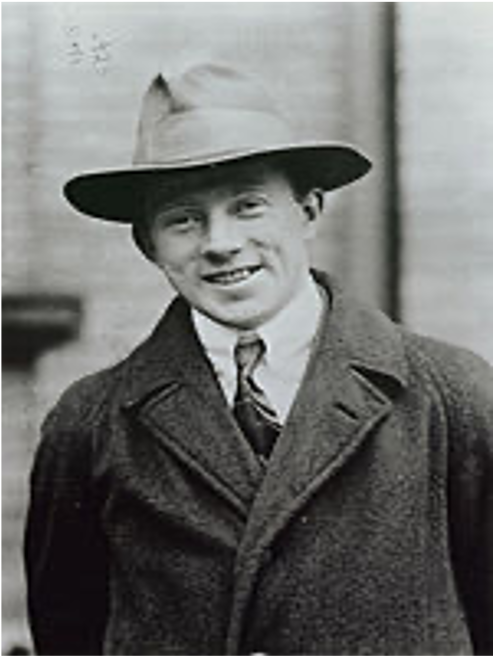
\includegraphics[width=0.25\textwidth]{figs/hesb.png}   
    \end{wrapfigure}
    维尔纳·海森堡(Werner Heisenberg,1901年12月5日-1976年2月1日),德国物理学家,1932年诺贝尔物理学奖。主要贡献:(1) 创立矩阵力学(量子力学的矩阵形式);(2)提出“测不准原理”;(3)散射(S)矩阵。  
\end{frame}

\begin{frame}
    \frametitle{}
    \begin{center}
    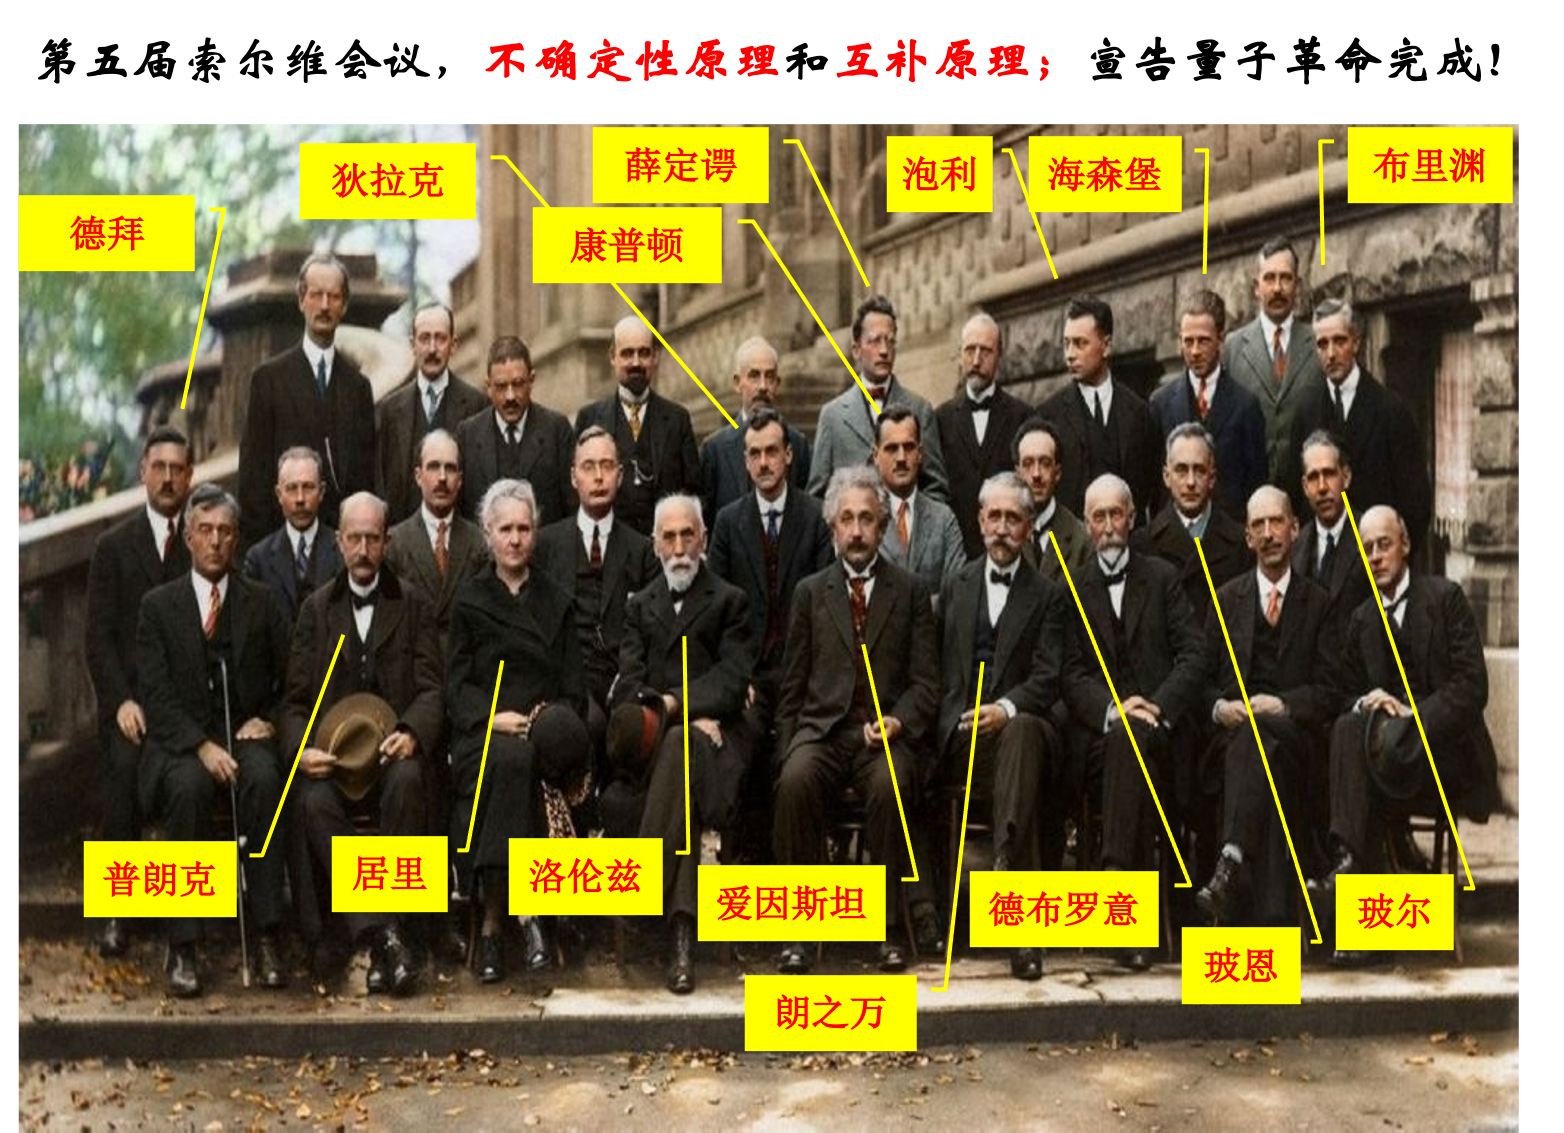
\includegraphics[width=0.8\textwidth]{figs/uncert.png}
    \end{center}
\end{frame}


\begin{frame} [allowframebreaks=]
    \begin{tcolorbox}[colback=yellow!5,colframe=yellow!75!black,title=不确定性关系式的理解]
    \begin{itemize}
        \item 若两个力学量算符不对易(对易子不等于零),对易子平均值的平方一般大于零,则它们的不确定度的积必大于零,说明它们一般不能同时具有确定值
        \item 若两个力学量算符对易,则总可以找出这样的态(比如共同的本征态),使它们同时有确定值。 
    \end{itemize}   
    \end{tcolorbox}
\end{frame} 

\begin{frame} [allowframebreaks=]
    TIPS:下列说法,正确的有:
    \begin{enumerate}
        \item 两力学量算符对易,则同时有确定值。 
        \item 两力学量算符不对易,则不能同时有确定值 
        \item 若两力学量算符有共同的本征态,则彼此对易
        \item 若两力学量算符不对易,则没有共同本征态
        \item 若[A,B]=常数,则A和B能有共同本征态
    \end{enumerate} 
\end{frame} 

\begin{frame} [allowframebreaks=]
    \frametitle{}
    \begin{tcolorbox}[colback=yellow!5,colframe=yellow!75!black,title=课堂作业]
    已知$[L_x, L_y]=i\hbar L_z$, 试计算体系处于$L_z$基态($Y_{00}=\frac{1}{\sqrt{4\pi}}$)时,$L_x, L_y$的不确定度。
    \end{tcolorbox}
\end{frame} 

  %  
%%%%%%%%%%%%%%%%%%%%%%%%%%%%%%%%%%%%%%%%%%%
\begin{frame}
    \frametitle{}
    \begin{center}
    { {\huge 第十一讲、对称与守恒量}}
    \end{center}    
\end{frame}
%%%%%%%%%%%%%%%%%%%%%%%%%%%%%%%%%%%%%


\section{前情回顾}

\begin{frame}
    \frametitle{前情回顾}
    \begin{itemize}
        \item 希尔伯特空间的态矢量描述体系状态
        \item 希尔伯特空间的算符给出体系的物理量
        \item 算符的本征函数系构成正交归一完全基
        \item 常见算符本征方程求解
        \item 算符对易关系及其物理含义 
    \end{itemize}   
\end{frame} 

\section{守恒量}

\begin{frame}
\includegraphics[width=0.6\textwidth]{figs/2021-12-17-21-25-13.png} \\
1918年 德国数学家 A. E. Noether : 从自然界的每一对称性可
得到一守恒律;反之,每一个守恒律均揭示蕴含其中的一种对称性。
\end{frame} 

\begin{frame} 
    \frametitle{守恒量定义}
    \begin{enumerate}
        \item  经典物理中的守恒量与对称条件\\
                守恒量:力学量的值不随时间变化\\
                \begin{itemize}
                    \item 机械能空间平移不变→动量守恒
                    \item 机械能空间转动不变→角动量守恒
                    \item 机械能时间平移不变→能量守恒
                \end{itemize}
        \item  量子力学中的守恒量\\
                守恒量:在任意态下力学量的平均值不随时间变化\\
                $$ \bar{F}(t)=(\Psi(t), F\Psi(t)) =c.  $$
                守恒量及守恒条件... 
    \end{enumerate}
\end{frame} 

\begin{frame} [allowframebreaks=]
    \frametitle{算符运动方程}    
        \begin{equation*}
            \begin{split} 
            \bar{F}(t)&=(\Psi(t), F(t)\Psi(t)) \\
            \frac{d\bar{F}}{dt}&=(\frac{\partial\Psi }{\partial t}, F\Psi) +(\Psi, \frac{\partial F }{\partial t}\Psi) +(\Psi, F\frac{\partial\Psi }{\partial t}) \\
            &= - \frac{1}{i\hbar} (H\Psi, F\Psi)+(\Psi, \frac{\partial F }{\partial t}\Psi) + \frac{1}{i\hbar} (\Psi, FH\Psi) \\
            &= - \frac{1}{i\hbar} (\Psi, HF\Psi)+(\Psi, \frac{\partial F }{\partial t}\Psi) + \frac{1}{i\hbar} (\Psi, FH\Psi) \\
            &= (\Psi, \frac{\partial F }{\partial t}\Psi)  +\frac{1}{i\hbar} (\Psi, [F,H]\Psi) \\
            &=\overline{(\frac{\partial F }{\partial t})}  +\frac{1}{i\hbar} \overline{[F,H]} \\
            \end{split}  
        \end{equation*}  
\end{frame} 

\begin{frame} [allowframebreaks=]
        \frametitle{力学量守恒条件} 
        由守恒量定义:   
        $$ \bar{F}(t)=(\Psi(t), F\Psi(t)) =c.  $$
        $$\frac{d\bar{F}}{dt}=\overline{(\frac{\partial F }{\partial t})}  +\frac{1}{i\hbar} \overline{[F,H]}=0$$
        得守恒量条件:
        $$\left\{\begin{aligned}
            &\frac{\partial F }{\partial t}=0\\
            &[F,H]=0 \\
        \end{aligned} \right. $$
\end{frame}

\begin{frame} 
    \frametitle{守恒量性质} 
    \begin{tcolorbox}[colback=yellow!5,colframe=yellow!75!black,title=性质1:]
        守恒量测量值概率分布不随时间改变
    \end{tcolorbox}
    \alert{证明:} F是守恒量,则 $[F,H]=0$, 设F,H的共同本征函数系$\{\varphi_n\}$, 有:\\ 
    任意态$\Psi(t)$在$\{\varphi_n\}$展开,其展开系数为:
    $$C_n(t)=(\varphi_n, \Psi(t))$$
    展开系数的模方即为测量值为本征值$f_n$的概率,因此要证明:
    $$\frac{d}{dt} |C_n(t)|^2=0$$
\end{frame}

\begin{frame} [allowframebreaks=]
    $$\begin{aligned}
      \frac{d}{dt} |C_n(t)|^2 &= \frac{d}{dt} C_n^* C_n \\
      &=C_n \frac{d}{dt} C_n^*  +  C_n^*\frac{d}{dt}C_n \\
      &=[C_n^*[\frac{d}{dt} C_n]^*  +  [C_n^*\frac{d}{dt}C_n] \\
    \end{aligned}$$
    $$\begin{aligned}
      C_n^*\frac{d}{dt}C_n&= (\varphi_n, \Psi)^* \frac{d}{dt}(\varphi_n, \Psi) \\
      &= (\varphi_n, \Psi)^* (\varphi_n, \frac{d}{dt}\Psi) \\
      &= \frac{1}{i\hbar}(\varphi_n, \Psi)^* (\varphi_n, H\Psi) \\
      &= \frac{1}{i\hbar}(\varphi_n, \Psi)^* (H\varphi_n, \Psi) \\
      &= \frac{E_n}{i\hbar}C_n ^* C_n \\
    \end{aligned}$$
    $$\begin{aligned}
        \frac{d}{dt} |C_n(t)|^2 &= [C_n^*[\frac{d}{dt} C_n]^*  +  [C_n^*\frac{d}{dt}C_n] \\
        &= [\frac{E_n}{i\hbar}C_n ^* C_n ]^* + \frac{E_n}{i\hbar}C_n ^* C_n \\
        &= -\frac{E_n}{i\hbar}C_n ^* C_n ] + \frac{E_n}{i\hbar}C_n ^* C_n \\
        &=0
    \end{aligned}$$
      证毕!
    \begin{tcolorbox}[colback=yellow!5,colframe=red!75!black,title=结论:]
        无论体系本征态还是叠加态(任意态),守恒量的平均值及各测量值的概率分布都不随时间变化。         
    \end{tcolorbox}
\end{frame}

\begin{frame} [allowframebreaks=]
    \frametitle{} 
    \begin{tcolorbox}[colback=yellow!5,colframe=yellow!75!black,title=性质2:]
        若体系有两个不对易守恒量,则一般存在简并能级
    \end{tcolorbox}
    \alert{证明:} 设F、G都是体系的守恒量,则有 $[F,H]=0$, $[G,H]=0$, 设F,H的共同本征函数系$\{\varphi_n\}$, 有:\\ 
    $$F\varphi_n =f_n \varphi_n, \qquad H\varphi_n =E_n \varphi_n $$
    $$H(G\varphi_n) =HG\varphi_n=GH\varphi_n= E_n (G\varphi_n)$$
    说明 $G\varphi_n$ 和 $\varphi_n$ 都是H的属于$E_n$的本征态。
    假设能级非简并,则$G\varphi_n$ 和 $\varphi_n$描述同一个态,两者最多只差一个常数因子,设为 $g_n$,有:
    $$G\varphi_n=g_n \varphi_n$$
    也就是说,$\varphi_n$也是G的本征态,即 F和G具有相同的本征函数系,即它们对易,与题设相矛盾。\\
    因此,体系必存在简并能级,$G\varphi_n$ 和 $\varphi_n$描述不同的态。
    \begin{tcolorbox}[colback=yellow!5,colframe=yellow!75!black,title=推论:]
        若体系有两个不对易守恒量,则一般存在简并能级, 非简并能级都是守恒量的本征态,简并能级中存在守恒量的一个本征态。\\
        根据能级简并,可找出体系的守恒量;根据能级不简并,可找到守恒量的本征态。
    \end{tcolorbox}
\end{frame}

\section{守恒定律}

\begin{frame} [allowframebreaks=]
    \frametitle{动量守恒} 
    \begin{tcolorbox}[colback=yellow!5,colframe=yellow!75!black,title=动量守恒:]
        试证明自由粒子的动量是守恒量                                   
    \end{tcolorbox}
    \alert{证明:} (1)自由粒子动量算符为:
    $$ \hat{\vec{p}} = -i\hbar\nabla  $$
    不显含时间,有 $$\frac{d}{dt}\hat{\vec{p}}=0$$ 
    (2), 自由粒子哈密顿算符为: $$ \hat{H} = \frac{1}{2\mu} \hat{\vec{p}}^2 $$
    $$\begin{aligned}
        [\hat{\vec{p}},\hat{H}]&= \frac{1}{2\mu}[\hat{\vec{p}}, \hat{\vec{p}}^2 ] \\
        &= 0
    \end{aligned}$$
    证毕!
\end{frame}

\begin{frame} [allowframebreaks=]
    \frametitle{} 
    \begin{tcolorbox}[colback=yellow!5,colframe=yellow!75!black,title=动量守恒:]
        空间平移不变性导致动量守恒                                
    \end{tcolorbox}
    \alert{证明:} (1)设体系沿x轴方向作一无穷小平移:
    $$ x \to x'=x+\delta x $$
    则体系的波函数变为:
    $$ \Psi \to \Psi'=T\Psi  $$
    波函数还是原来的波函数,只是做了平移变换: $$ \Psi'(x+\delta x) = \Psi(x) $$\\
    $$ T\Psi(x+\delta x) = \Psi(x) $$\\
    令 $x=x-\delta x$,有
    $$\begin{aligned}
        T\Psi(x)&= \Psi(x-\delta x) \\
        &= \Psi(x)-\delta x \frac{\partial}{\partial x}\Psi(x)+\cdots\\
        &= \Psi(x)-\delta x \frac{\partial}{\partial x}\Psi(x)+\cdots\\
        &= e^{-\delta x \frac{\partial}{\partial x}} \Psi(x)\\
    \end{aligned}$$
    得到平衡算符的具体形式为:
    $$\begin{aligned}
        T(\delta x)&= e^{-\delta x \frac{\partial}{\partial x}} \\
        &= e^{-\delta x (-i\hbar) \frac{\partial}{\partial x}\frac{1}{-i\hbar}} \\
        &= e^{-\frac{i}{\hbar}\delta x p_x } \\
    \end{aligned}$$
    推广到三维,有:
    $$ T(\delta \hat{\vec{r}})= e^{-\frac{i}{\hbar}\delta \hat{\vec{r}}\cdot \hat{\vec{p}} }  $$ 
    对于无穷小平移,有:
    $$T=1-\frac{i}{\hbar}\delta x p_x$$
    很明显,平移算符不显含时间,满足条件(1)
    (2)若有空间平移不变性,则有
    $$\begin{aligned}
        [T,H]&= 0 \\
        [1-\frac{i}{\hbar}\delta x p_x, H] &=0 \\
        [1, H]-[\frac{i}{\hbar}\delta x p_x, H]&=0 \\
        [\frac{i}{\hbar}\delta x p_x, H]&=0 \\
        [p_x, H] &=0 \\
    \end{aligned}$$
    证毕!
\end{frame}

\begin{frame} [allowframebreaks=]
    \frametitle{角动量守恒} 
    \begin{tcolorbox}[colback=yellow!5,colframe=yellow!75!black,title=动量守恒:]
        试证明在中心力场中运动粒子的角动量是守恒量                                
    \end{tcolorbox}
    \alert{证明:} (1)中心力场中的角动量:
    $$
    \left\{\begin{array}{l}
        \hat{L}_{x}=i \hbar\left[\sin \varphi \frac{\partial}{\partial \theta}+\cot \theta \cos \varphi \frac{\partial}{\partial \varphi}\right] \\
        \hat{L}_{y}=-i \hbar\left[\cos \varphi \frac{\partial}{\partial \theta}+\cot \theta \sin \varphi \frac{\partial}{\partial \varphi}\right] \\
        \hat{L}_{z}=-i \hbar \frac{\partial}{\partial \varphi}
        \end{array}\right.
    $$
    $$ \hat{L}^{2}=-\hbar^{2}\left[\frac{1}{\sin \theta} \frac{\partial}{\partial \theta}\left(\sin \theta \frac{\partial}{\partial \theta}\right)+\frac{1}{\sin ^{2} \theta} \frac{\partial^{2}}{\partial \varphi^{2}}\right] $$
    
    很明显,角动量不显含时间,满足条件(1)\\
    (2) 中心力场哈密顿算符为: 
    $$
    \hat{H}=-\frac{\hbar^{2}}{2 \mu r^{2}}\left[\frac{\partial}{\partial r}\left(r^{2} \frac{\partial}{\partial r}\right)+\frac{1}{\sin \theta} \frac{\partial}{\partial \theta}\left(\sin \theta \frac{\partial}{\partial \theta}\right)+\frac{1}{\sin ^{2} \theta} \frac{\partial^{2}}{\partial \varphi^{2}}\right]+U(r)
    $$
    $$
    \hat{H}=-\frac{\hbar^{2}}{2 \mu r^{2}} \frac{\partial}{\partial r}\left(r^{2} \frac{\partial}{\partial r}\right)+\frac{\hat{L}^{2}}{2 \mu r^{2}}+U(r)
    $$
    哈密顿算符与角动量各分量算符及角动量方均对易 因为(a)角动量都是$\theta, \varphi$ 的函数,与$r$无关,与哈密顿算符只含$r$的项对易。
    (b)角动量都与$L^2$对易。\\
    证毕!
\end{frame}

\begin{frame} [allowframebreaks=]
    \frametitle{能量守恒} 
    \begin{tcolorbox}[colback=yellow!5,colframe=yellow!75!black,title=能量守恒:]
        试证明哈密顿算符不显含时间的体系能量守恒                               
    \end{tcolorbox}
    \alert{证明:} (1)密顿算符不显含时间:
    不显含时间,有 $$\frac{d}{dt}\hat{H}=0$$ 
    (2), 密顿算符与自己对易: 
        $$ [\hat{H},\hat{H}]=0 $$
    证毕!
\end{frame}

\begin{frame} [allowframebreaks=]
    \frametitle{} 
    \begin{tcolorbox}[colback=yellow!5,colframe=yellow!75!black,title=角动量守恒:]
        试证明:具有空间旋转不变性的体系角动量守恒                               
    \end{tcolorbox}
    \begin{tcolorbox}[colback=yellow!5,colframe=yellow!75!black,title=能量守恒:]
        试证明:具有时间平移对称性的体系能量守恒                               
    \end{tcolorbox}
    \begin{tcolorbox}[colback=yellow!5,colframe=yellow!75!black,title=宇称守恒:]
        试证明:具有空间反射对称性的体系宇称守恒                             
    \end{tcolorbox}
\end{frame}

\begin{frame} [allowframebreaks=]
    \frametitle{宇称守恒} 
    \begin{tcolorbox}[colback=yellow!5,colframe=yellow!75!black,title=宇称守恒:]
        试证明若哈密顿算符空间反射不变,则宇称守恒                               
    \end{tcolorbox}
    \alert{证明:} (1)宇称算符:
    空间反射:$$\vec{r} \to -\vec{r} $$
    $$\Psi(\vec{r}) \to \Psi(-\vec{r}) $$
    定义宇称算符: $$ \hat{P}\Psi(\vec{r},t) = \Psi(-\vec{r},t) $$
    
    (2) 解宇称算符本征方程: 
    对于本征函数 $\psi_p (\vec{r})$, 有:
    $$\begin{aligned}
        \hat{P}\psi_p (\vec{r}) &= p\psi_p (\vec{r}) \\
        \hat{P}^2\psi_p (\vec{r}) &= \hat{P} p\psi_p (\vec{r}) = p^2\psi_p (\vec{r})\\
        &= 0
    \end{aligned}$$
    基于定义式,有:
    $$\begin{aligned}
        \hat{P}^2\psi_p (\vec{r}) &= \hat{P} [\hat{P} \psi_p (\vec{r})]\\
        &= \hat{P} \psi_p (-\vec{r})\\
        &= \psi_p (\vec{r})\\
    \end{aligned}$$
    得本征值 $p=\pm 1$,分别称为偶宇称和奇宇称。\\
    (3) 证明宇称守恒 \\
    (a) 显然,宇称算符不显含时间t\\
    (b) 哈密顿算符具有空间反射不变性,即:
    $$ H(\vec{r},t)= H(-\vec{r},t)$$
    对于任意态,有:
    $$\begin{aligned}
        \hat{P} (\hat{H}(\vec{r},t) \Psi (\vec{r},t)) &= \hat{H}(-\vec{r},t) \Psi (-\vec{r},t)\\
        &= \hat{H}(\vec{r},t) \Psi (-\vec{r},t)\\
        &= \hat{H}(\vec{r},t) \hat{P} \Psi (\vec{r},t)\\
    \end{aligned}$$
    得: $$ \hat{P} \hat{H} = hat{H} \hat{P} $$
    即:$$[\hat{P}, \hat{H}]=0$$
    证毕!
\end{frame}

\begin{frame}
    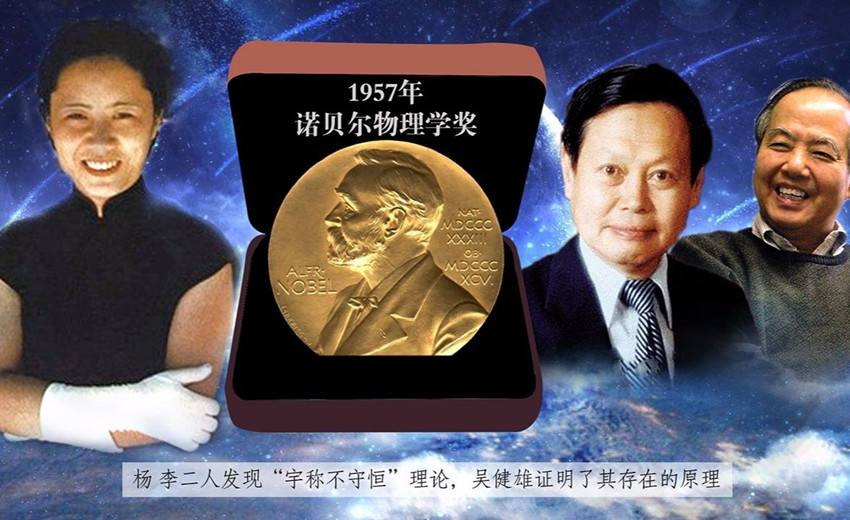
\includegraphics[width=0.8\textwidth]{figs/2021-12-18-00-23-17.png} \\
\end{frame} 





  %                     %
%%%%%%%%%%%%%%%%%%%%%%%%%%%%%%%%%%%%55%%
\begin{frame} [plain]
    \frametitle{}
    \Background[1] 
    \begin{center}
    { {\huge 第十二讲、矩阵表示 }}
    \end{center}  
    \addtocounter{framenumber}{-1}   
\end{frame}
%%%%%%%%%%%%%%%%%%%%%%%%%%%%%%%%%%

%%%%%%%%%%%%%%%%%%%%%%%%%%%%%%%%%
\begin{frame}
        \frametitle{主要内容}
        \transfade
        \tableofcontents
        \addtocounter{framenumber}{-1} 
\end{frame}
%%%%%%%%%%%%%%%%%%%%%%%%%%%%%%%%%%

\section{前情回顾}

\begin{frame}
    \frametitle{前情回顾}
    \begin{itemize}
        \item 波函数 : $$ \Psi(\vec{r},t)$$
        \item 薛定谔方程 :     
        \begin{equation*}
            i\hbar \frac{\partial }{\partial t} \Psi(\vec{r},t) = (\frac{\hbar^2}{2\mu} \nabla^2 +U(\vec{r})) \Psi(\vec{r},t)
        \end{equation*}
        \item 力学量算符 :
        $$\left\{ \begin{aligned}
            &\hat{\vec{r}} =\vec{r}  \\
            &\hat{\vec{p}} =-i\hbar(\dfrac{d}{d x}+ \dfrac{d}{d y} + \dfrac{d}{d z}) \\
            &\hat{F}=F(\hat{\vec{r}},\hat{\vec{p}}) \\
        \end{aligned} \right.$$
    \end{itemize}   
\end{frame} 

\section{表象理论}

\begin{frame} 
    \frametitle{}
    \begin{tcolorbox1}{定义:}
        \begin{itemize}
            \item 表象:波函数和力学量的具体表示形式,选择一个力学量本征函数系做为基就是选取一种表象
            \item 表象理论:研究量子力学各种表示形式以及它们之间的相互变换的理论。
            \item 矩阵表示:波函数在某个基上的展开系数构成矩阵 
        $$ \Psi(\vec{r},t)=\sum_n c_n(t) \psi_n(\vec{r})$$ 
        $$ \Psi\Leftrightarrow(c_1,c_2,\cdots)^T $$
        \end{itemize}   
    \end{tcolorbox1}
\end{frame} 

\section{波函数矩阵表示}
\begin{frame} 
    \frametitle{展开系数}    
    对于任意表象Q,若:\\
     本征分立谱: $\psi_n(\vec{r}) \to u_n(\vec{r})$, $c_n \to a_n $
        \begin{equation*}
            a_n(t)=(u_n(\vec{r}), \Psi(\vec{r},t)) 
        \end{equation*}  
    本征连续谱: $\psi_n(\vec{r}) \to u_q(\vec{r})$, $c_n \to a(q) $
        \begin{equation*}
            a(q,t)=(u_q(\vec{r}), \Psi(\vec{r},t)) 
        \end{equation*}  
\end{frame} 

\begin{frame} 
        \frametitle{1、波函数矩阵表示} 
        \begin{equation*}
            \begin{split} 
                \Psi(\vec{r},t)&=\sum_n a_n(t) u_n(\vec{r}) \\
                &=a_1(t) u_1+ a_2(t) u_2+\cdots+ a_n(t) u_n \\
                &=(u_1,u_2,\cdots,u_n) 
               \begin{pmatrix}
                    a_1(t)\\
                    a_2(t)\\
                    \cdots\\
                    a_n(t)
                \end{pmatrix} \\
                &= (u_1,u_2,\cdots,u_n) (a_1(t),a_2(t),\cdots, a_n(t))^T
            \end{split}  
        \end{equation*}  
        因此,有: $$   \Psi \Leftrightarrow (a_1(t),a_2(t),\cdots, a_n(t))^T \Leftrightarrow {\color{red}  \pmb {\Psi} } $$
\end{frame}

\begin{frame} 
    \frametitle{对比} 
    $$\begin{matrix}
      ~~  & \text{矢量空间} & \text{希尔伯特空间}\\ \vspace{0.6em}
      \text{基}  & \{\vec{e}_1,\vec{e}_2,\vec{e}_3\}  & \{ u_1,u_2,\cdots,u_n \}\\ \vspace{0.6em}
      \text{正交归一}  & \vec{e}_i \cdot \vec{e}_j=\delta_{ij} & ( u_m, u_n)= \delta_{mn}\\ \vspace{0.6em}
      \text{完备性}  & \vec{P}=\sum\limits_{i=1}^{3} x_i \vec{e}_i &  \Psi=\sum_n a_n(t) u_n \\  \vspace{0.6em}
      \text{投影}  & x_i= \vec{e}_i \cdot \vec{P}  & a_n(t)=( u_m, \Psi) \\ \vspace{0.6em}
      \text{矩阵}  & (x_1, x_2, x_3)^T & (a_1(t), a_2(t), \cdots, a_n(t))^T
      \end{matrix}
      $$
\end{frame}

\begin{frame} 
    \frametitle{实例} 
    \begin{tcolorbox2}{例1:}
        求动量本征态(平面波)在动量表象中的具体形式(矩阵表示)
    \end{tcolorbox2}
    \alert{解:} 动量的本征谱连续,采用公式\\
    $$a(q,t)=(u_q(\vec{r}), \Psi(\vec{r},t)) $$
    取 $$u_q(\vec{r})=\psi_{\vec{p}}(\vec{r})=\frac{1}{(2\pi\hbar)^{3/2}}e^{\frac{i}{\hbar}\vec{p}\cdot \vec{r}}, 
    \qquad \Psi(\vec{r},t))=\frac{1}{(2\pi \hbar)^{3/2}} e^{\frac{i}{\hbar}(\vec p\cdot \vec r -Et)} = 
    \psi_{\vec{p}'}e^{-\frac{i}{\hbar}Et}  $$
\end{frame}

\begin{frame} [allowframebreaks=]
    \frametitle{}
    \begin{equation*}
        \begin{split}
            a(q,t)&=(u_q(\vec{r}), \Psi(\vec{r},t)) \\
            a(p,t)&= (\psi_{\vec{p}}(\vec{r}), \psi_{\vec{p}'}e^{-\frac{i}{\hbar}Et})\\
            &= e^{-\frac{i}{\hbar}Et}(\psi_{\vec{p}}(\vec{r}), \psi_{\vec{p}'})\\
            &= e^{-\frac{i}{\hbar}Et}\delta(\vec{p}-\vec{p}')\\
        \end{split} 
    \end{equation*}
    \begin{tcolorbox}[colback=yellow!5,colframe=yellow!75!black,title=TIPS:]
        本征态在自身表象中的矩阵表示为$\delta$函数。
    \end{tcolorbox}
\end{frame} 

\begin{frame} [allowframebreaks=]
    \begin{tcolorbox2}{例2:}
        如下波函数是某体系的能量本征态\\
        $$ \psi_n(x)=\sqrt{\frac{2}{a}} \sin \frac{n\pi}{a}x, \qquad 0<x<a $$
        求基态(n=1)分别在动量和能量表象中的具体形式
    \end{tcolorbox2}
    \alert{解:} (1)动量的本征谱连续,采用公式\\
    \begin{equation*}
        \begin{split}
            a(q,t)&=(u_q(\vec{r}), \Psi(\vec{r},t)) \\
            a(p)&= (\psi_{p}(x), \psi_1(x))\\
            &= (\frac{1}{\sqrt{2\pi\hbar}}e^{\frac{i}{\hbar}px}, \sqrt{\frac{2}{a}} \sin \frac{\pi}{a}x)
        \end{split} 
    \end{equation*}

    \begin{equation*}
        \begin{split}
          ~~~~~~&= \frac{1}{\sqrt{2\pi\hbar}}\sqrt{\frac{2}{a}} (e^{\frac{i}{\hbar}px},  \sin \frac{\pi}{a}x)\\
            &= \frac{1}{\sqrt{2\pi\hbar}}\sqrt{\frac{2}{a}} \int_0 ^a e^{{\color{red}-}\frac{i}{\hbar}px}\sin \frac{\pi}{a}x) dx\\
            &=\sqrt{\frac{a\pi}{\hbar}} \frac{1+e^{\frac{i}{\hbar}pa}}{\pi^2-p^2a^2/\hbar^2}
        \end{split} 
    \end{equation*}

    (2)能量本征谱分立,采用公式\\
    \begin{equation*}
        \begin{split}
            a_n(t)&=(u_n(\vec{r}), \Psi(\vec{r},t)) \\
            a_{E_n}&=(\psi_n(x), \psi_1(x)) \\
            &=\delta_{1n} \\
        \end{split} 
    \end{equation*}  
\end{frame} 

\section{算符矩阵表示}
\begin{frame} [allowframebreaks=]
    \frametitle{2、算符矩阵表示}    
    算符有如下定义式:
    \begin{equation*}
        \varphi(\vec{r})=F\Psi(\vec{r}) 
    \end{equation*}  
    把两波函数在任意表象Q中展开 (基$u_n(\vec{r})$):\\
    \begin{equation*}
        \begin{split} 
         \sum_m b_m(t)u_m(\vec{r})&= F\sum_m a_m(t)u_m(\vec{r}) \\
         \sum_m b_m(t)u_m(\vec{r})&= \sum_m Fu_m(\vec{r})a_m(t) \\
         \sum_m b_m(t)u_n ^*(\vec{r}) u_m(\vec{r})&= \sum_m u_n ^*(\vec{r}) Fu_m(\vec{r})a_m(t) \\
         \sum_m b_m(t)(u_n (\vec{r}), u_m(\vec{r}))&= \sum_m (u_n (\vec{r}), Fu_m(\vec{r}))a_m(t) \\
         \sum_m b_m(t)\delta_{nm}&= \sum_m (u_n (\vec{r}), Fu_m(\vec{r}))a_m(t) \\
        \end{split}  
    \end{equation*} 
    \begin{equation*}
        \begin{split} 
         \sum_m b_m(t)\delta_{nm}&= \sum_m (u_n (\vec{r}), Fu_m(\vec{r}))a_m(t) \\
         b_n(t)&= \sum_m (u_n (\vec{r}), Fu_m(\vec{r}))a_m(t) \\
         b_n(t)&= \sum_m F_{nm} a_m(t) 
        \end{split}  
    \end{equation*} 
    取遍$n, m$, 得到如下矩阵形式\\
    $$\begin{pmatrix}
        b_1(t)\\
        b_2(t)\\
        \cdots \\
        b_n(t)
    \end{pmatrix}
    =
    \begin{pmatrix}
       F_{11} & F_{12} & \cdots & F_{1n} \\
       F_{21} & F_{22} & \cdots & F_{2n} \\
       \cdots & \cdots &  \cdots& \cdots\\
        F_{n1} & F_{n2} & \cdots & F_{nn} \\
    \end{pmatrix}
    \begin{pmatrix}
        a_1(t)\\
        a_2(t)\\
        \cdots \\
        a_n(t)
    \end{pmatrix}
    $$
    算符矩阵元公式: $$ F_{nm}=(u_n (\vec{r}), Fu_m(\vec{r})) $$
\end{frame} 

\section{算符矩阵表示的性质}
\begin{frame} 
    \frametitle{3、算符矩阵性质} 
    \begin{enumerate}
    \item  力学量算符的矩阵是厄密矩阵 
    \item  力学量算符的矩阵,对角元都是实数
    \item  力学量算符在自身表象是对角矩阵,对角元素就是算符的本征值
    \end{enumerate}
\end{frame}

\begin{frame} 
    \frametitle{定义} 
    \begin{tcolorbox1}{定义:}
        \begin{itemize}
        \item F的共轭矩阵: $F^{\dagger } =(F^*)^T$
        \item 厄密矩阵: $F= F^{\dagger }$
        \end{itemize}
    TIPS:厄密矩阵矩阵元特点 $$  F_{nm}^* = F_{mn}  $$
    \end{tcolorbox1}
\end{frame}

\begin{frame} 
    \frametitle{} 
    下列矩阵,哪些是厄密矩阵\\
    $$\begin{matrix}
        \begin{pmatrix}
            a & 0 & 0 & 0 \\
            0 & b & 0 & 0 \\
            0 & 0 & c & 0\\
            0 & 0 & 0 & 0 \\
         \end{pmatrix} 
         &  
         \begin{pmatrix}
            a & 1 & 0 & 0 \\
            2 & b & 0 & 0 \\
            0 & 0 & c & 0\\
            0 & 0 & 0 & 0 \\
         \end{pmatrix} 
         & 
         \begin{pmatrix}
            a & 1 & 0 & 0 \\
            1 & b & 0 & 0 \\
            0 & 0 & c & 0 \\
            0 & 0 & 0 & 0 \\
         \end{pmatrix} 
         \\ \vspace{0.6em}
         \begin{pmatrix}
            a & 1 & 0 & 0 \\
            -1 & b & 0 & 0 \\
            0 & 0 & c & 0 \\
            0 & 0 & 0 & 0 \\
         \end{pmatrix} 
         &     
        \begin{pmatrix}
            a & i & 0 & 0 \\
            i & b & 0 & 0 \\
            0 & 0 & c & 0 \\
            0 & 0 & 0 & 0 \\
        \end{pmatrix} 
         &   
         \begin{pmatrix}
            a & -i & 0 & 0 \\
            i & b & 0 & 0 \\
            0 & 0 & c & 0 \\
            0 & 0 & 0 & 0 \\
         \end{pmatrix} 
    \end{matrix}
        $$
\end{frame}


\begin{frame} [allowframebreaks=]
    \begin{tcolorbox1}{性质1:}
        试证明力学量算符的矩阵表示都是厄密矩阵
    \end{tcolorbox1}
    \alert{证明:} 
    \begin{equation*}
        \begin{split}
            F_{nm}&=(u_n (\vec{r}), Fu_m(\vec{r}))\\
            &=(Fu_n (\vec{r}), u_m(\vec{r}))\\
            &=(u_m(\vec{r}), Fu_n (\vec{r}))^*\\
            &=F_{mn}^*\\
        \end{split} 
    \end{equation*}
    证毕!
\end{frame}

\begin{frame} [allowframebreaks=]
    \begin{tcolorbox1}{性质2:}
        试证明力学量算符的矩阵表示,其对角元都是实数
    \end{tcolorbox1}
    \alert{证明:} 
    \begin{equation*}
        \begin{split}
            F_{nm}&=F_{mn}^*\\
            F_{nn}&=F_{nn}^*\\
        \end{split} 
    \end{equation*}
    即:对角元都是实数。 \\
    证毕!
\end{frame}

\begin{frame} [allowframebreaks=]
    \begin{tcolorbox1}{性质3:}
        试证明力学量算符的矩阵表示,在自身表象中是对角矩阵
    \end{tcolorbox1}
    \alert{证明:} 
    \begin{equation*}
        \begin{split}
            F_{nm}&=(u_n (\vec{r}), Fu_m(\vec{r}))\\
            &=(u_n (\vec{r}), f_nu_m(\vec{r}))\\
            &=f_n(u_n (\vec{r}), u_m(\vec{r}))\\
            &=f_n\delta_{mn}\\
        \end{split} 
    \end{equation*}
    即:(1)非对角元都是0,是对称阵。(2)对角元就是本征值\\
    证毕!
\end{frame}

\begin{frame} [allowframebreaks=]
    \begin{tcolorbox2}{对角化的物理意义}
        \begin{itemize}
            \item 力学量算符的表示一般不是对称阵(不在自身表象)
            \item 在数学上做矩阵对角化,使其成为对角阵 (在自身表象)
            \item 对角化完成从任意表象回到自身表象的过程
            \item 对角元就是本征值(解本征方程求本征值)
        \end{itemize}  
    \end{tcolorbox2}
\end{frame}

\begin{frame} 
    \frametitle{}
    \begin{tcolorbox2}{课堂作业:}
    取Q表象为动量表象,试求位置算符$\hat{x}$、动量算符$\hat{p}_x$ 的具体形式。
    \end{tcolorbox2}
\end{frame} 

\begin{frame} 
    \frametitle{}
    \begin{tcolorbox2}{课堂讨论}
    已知波函数取如下形式:$$\psi(x)=\dfrac{1}{\sqrt{2}}u_1(x)+\dfrac{1}{2}u_2(x)+\dfrac{1}{2}u_3(x)$$
    其系数矩阵为$$\begin{pmatrix}
            \dfrac{1}{\sqrt{2}}\\
            \dfrac{1}{2}\\
            \dfrac{1}{2}
            \end{pmatrix}$$
    \begin{enumerate}
        \item  此系数矩阵是波函数在位置表象的矩阵表示吗?
        \item  此系数矩阵是波函数在能量表象的矩阵表示的条件是什么?  
    \end{enumerate}
    \end{tcolorbox2}
\end{frame} 

  % 
%%%%%%%%%%%%%%%%%%%%%%%%%%%%%%%%%%%%55%%
\begin{frame} [plain]
    \frametitle{}
    \Background[1] 
    \begin{center}
    { {\huge 第十三讲、量子力学公式的矩阵化 }}
    \end{center}  
    \addtocounter{framenumber}{-1}   
\end{frame}
%%%%%%%%%%%%%%%%%%%%%%%%%%%%%%%%%%

%%%%%%%%%%%%%%%%%%%%%%%%%%%%%%%%%
\begin{frame}
        \frametitle{主要内容}
        \transfade
        \tableofcontents
        \addtocounter{framenumber}{-1} 
\end{frame}
%%%%%%%%%%%%%%%%%%%%%%%%%%%%%%%%%%

\section{前情回顾}


\begin{frame}
    \frametitle{前情回顾}
    \begin{itemize}
       \done 波函数矩阵表示 :$$ a_n(t)=(u_n(\vec{r}), \Psi(\vec{r},t)) $$ 
       \done 力学量算符矩阵表示 : $$ F_{nm}=(u_n (\vec{r}), Fu_m(\vec{r})) $$   
       \todo 公式的矩阵化:$\cdots$
    \end{itemize}
\end{frame} 



\begin{frame} 
    \frametitle{}
    \begin{tcolorbox2}{量子力学常用公式}
        \begin{itemize}
            \item 平均值公式
            \item 归一化公式
            \item 本征方程
            \item 薛定谔方程
            \item 运动方程
        \end{itemize}   
    \end{tcolorbox2}
\end{frame} 

\section{平均值公式}

\begin{frame} 
    \frametitle{}
    \begin{tcolorbox1}{平均值公式}
        求平均值公式在Q表象中的具体形式(矩阵表示)
        $$ \bar{F}=\int \Psi^* (\vec{r},t) F \Psi(\vec{r},t) d\tau $$
    \end{tcolorbox1}
    \alert{解:} 
    \begin{equation*}
        \begin{split}
            \bar{F}&=(\Psi(\vec{r},t), F\Psi(\vec{r},t)) \\
            &= (\sum_n a_n(t) u_n(\vec{r}), \sum_m a_m(t) F u_m(\vec{r}))\\
            &= \sum_{n,m} a_n ^*(t) (u_n(\vec{r}), F u_m(\vec{r})) a_m(t)\\
            &= \sum_{n,m} a_n ^*(t) F_{nm} a_m(t)\\
        \end{split} 
    \end{equation*}
\end{frame}

\begin{frame} 
    取遍$n, m$, 得到如下矩阵形式\\
    $$\bar{F} =(a_1 ^*(t), a_2 ^*(t),\cdots,a_n^*(t) )
    \begin{pmatrix}
       F_{11} & F_{12} & \cdots & F_{1n} \\
       F_{21} & F_{22} & \cdots & F_{2n} \\
       \cdots & \cdots &  \cdots& \cdots\\
        F_{n1} & F_{n2} & \cdots & F_{nn} \\
    \end{pmatrix}
    \begin{pmatrix}
        a_1(t)\\
        a_2(t)\\
        \cdots \\
        a_n(t)
    \end{pmatrix}
    $$ \vspace{1.0em} 
    $$ \large \color{red} \bar{F} = \pmb {\Psi} ^{\dagger } \pmb {F} \pmb {\Psi} $$
\end{frame}

\begin{frame} 
    在自身表象中,有:
    $$\bar{F} =(a_1 ^*(t), a_2 ^*(t),\cdots,a_n^*(t) )
    \begin{pmatrix}
       f_1 & 0 & \cdots & 0 \\
       0& f_2 & \cdots & 0 \\
       \cdots & \cdots &  \cdots& \cdots\\
        0 & 0 & \cdots & f_n \\
    \end{pmatrix}
    \begin{pmatrix}
        a_1(t)\\
        a_2(t)\\
        \cdots \\
        a_n(t)
    \end{pmatrix}
    $$
    \vspace{1.0em} 
    $$ \large \color{red} \bar{F} = \sum_n a_n^*(t) a_n(t) f_n= \sum_n |a_n(t)|^2 f_n $$
\end{frame}

\section{归一化公式}

\begin{frame} 
    \frametitle{}
    \begin{tcolorbox1}{归一化公式}
        求归一化公式在Q表象中的具体形式(矩阵表示)
        $$ \int \Psi^* (\vec{r},t) \Psi(\vec{r},t) d\tau =1 $$
    \end{tcolorbox1}
    \alert{解:} 
    \begin{equation*}
        \begin{split}
            1 &=(\Psi(\vec{r},t), \Psi(\vec{r},t)) \\
            &= (\sum_n a_n(t) u_n(\vec{r}), \sum_m a_m(t) u_m(\vec{r}))\\
            &= \sum_{n,m} a_n ^*(t) (u_n(\vec{r}), u_m(\vec{r})) a_m(t)\\
            &= \sum_{n,m} a_n ^*(t) \delta_{nm} a_m(t)\\
        \end{split} 
    \end{equation*}
\end{frame}


\begin{frame} 
    $$  \sum_{n} a_n ^*(t) a_n(t) =1 $$
    取遍$n$, 得到如下矩阵形式\\
    $$ (a_1 ^*(t), a_2 ^*(t),\cdots,a_n^*(t) )
    \begin{pmatrix}
        a_1(t)\\
        a_2(t)\\
        \cdots \\
        a_n(t)
    \end{pmatrix}
    =1 $$ \vspace{1.0em} 
    $$ \large \color{red} \pmb {\Psi} ^{\dagger } \pmb {\Psi} =1 $$

\end{frame}

\section{本征方程}

\begin{frame} 
    \frametitle{}
    \begin{tcolorbox1}{3、本征方程}
        求本征方程在Q表象中的具体形式(矩阵表示)
        $$ F\psi_n (\vec{r}) =f \psi_n (\vec{r})$$
    \end{tcolorbox1}
    \alert{解:} 
    \begin{equation*}
        \begin{split}
            F\psi_m (\vec{r}) &=f \psi_m \\
            \psi_n ^*  F\psi_m &=\psi_n ^* f \psi_m\\
            (\psi_n, F\psi_m )&=(\psi_n, f \psi_m)\\
            (\psi_n, F\psi_m )&=(\psi_n, f \psi_m)\\
            F_{nm} &=f_m \delta_{nm}
        \end{split} 
    \end{equation*}
\end{frame}

\begin{frame} 
    $$ \sum_n (F_{nm} -f \delta_{nm})a_n=0 $$
    取遍$n,m$, 得矩阵形式\\            
    $$\begin{pmatrix}
        F_{11}-f & F_{12} & \cdots & F_{1n} \\
        F_{21} & F_{22}-f & \cdots & F_{2n} \\
        \cdots & \cdots &  \cdots& \cdots\\
         F_{n1} & F_{n2} & \cdots & F_{nn}-f \\
     \end{pmatrix}
     \begin{pmatrix}
         a_1(t)\\
         a_2(t)\\
         \cdots \\
         a_n(t)
     \end{pmatrix}
     =0 \qquad (1)$$
     $$ \color{red} (\pmb F -f \pmb I) \pmb \Psi =0 $$

    有解条件,系数行列式等于零!
\end{frame}

\begin{frame} 
    得久期方程:
    $$\begin{vmatrix}
        F_{11}-f & F_{12} & \cdots & F_{1n} \\
        F_{21} & F_{22}-f & \cdots & F_{2n} \\
        \cdots & \cdots &  \cdots& \cdots\\
         F_{n1} & F_{n2} & \cdots & F_{nn}-f \\
     \end{vmatrix} 
     =0 \qquad (2) $$
     解久期方程, 得本征谱{$f_1,f_2,\cdots, f_n $}\\
     依次把$f_i$ 代回方程(1),解得第i个本征函数。本征方程得解\\
     矩阵化使本征方程从微分方程变为代数方程!
\end{frame}

\begin{frame} 
    \begin{tcolorbox2}{例1:}
        已知算符在Q表象中的矩阵形式如下。
        $$ L_x= \frac{\hbar}{\sqrt{2}}
        \begin{pmatrix}
            0 & 1 & 0  \\
            1 & 0 & 1  \\
            0 & 1 & 0 \\
         \end{pmatrix} $$
        求本征值和归一化本征函数,并将矩阵对角化。
    \end{tcolorbox2}
    可选方案:
    \begin{itemize}
        \done 解久期方程,得本征值,然后代入方程(1),得本征函数 ,再直接写出对角阵 
        \todo 直接从数学上对角化,对角元就是本征值,然后代入方程(1),得本征函数。
     \end{itemize}
\end{frame}

\begin{frame} 
    \alert{解:}第一步:解久期方程求本征值
    $$\frac{\hbar}{\sqrt{2}}
    \begin{vmatrix}
       0-f & 1 & 0  \\
       1 & 0-f & 1  \\
       0 & 1 & 0-f \\
    \end{vmatrix} 
    =0 \qquad (2) $$
   $$ -f^3+2f=0 $$
   $$ f_1=\sqrt{2}, f_2=0, f_3=-\sqrt{2} $$
   注意:这只是
   $$\begin{pmatrix}
       0 & 1 & 0  \\
       1 & 0 & 1  \\
       0 & 1 & 0 \\
    \end{pmatrix} $$
    的本征值,$L_x$的本征值为 $\lambda_i=\dfrac{\hbar}{\sqrt{2}} f_i$,即 $ \hbar, 0, -\hbar$
\end{frame}

\begin{frame} 
    第二步:把$f_i$ 代回方程(1)求本征函数
    $$\begin{pmatrix}
        0-f & 1 & 0  \\
        1 & 0-f & 1  \\
        0 & 1 & 0-f \\
     \end{pmatrix} 
     \begin{pmatrix}
         a_1\\
         a_2\\
         a_3
     \end{pmatrix}
     =0 \qquad (1)$$

     $$\begin{matrix}
       f_1=\sqrt{2} & f_2=0  &  f_3=-\sqrt{2}\\
    \begin{pmatrix}
        1/\sqrt{2}a_2\\
        a_2\\
        1/\sqrt{2}a_2
    \end{pmatrix}  
    = 1/\sqrt{2}a_2 \begin{pmatrix}
        1\\
        \sqrt{2}\\
        1
        \end{pmatrix} 
    & 
    \begin{pmatrix}
        a_1\\
        0\\
        a_1
    \end{pmatrix}  
    =  a_1 \begin{pmatrix}
        1\\
        0\\
        1
    \end{pmatrix}
    &
    \begin{pmatrix}
        -1/\sqrt{2}a_2\\
        a_2\\
        -1/\sqrt{2}a_2
    \end{pmatrix} 
    = 1/\sqrt{2}a_2 \begin{pmatrix}
        -1\\
        \sqrt{2}\\
        -1
    \end{pmatrix} 
    \end{matrix}$$           
\end{frame}


\begin{frame} 
    代入归一化公式, $$ \pmb {\Psi} ^{\dagger } \pmb {\Psi} =1 $$

    $$\begin{matrix}
    f_1=\sqrt{2} & f_2=0  &  f_3=-\sqrt{2}\\
    \dfrac{1}{2} a_2 ^2 (1, \sqrt{2}, 1)
    \begin{pmatrix}
    1\\
    {\sqrt{2}}\\
    1
    \end{pmatrix} 
    =1 
    & 
    a_1 ^2 (1, 0, 1)
    \begin{pmatrix}
     1\\
     0\\
     1
    \end{pmatrix} 
    =1 
     &
     \dfrac{1}{2} a_2 ^2 (-1, \sqrt{2}, -1)
    \begin{pmatrix}
     -1\\
     {\sqrt{2}}\\
     -1
    \end{pmatrix} 
    =1 \\
    a_2= \dfrac{1}{\sqrt{2}} &  a_1= \dfrac{1}{\sqrt{2}} &   a_2=\dfrac{1}{\sqrt{2}} 
    \\
    \psi_1=\dfrac{1}{2}
    \begin{pmatrix}
    1\\
    \sqrt{2}\\
    1
    \end{pmatrix}  
    & 
    \psi_2=\dfrac{1}{\sqrt{2}}
    \begin{pmatrix}
    1\\
    0\\
    1
    \end{pmatrix}  
    &
    \psi_3=\dfrac{1}{2}
    \begin{pmatrix}
    -1\\
    \sqrt{2}\\
    -1
    \end{pmatrix}  
    \end{matrix}$$   
\end{frame}

\begin{frame} 
    第三步:写出对角阵:
    $$ L_x= \frac{\hbar}{\sqrt{2}}
        \begin{pmatrix}
            0 & 1 & 0  \\
            1 & 0 & 1  \\
            0 & 1 & 0 \\
         \end{pmatrix} 
    = 
    \begin{pmatrix}
        \hbar & 0 & 0  \\
        0 & 0 &   \\
        0 & 0 & -\hbar \\
     \end{pmatrix} 
    $$
\end{frame}

\section{薛定谔方程}
\begin{frame} 
    \frametitle{}
    \begin{tcolorbox1}{4、薛定谔方程}
        求薛定谔方程在Q表象中的具体形式(矩阵表示)
        $$ i\hbar \frac{\partial}{\partial t }\psi (\vec{r},t) =H\psi (\vec{r},t)$$
    \end{tcolorbox1}
    \alert{解:} 波函数在Q表象展开
    \begin{equation*}
        \begin{split}
            i\hbar \frac{\partial}{\partial t }\sum_n a_n(t) u_n(\vec{r})  &=H\sum_n a_n(t) u_n(\vec{r}) \\
            u_m ^* (\vec{r}) i\hbar \frac{\partial}{\partial t }\sum_n a_n(t) u_n(\vec{r})  &=u_m ^* (\vec{r})H\sum_n a_n(t) u_n(\vec{r}) \\
            i\hbar \frac{\partial}{\partial t }u_m ^* (\vec{r}) \sum_n a_n(t) u_n(\vec{r})  &=u_m ^* (\vec{r})\sum_n a_n(t) Hu_n(\vec{r}) \\      
        \end{split} 
    \end{equation*}
\end{frame}

\begin{frame} 
    \begin{equation*}
        \begin{split}
            i\hbar \frac{\partial}{\partial t }(u_m (\vec{r}), \sum_n a_n(t) u_n(\vec{r}) ) &=(u_m (\vec{r}), \sum_n a_n(t) Hu_n(\vec{r})) \\
            i\hbar \frac{\partial}{\partial t }\sum_n a_n(t)(u_m (\vec{r}),  u_n(\vec{r}) ) &=\sum_n (u_m (\vec{r}),  Hu_n(\vec{r}))a_n(t) \\
            i\hbar \frac{\partial}{\partial t }\sum_n a_n(t)\delta_{mn} &=\sum_n  H_{mn} a_n(t) \\
            i\hbar \frac{\partial}{\partial t } a_n(t) &=\sum_n H_{mn} a_n(t)  \\
        \end{split} 
    \end{equation*}
\end{frame}

\begin{frame} 
    取遍$n,m$, 得矩阵形式\\ 
    $$i\hbar \frac{\partial}{\partial t }  
    \begin{pmatrix}
        a_1(t)\\
        a_2(t)\\
        \cdots \\
        a_n(t)
    \end{pmatrix}
    =         
    \begin{pmatrix}
        H_{11} & H_{12} & \cdots & H_{1n} \\
        H_{21} & H_{22} & \cdots & H_{2n} \\
        \cdots & \cdots &  \cdots& \cdots\\
        H_{n1} & F_{n2} & \cdots & H_{nn} \\
     \end{pmatrix}
     \begin{pmatrix}
         a_1(t)\\
         a_2(t)\\
         \cdots \\
         a_n(t)
     \end{pmatrix}
    $$ \vspace{0.6em }
    $$\color{red} i\hbar \frac{\partial}{\partial t }  \pmb \Psi = \pmb H  \pmb \Psi $$
\end{frame}

\section{算符运动方程}
\begin{frame} 
    \frametitle{}
    \begin{tcolorbox1}{5、算符运动方程}
        求运动方程在Q表象中的具体形式(矩阵表示)
        $$ \frac{d\overline{F}}{dt}=\overline{\frac{\partial F }{\partial t}}  +\frac{1}{i\hbar} \overline{[F,H]}$$
    \end{tcolorbox1}
    \alert{解:} 波函数在Q表象展
    \begin{equation*}
        \begin{split}
            \frac{d(\psi,F \psi )}{dt} &=(\psi,\frac{\partial F }{\partial t} \psi)  +\frac{1}{i\hbar}  ( \psi,[F,H]\psi) \\
            \frac{d(\sum_m a_m u_m,F \sum_n a_n u_n )}{dt} &=(\sum_m a_m u_m,\frac{\partial F }{\partial t} \sum_n a_n u_n) \\  
            &+\frac{1}{i\hbar}  (\sum_m a_m u_m,[F,H]\sum_n a_n u_n)  \\    
        \end{split} 
    \end{equation*}
\end{frame}

\begin{frame} 
    \begin{equation*}
        \begin{split}
            \frac{d\sum_{mn}a_m ^* (u_m,Fu_n )a_n}{dt} &=\sum_{mn} a_m ^*  (u_m,\frac{\partial F }{\partial t} u_n)a_n \\  
            &+\frac{1}{i\hbar} \sum_{mn} a_m ^*  ( u_m,[F,H] u_n)a_n  \\  
            \frac{d\sum_{mn}a_m ^* F_{mn}a_n}{dt} &=\sum_{mn} a_m ^*  \frac{\partial F_{mn} }{\partial t}a_n \\  
            &+\frac{1}{i\hbar} \sum_{mn} a_m ^* [F_{mn},H_{mn}]a_n  \\       
        \end{split} 
    \end{equation*}
\end{frame}

\begin{frame} 
    取遍$n,m$, 得矩阵形式
    \begin{equation*}
        \begin{split} 
            \frac{d \pmb \Psi^{\dagger } \pmb F \pmb \Psi}{dt} &=\pmb \Psi^{\dagger } \frac{\partial \pmb F }{\partial t} \pmb \Psi +\frac{1}{i\hbar} \pmb \Psi^{\dagger } [\pmb F, \pmb H] \pmb \Psi \\ \vspace{0.6em}  
           \color{red} \frac{d \overline{\pmb F}}{dt} & \color{red} =\overline{\frac{\partial \pmb F }{\partial t}} +\frac{1}{i\hbar} \overline{ [\pmb F,\pmb H]} \\      
        \end{split} 
    \end{equation*}
\end{frame}

\begin{frame} 
    \frametitle{}
    \begin{tcolorbox}[colback=yellow!5,colframe=yellow!75!black,title=课堂作业]
    取Q表象为动量表象,试求平均值公式和薛定谔方程的具体形式。
    \end{tcolorbox}
\end{frame}   %    
%%%%%%%%%%%%%%%%%%%%%%%%%%%%%%%%%%%%%%%%%%%
\begin{frame}
    \frametitle{}
    \begin{center}
    { {\huge 第十四讲、表象变换}}
    \end{center}    
\end{frame}
%%%%%%%%%%%%%%%%%%%%%%%%%%%%%%%%%%%%%

\section{前情回顾}

\begin{frame}
    \frametitle{前情回顾}
    \begin{itemize}
       \done 波函数,力学量算符,公式在Q表象下的具体形式 
       \todo 表象变换
    \end{itemize}
\end{frame} 

\section{幺正矩阵}

\begin{frame} 
    \frametitle{}
    \begin{tcolorbox1}{幺正矩阵和厄密矩阵}
        \begin{enumerate}
            \item F的逆算符$F^{-1}F=FF^{-1}=I$, $$F\Psi=\psi, \qquad \Psi=F^{-1}\psi$$  
            \item F的共轭算符(称伴算符) $F^{\dagger}=(F^*)^T$, $$ (\psi, F\Psi), \qquad (F^{\dagger}\psi, \Psi)$$
            如果$F^{\dagger } =F$,称F为{\color{red}厄密算符(矩阵)}, 
            判定: $F_{mn}=F_{nm} ^*$; 
            \\ 如果$ F^{\dagger }=F^{-1}$,称F为{\color{red} 幺正算符(矩阵)}\\
            判定:$$F^{\dagger} F= FF^{\dagger}=I$$
        \end{enumerate}       
    \end{tcolorbox1}
\end{frame}

\section{幺正变换}
\begin{frame} 
    \frametitle{}
    \begin{tcolorbox1}{幺正变换定义:}
    通过一个幺正矩阵联系起来的两个矩阵之间的变换,称为幺正变换。
    \end{tcolorbox1}
\end{frame}

\begin{frame} 
    \frametitle{}
    \begin{tcolorbox1}{例:旋转矩阵}
        试证明:二维平面矢量绕原点的旋转变换是幺正变换
    \end{tcolorbox1}
    \begin{wrapfigure} {r} {0.30\textwidth} %;图在右
        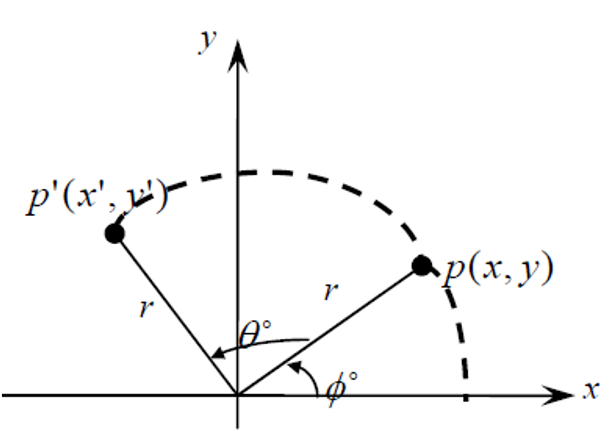
\includegraphics[width=0.29\textwidth]{figs/transf1.png}   
    \end{wrapfigure}
    \alert{证明:}
    $\left\{\begin{matrix}
        x'=x\cos\theta -y\sin\theta\\
        y'=x\sin\theta+y\cos\theta
    \end{matrix}\right.$ \qquad
    $\begin{bmatrix}
        x' \\
        y'
    \end{bmatrix}
    =
    \begin{bmatrix}
        \cos\theta & -\sin\theta\\
        \sin\theta & \cos\theta
    \end{bmatrix}
    \begin{bmatrix}
        x \\
        y
    \end{bmatrix}$\\
    $$ R_\theta=
    \begin{bmatrix}
        \cos\theta &-\sin\theta\\
        \sin\theta &\cos\theta
    \end{bmatrix} ,\qquad
    R_\theta ^{\dagger}=
    \begin{bmatrix}
        \cos\theta &\sin\theta\\
        -\sin\theta &\cos\theta
    \end{bmatrix} $$
    $$ R_\theta  R_\theta ^{\dagger} = R_\theta ^{\dagger} R_\theta=  
    \begin{bmatrix}
        \cos\theta &-\sin\theta\\
        \sin\theta &\cos\theta
    \end{bmatrix}
    \begin{bmatrix}
        \cos\theta &\sin\theta\\
        -\sin\theta &\cos\theta
    \end{bmatrix}
    =I
    $$
    证毕!
\end{frame}

\section{基矢变换}
\begin{frame} 
    \frametitle{}
    \begin{tcolorbox1}{1、基矢变换}
        试证明:量子力学不同表象基组之间的变换是幺正变换  
    \end{tcolorbox1}
    \alert{证明:} 设A的基组为$\psi_\alpha$ B的基组为 $\varphi_n$, A归一化公式中把波函数在B展开: 
    \begin{equation*}
        \begin{split}
            \delta_{\alpha\beta} &= (\psi_\alpha, \psi_\beta) \\
            &= (\sum_n S_{n\alpha} \varphi_n, \sum_m S_{m\beta} \varphi_m)\\
            &= \sum_{nm} S_{n\alpha} ^* S_{m\beta}(\varphi_n, \varphi_m)\\
            &= \sum_{nm} S_{n\alpha} ^* S_{m\beta}\delta_{nm}\\
            &= \sum_{n} S_{n\alpha} ^* S_{n\beta} = \sum_{n} S^{\dagger } _{\alpha n} S_{n\beta}
        \end{split} 
    \end{equation*}
\end{frame}

\begin{frame} 
    B归一化公式也可在A展开: 
    \begin{equation*}
        \begin{split}
            \sum_{\alpha} S_{n\alpha}  S^{\dagger } _{\alpha m}&=\sum_{\alpha} S_{n\alpha}  S_{m \alpha} ^* \\
            &=\sum_{\alpha} (\varphi_n, \psi_\alpha) (\varphi_m, \psi_\alpha)^* \\
            &=\sum_{\alpha} (\psi_\alpha,\varphi_n)^* (\psi_\alpha,\varphi_m) \\
            &=\sum_{\alpha\beta} (\psi_\alpha,\varphi_n)^* (\psi_\beta,\varphi_m) \delta_{\alpha\beta} \\
            &=\sum_{\alpha\beta} S_{\alpha n}^*  S_{\beta m} (\psi_\alpha,\psi_\beta)\\
            &= (\sum_{\alpha} S_{\alpha n}\psi_\alpha,\sum_{\beta} S_{\beta m}\psi_\beta)\\
            &= (\varphi_n,\varphi_m) =\delta_{nm} 
        \end{split} 
    \end{equation*}
\end{frame}

\begin{frame} 
    因此,我们有:
    \begin{equation*}
        \begin{split}
            \sum_{\alpha} S_{n\alpha}   S^{\dagger } _{\alpha m} &=\delta_{nm} \\
            \sum_{n} S^{\dagger } _{\alpha n} S_{n\beta}&=\delta_{\alpha\beta}
        \end{split} 
    \end{equation*}
    即:$$ S^{\dagger }S=SS^{\dagger } =I$$ 
    证毕! \\

    注意到: $ S_{n\alpha} = (e_n, e_\alpha)= (e_{(B)}, e_{(A)})$ \\
    得变换公式: $$ \color{red} u_{(B)}= S^{\dagger} u_ {(A)}$$
\end{frame}

\section{波函数变换}
\begin{frame} 
    \begin{tcolorbox1}{2、波函数变换}
        试证明:同一波函数在两不同表象中的矩阵之间的变换是幺正变换  
    \end{tcolorbox1}
    \alert{证明:} 设A的基组为$\psi_\alpha$ B的基组为 $\varphi_n$\\
    波函数$\Psi$在A表象和B表象中分别展开:
    \begin{equation*}
        \begin{split}
            \sum_\alpha a_\alpha \psi_\alpha &= \sum_n b_n \varphi_n \\
            \sum_\alpha a_\alpha \psi_\beta ^* \psi_\alpha &= \sum_n b_n \psi_\beta ^* \varphi_n \\
            \sum_\alpha a_\alpha (\psi_\beta, \psi_\alpha) &= \sum_n b_n (\psi_\beta, \varphi_n) \\
            \sum_\alpha a_\alpha \delta_{\alpha\beta} &= \sum_n b_n (\psi_\beta, \varphi_n) \\
            a_\alpha &= \sum_n S_{\alpha n} b_n\\
        \end{split} 
    \end{equation*}
\end{frame}

\begin{frame} 
    \begin{equation*}
        \begin{split}
            \Psi &= \\
            a_\alpha &= \sum_n S_{\alpha n} b_n\\
            a&=Sb\\
            \color{red} b& \color{red}=S^{\dagger}a   
        \end{split} 
    \end{equation*}
    正是两基组之间的幺正矩阵\\
    证毕!\\
\end{frame}

\section{算符变换}
\begin{frame} 
    \begin{tcolorbox1}{3、算符变换}
        试证明:同一力学量在两不同表象中的矩阵变换是幺正变换  
    \end{tcolorbox1}
    \alert{证明:} 设A的基组为$\psi_\alpha$ B的基组为 $\varphi_n$\\
    算符F在A表象的矩阵元为$F_{\alpha\beta}$, 在B表象中的矩阵元为$F'_{nm}$
    \begin{equation*}
        \begin{split}
            F'_{nm} &= (\varphi_n, F\varphi_m) \\
            &= (\sum_{\alpha} S_{\alpha n}\psi_\alpha, F \sum_{\beta} S_{\beta m}\psi_\beta)\\
            &= \sum_{\alpha\beta} S_{\alpha n} ^* (\psi_\alpha, F \psi_\beta) S_{\beta m}\\
            &= \sum_{\alpha\beta} S_{\alpha n} ^* F_{\alpha\beta} S_{\beta m}
        \end{split} 
    \end{equation*}
\end{frame}


\begin{frame} 
    \begin{equation*}
    \begin{split}
        F'_{nm} &= \sum_{\alpha\beta} S_{n\alpha } ^{\dagger} F_{\alpha\beta} S_{\beta m} \\
        &= (S^{\dagger} F S)_{nm}
    \end{split} 
    \end{equation*} 
    $$\color{red} F'= S^{\dagger} F S $$
\end{frame}

\section{幺正变换性质}

\begin{frame} 
    \begin{tcolorbox1}{幺正变换性质1:}
        试证明:幺正变换不改变算符的本征值 
    \end{tcolorbox1}
    \alert{证明:}
    算符F在A表象的矩阵为F,本征矢为a, 在B表象中的矩阵为F' 本征矢为b,有本征方程:
    \begin{equation*}
        \begin{split}
            Fa&=fa \qquad (1)\\
            F'b&=f'b\\
            S^{\dagger} F S S^{\dagger}a &=f'S^{\dagger}a\\
            S^{\dagger} F a &=f'S^{\dagger}a\\
            SS^{\dagger} F a &=f'SS^{\dagger}a\\
            F a &=f'a \qquad (2)\\
        \end{split} 
    \end{equation*} 
    比较(1)(2)式,有$f=f'$, 证毕!
\end{frame}    

\begin{frame} 
    \begin{tcolorbox1}{幺正变换性质2:}
        试证明:幺正变换不改变矩阵的迹
    \end{tcolorbox1}
    \alert{证明:} 矩阵A的对角元素之和称为矩阵A的迹,用$SP(A)$或$tr(A)$表示,则性质\\
    $$tr(AB)=tr(BA) $$
    \begin{equation*}
        \begin{split}
            tr(AB) &=\sum_i (AB)_{ii}\\
            &=\sum_{i} \sum_{j} (A_{ij} B_{ji}) \\
            &=\sum_{i} \sum_{j} (B_{ji} A_{ij}) \\
        \end{split} 
    \end{equation*} 
\end{frame}    


\begin{frame}     
    \begin{equation*}
        \begin{split}
            tr(AB) &=\sum_{j} \sum_{i} (B_{ji} A_{ij}) \\
            &=\sum_{j} (BA)_{jj} \\
            &=tr(BA)
        \end{split} 
    \end{equation*}

    \begin{equation*}
        \begin{split}
            F'&= S^{\dagger} F S \\
            tr(F')&=tr(S^{\dagger} F S)\\
            &=tr(SS^{\dagger}  F)\\
            &=tr(F)\\
        \end{split} 
    \end{equation*} 
    证毕!
\end{frame}    

\begin{frame} 
    \begin{tcolorbox1}{幺正变换性质3:}
        幺正变换不改变物理规律,已知在 x 表象中有基本对易关系$xp_x-p_x x =-\hbar$ 试求它在p表象中的形式,然后证明这种对易关系不随表象发生变化。
    \end{tcolorbox1}
    \alert{解:} (1)在p表象, $$ \hat{x}=i\hbar\dfrac{\partial}{\partial p_x}, \qquad \hat{p}_x=p_x $$
     对任意波函数 $\Psi(p_x)$
    \begin{equation*}
        \begin{split}
            \hat{x}\hat{p}_x\Psi &= i\hbar\dfrac{\partial}{\partial p_x} (p_x \Psi )\\
            &= i\hbar\Psi + p_xi\hbar\dfrac{\partial}{\partial p_x}\Psi \qquad (a)\\
        \end{split} 
    \end{equation*} 

\end{frame}  
\begin{frame} 
    $$\hat{p}_x\hat{x}\Psi = p_x(i\hbar\dfrac{\partial}{\partial p_x}\Psi) \qquad (b)$$
    (a)-(b)
    $$\hat{x}\hat{p}_x\Psi-\hat{p}_x\hat{x}=i\hbar\Psi$$
    $$\hat{x}\hat{p}_x-\hat{p}_x\hat{x}=i\hbar$$
    (2) 在Q表象,$$ x'= S^\dagger x S, \qquad p'_x= S^\dagger p_x S $$
    \begin{equation*}
        \begin{split}
        x'p'_x-p'_x x' &= S^\dagger x S S^\dagger p_x S - S^\dagger p_x S S^\dagger x S \\
        &= S^\dagger x p_x S - S^\dagger p_x x S \\
        &= S^\dagger (x p_x -  p_x x) S \\
        &= i\hbar S^\dagger S \\
        &= i\hbar \\
        \end{split} 
    \end{equation*} 
\end{frame}  
\begin{frame}
    \begin{tcolorbox2}{推论:}
       \begin{enumerate}
           \item 量子体系进行任一幺正变换不改变它的全部物理内容
           \item 两个量子体系,如果能用幺正变换联系起来,则它们在物理上是等价的
       \end{enumerate} 
    \end{tcolorbox2}
\end{frame}

\begin{frame}
    \begin{tcolorbox2}{构造S矩阵的方法}
        已知一个算符F在A表象中的矩阵如下,求F表象和A表象之间的幺正变换矩阵S
        $$ H=
        \begin{bmatrix}
            2\varepsilon  & 0 & \varepsilon\\
            0 & 2\varepsilon & 0 \\
            \varepsilon & 0 2\varepsilon\\
        \end{bmatrix} $$
     \end{tcolorbox2}

     \alert{解:} 如果知道 A表象的基 $\{\psi_\alpha \}$, F表象的基 $ \{\varphi_n \}$, 则可直接通过计算内积得到:
     $$ S_{n\alpha} =(\varphi_n, \psi_\alpha) $$
     现在中知道一个非对角矩阵H,我们可以能过解久期方程得到本征值和本征函数,得到一个对角阵H',这相当于实现了一个从A表象到H表象的幺正变换,关系式为:
     $$ H'=S^\dagger H S$$
     上式H和H'已知,因此S可求。 
\end{frame}  

\begin{frame}
现在证明:F在A表象的本征函数系构成这个S矩阵。\\
\alert{证明:} 注意到H'的对角元是本征值
\begin{equation*}
    \begin{split}
    H' &=S^\dagger H S \\
    H'_{mn} &=(S^\dagger H S)_{mn}  \\
    \sum_{\alpha \beta} S^{\dagger} _{m \alpha} H_{\alpha \beta} S_{\beta n} & = h_m \delta_{mn} \\
    \sum_{\alpha \beta} (\sum_m S_{\alpha m} S^\dagger_{m \alpha}) H_{\alpha \beta} S_{\beta n} &= h_m \sum_m S_{\alpha m}\delta_{mn} \\
    \sum_{\beta} H_{\alpha \beta} S_{\beta n} &= h_n S_{\alpha n} \\
    \end{split} 
\end{equation*} 
上式表明,第n个本征态正好是S矩阵的第n列!\\
即依次提列本征函数构成S阵。证毕!
\end{frame} 

\begin{frame}
    THE END
\end{frame}  


 



  %   
%%%%%%%%%%%%%%%%%%%%%%%%%%%%%%%%%%%%55%%
\begin{frame} [plain]
    \frametitle{}
    \Background[1] 
    \begin{center}
    { {\huge 第十五讲、狄拉克(Dirac)符号}}
    \end{center}  
    \addtocounter{framenumber}{-1}   
\end{frame}
%%%%%%%%%%%%%%%%%%%%%%%%%%%%%%%%%%

%%%%%%%%%%%%%%%%%%%%%%%%%%%%%%%%%
\begin{frame}
        \frametitle{主要内容}
        \transfade
        \tableofcontents
        \addtocounter{framenumber}{-1} 
\end{frame}
%%%%%%%%%%%%%%%%%%%%%%%%%%%%%%%%%%

\section{前情回顾}

\begin{frame}
    \frametitle{前情回顾}
    \begin{itemize}
       \done 波动力学
       \done 矩阵力学
       \todo 两者的统一 
    \end{itemize}
        \begin{center}
            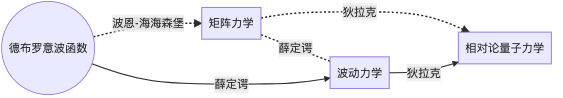
\includegraphics[width=0.9\textwidth]{figs/2021-12-06-16-22-39.png}\\   
        \end{center}    
\end{frame} 

\section{狄拉克(Dirac)符号}

\begin{frame}
    量子力学用希尔伯特空间描述,希尔伯特空间是内积空间
    \begin{tcolorbox1}{希尔伯特空间}
    \begin{itemize}
        \item 加法:$\psi + \varphi$
        \item 数乘:$c\psi$
        \item 内积:$(\psi,\psi)$
    \end{itemize}
    \end{tcolorbox1}
    考察内积: $(\psi,\psi)=\int\psi^*\psi d\tau$ \\
    同一波函数放在左边还是右边,意义有所不同: \\
    放右边是线性矢量:  $(\psi,a\psi)=a (\psi,\psi)$ \\
    放左边是反线性矢量:   $(a\psi,\psi)=a^* (\psi,\psi)$   
\end{frame}

\begin{frame}
    \frametitle{1、左矢和右矢}
    \begin{tcolorbox1}{定义:}
    为了清楚地描述这种线性反线性特点,特定义左矢和右矢
    $$\langle \psi |, \qquad |\psi \rangle $$ 
    内积:\[(\psi,\psi)\equiv \langle \psi | \psi \rangle\]

    有性质: $$\langle a\psi | = \langle \psi |a^* $$
    $$ |a\psi \rangle = a|\psi \rangle$$ 
    \end{tcolorbox1}
\end{frame} 

\begin{frame}
    \frametitle{}
    考察加法和数乘:发现其中的矢量通常是线性的,因此用右矢来代替。\\
    $$\begin{aligned}
    &\text{内积:}   & (\psi,\Psi)  & \qquad\Leftrightarrow \qquad & | \Psi \rangle =\langle \psi | \Psi \rangle \\
    &\text{平均值:}   & \bar{F}=(\Psi,F\Psi)  & \qquad\Leftrightarrow \qquad & \bar{F} =\langle \Psi|F | \Psi \rangle \\
    &\text{态叠加原理:}   & \Psi=a_1 \psi_1+ a_2 \psi_2  & \qquad\Leftrightarrow \qquad &| \Psi \rangle =a_1 |1 \rangle+ a_2 |2 \rangle\\
    &\text{展开式1:}     & \Psi=\sum\limits_{i=1} ^n a_i \psi_i & \qquad \Leftrightarrow \qquad &| \Psi \rangle =\sum\limits_{i=1} ^n a_i |i \rangle\\
    &\text{展开式2:}     & \Psi=\sum\limits_{i=1} ^n (\psi_i ,\Psi) \psi_i & \qquad \Leftrightarrow \qquad &| \Psi \rangle =\sum\limits_{i=1} ^n \langle i | \Psi \rangle |i\rangle\\
    \end{aligned}
    $$
\end{frame} 
 

\begin{frame}
    \frametitle{2、外积}
    考察展开式:
    $$\begin{aligned}
    \Psi \rangle &= \sum\limits_{i=1} ^n \langle i | \Psi \rangle |i\rangle\\
                 &= \sum\limits_{i=1} ^n |i\rangle\langle i | \Psi \rangle \\
    \end{aligned}
    $$
    定义算符: $ \qquad  \rho_i = |i\rangle\langle i | \qquad $ 有: \\
    $$\sum\limits_{i=1} ^n |i\rangle\langle i = \sum\limits_{i=1} ^n \rho_i =1 $$

\end{frame} 

\begin{frame}
    \frametitle{外积矩阵表示}
    若:$ \Psi =\sum a_n \varphi_n $\\
    右矢的矩阵形式:
    $$|\Psi\rangle = \begin{pmatrix}
        a_1\\
        a_2\\\
        \cdots\\
        a_n\
    \end{pmatrix}$$ 
    左矢的矩阵形式:
    $$ \langle\Psi| = (a_1 ^*, a_2 ^*, \cdots, a_n ^*) $$
    内积与外积:
    $$\langle\Psi|\Psi\rangle= (a_1 ^*, a_2 ^*, \cdots, a_n ^*) \begin{pmatrix}
        a_1\\
        a_2\\\
        \cdots\\
        a_n\
    \end{pmatrix},\qquad  |\Psi\rangle\langle\Psi|= \begin{pmatrix}
        a_1\\
        a_2\\\
        \cdots\\
        a_n\
    \end{pmatrix} (a_1 ^*, a_2 ^*, \cdots, a_n ^*) $$
\end{frame} 


\begin{frame}
    \frametitle{3、密度算符}
    算符的意义:
    $$\rho_i\Psi= |i\rangle\langle i | \Psi \rangle = \langle i | \Psi \rangle |i\rangle=a_i |i\rangle $$
    $$\Psi= \sum\limits_i ^n a_i |i\rangle = \sum\limits_i ^n \rho_i\Psi$$
    可知: $ \rho_i\Psi $ 是矢量$\Psi$ 在第$i$ 个本征矢上的投影, 因此称为{\color{red} 投影算符}\\
    对于非本征态,也可定义:$\rho = |\Psi\rangle\langle \Psi |$\\
    考察其在$i$态的平均值:
    $$ \begin{aligned}
    \bar{\rho} &=\langle i |\rho | i \rangle \\
               &=\langle i |\Psi\rangle\langle \Psi | i \rangle \\
               &=(\langle i |\Psi\rangle) (\langle \Psi | i \rangle) \\
               &=a_i ^* a_i =\omega_i \\
    \end{aligned} $$
    是概率密度,因此称 $\rho = |\Psi\rangle\langle \Psi |$ 为 {\color{red} 密度算符},也称为测量算符。
\end{frame} 
 
\begin{frame}
    \frametitle{4、密度矩阵}
    考察平均值公式:\\
    $$ \begin{aligned}
    \bar{\hat{F}} &=\sum\limits_i |a_i|^2 f_i \\
            &=\sum\limits_i \omega_i \langle i |\hat{F}|i \rangle  \\
            &=\sum\limits_{ij} \omega_i \langle i |\hat{F} |j\rangle \langle j| i\rangle  \\
            &=\sum\limits_{ij} \langle j| i\rangle  \omega_i \langle i |\hat{F} |j\rangle  \\
            &=\sum\limits_{j} \langle j | (\sum\limits_{i}| i \rangle  \omega_i \langle i |) \hat{F} |j\rangle  \\
    \end{aligned} $$
    定义密度矩阵:$ \hat{\rho} = \sum\limits_{i}| i \rangle  \omega_i \langle i | $
\end{frame} 
 
\begin{frame}  
    \frametitle{}  得新的平均值公式:
    \begin{tcolorbox1}{平均值公式-3}
         $$ \begin{aligned}
            \bar{\hat{F}}&=\sum\limits_{j} \langle j | \hat{\rho} \hat{F} |j\rangle \\
                &=tr (\hat{\rho} \hat{F} )
        \end{aligned} $$   
    \end{tcolorbox1} 
\end{frame} 
 
\begin{frame}      
    例:求算符$\hat{F}$在 $|\Psi\rangle =\sum\limits_n a_n |n\rangle $上的平均值 \\
    \alert{解:} 先求算符矩阵:
    $$ F_{nm} = \langle n | F |m \rangle  $$
    再求密度矩阵:
    $$ \hat{\rho} = \sum\limits_{n}| n \rangle  a_n ^* a_n \langle n | $$
    对两矩阵的积求迹得平均值
    $$\bar{\hat{F}}=tr (\hat{\rho} \hat{F} )$$
\end{frame} 
 
\begin{frame}  
    \frametitle{6、狄拉克型量子力学}  
    量子态: $\hspace{1em}|\Psi \rangle, \qquad$ 位置波函数:$\hspace{1em} \langle x |\Psi \rangle$ \\ \vspace{0.2em}
    展开式: $\hspace{1em}|\Psi \rangle =\sum\limits_{n=1} ^n a_n |n \rangle$ \\
    内积:   $\hspace{2em}\langle \varphi | \Psi \rangle = (\varphi, \Psi)= \int \varphi^*\Psi d\tau $ \\  \vspace{0.2em}
    归一化: $\hspace{1em}\langle \Psi | \Psi \rangle = (\Psi, \Psi)= \int \Psi^*\Psi d\tau = 1 $ \\ \vspace{0.2em}
    正交归一: $\langle n | m \rangle = \delta_{nm} $ \\ \vspace{0.2em}
    $ \hspace{5em} \langle \lambda | \lambda' \rangle = \delta(\lambda-\lambda') $\\ \vspace{0.2em}
    表象: $\hspace{2em}\Psi(x)= \langle x | \Psi \rangle$ \\ \vspace{0.2em}
    展开系数: $ a_n= \langle n | \Psi \rangle$ \\ \vspace{0.2em}
    展开系数: $ a_n ^*= \langle \Psi | n \rangle$ \\ \vspace{0.2em}
    平均值:  $\hspace{1em}\bar{F} = \langle \Psi |F | \Psi \rangle$ \\ \vspace{0.2em}
\end{frame} 
 
\begin{frame} 
    矩阵元:  $\hspace{1em}F_{nm} = \langle n |F | m \rangle$ \\ \vspace{0.2em}
    本征方程:$F|n\rangle =f_n |n\rangle$ \\ \vspace{0.2em}
    幺正变换:$S_{m\alpha} =\langle m| \alpha \rangle $ \\ \vspace{0.2em}
    密度算符:$\rho = |\Psi\rangle\langle \Psi | $ \\ \vspace{0.2em}
    密度矩阵: $\hat{\rho} = \sum\limits_{i}| i \rangle  \omega_i \langle i | $ \\ \vspace{0.2em}
    薛定谔方程:$$ i\hbar \frac{\partial }{\partial t} |\Psi(t)\rangle = H|\Psi(t)\rangle $$ 
    算符运动方程:$$ \frac{d\bar{A}(t)}{dt}=\overline{(\frac{\partial A(t) }{\partial t})}  +\frac{1}{i\hbar} \overline{[A(t),H(t)]}$$
\end{frame} 
 
\begin{frame} 
    \frametitle{8、应用实例}  
    1、求波函数的矩阵表示:  
    $$|\Psi \rangle =\sum\limits_{n=1} ^n a_n |n \rangle$$
    $$ a_n= \langle n | \Psi \rangle$$ 
    展开系数构成矩阵表示:  
    $$\begin{pmatrix}
    a_1\\
    a_2\\\
    \cdots\\
    a_n\
    \end{pmatrix} $$
\end{frame} 

\begin{frame} 
    \frametitle{}  
    2、求算符的矩阵表示:  
    $$|\varphi \rangle = F |\Psi \rangle$$
    $$|\varphi \rangle = \sum_n F |n\rangle\langle n |\Psi \rangle$$
    $$\langle m |\varphi \rangle = \sum_n  \langle m| F |n\rangle\langle n |\Psi \rangle$$
    $$ b_m = \sum_n  F_{mn} a_n$$

    取遍$n,m$:  
    $$\begin{pmatrix}
    b_1\\
    b_2\\\
    \cdots\\
    b_n\
    \end{pmatrix} 
    = 
    \begin{pmatrix}
        F_{11} & F_{12} & \cdots & F_{1n} \\
        F_{21} & F_{22} & \cdots & F_{2n} \\
        \cdots & \cdots &  \cdots &  \cdots \\
        F_{n1} & F_{n2} & \cdots & F_{nn} \\
    \end{pmatrix} 
    \begin{pmatrix}
        a_1\\
        a_2\\\
        \cdots\\
        a_n\
    \end{pmatrix} 
    $$
\end{frame} 

\begin{frame} 
    3、求薛定谔方程的矩阵表示: 
    $$ \begin{aligned}
    i \hbar \frac{\partial}{\partial t} |\Psi \rangle &= H |\Psi \rangle  \\
    i \hbar \frac{\partial}{\partial t} \langle m |\Psi \rangle &= \langle m |H |\Psi \rangle \\ 
     &= \sum_n \langle m |H |n\rangle\langle n |\Psi \rangle  \\
     i \hbar \frac{\partial}{\partial t} a_m  &= \sum_n H_{mn} a_n 
    \end{aligned}
    $$
\end{frame} 

\begin{frame} 
    4、求平均值公式的矩阵表示: 
    $$ \begin{aligned}
    \bar{F} &= \langle \Psi |F |\Psi \rangle  \\
    &= \langle \Psi |1 \cdot F \cdot 1 |\Psi \rangle  \\
    &= \sum_{mn} \langle \Psi |m\rangle\langle m |F| n\rangle\langle n |\Psi \rangle  \\
    &= \sum_{mn} a_m ^* F_{mn} a_n 
    \end{aligned}
    $$
\end{frame} 

\begin{frame} 
    5、求两算符积的平均值: 
    $$ \begin{aligned}
    \overline{GF} &= \langle \Psi |GF |\Psi \rangle  \\
    &= \langle \Psi |1 \cdot G \cdot 1 \cdot F \cdot 1 |\Psi \rangle  \\
    &= \sum_{mln} \langle \Psi |m\rangle\langle m |G |l\rangle\langle l| F| n\rangle\langle n |\Psi \rangle  \\
    &= \sum_{mln} a_m ^* G_{ml} F_{ln} a_n 
    \end{aligned}
    $$
\end{frame} 

\section{量子力学绘景(Pictures)}

\begin{frame}  
    \frametitle{三种绘景}
    量子力学二个基本方程:  
    \begin{enumerate}
        \item 薛定谔方程:$$ i\hbar \frac{\partial }{\partial t} |\Psi(t)\rangle = H|\Psi(t)\rangle $$
        \item 算符运动方程:$$ \frac{d\bar{A}(t)}{dt}=\overline{(\frac{\partial A(t) }{\partial t})}  +\frac{1}{i\hbar} \overline{[A(t),H(t)]}$$
    \end{enumerate}
    这个世界到底什么在变?\\
    \begin{itemize}
        \done 薛定谔绘景:只有波函数(态)在变,服从薛定谔方程
        \done 海森堡绘景:只有算符(力学量)在变,服从算符运动方程(海森堡方程)
        \done 狄拉克绘景:波函数和算符都在变,一切都只是幺正变换。
    \end{itemize}
\end{frame} 

\begin{frame}  
    \frametitle{}  
    定义时间演化算符:
    $$ U(t,t_0) |\Psi(t_0)\rangle = |\Psi(t)\rangle  $$
    \alert{分析}:
    (1) 因为 $ U(t_0,t_0) |\Psi(t_0)\rangle = |\Psi(t_0)\rangle  $ \\
     有:$$ U(t_0,t_0)=I $$
    (2):求 $ U(t,t_0)$
    $$ \begin{aligned}
        i\hbar \frac{\partial }{\partial t} |\Psi(t)\rangle &= H|\Psi(t)\rangle  \\
        i\hbar \frac{\partial }{\partial t}  U(t,t_0) |\Psi(t)\rangle &= H U(t,t_0) |\Psi(t)\rangle  \\
        i\hbar \frac{\partial }{\partial t}  U(t,t_0)  &= H U(t,t_0)  \\
        U(t,t_0)  &= e^{-\frac{i}{\hbar} H(t-t_0)}  \\
    \end{aligned} $$
\end{frame} 

\begin{frame}  
    (3):$ U(t,t_0)$是幺正算符
    $$ \begin{aligned}
        U(t,t_0)  &= e^{-\frac{i}{\hbar} H(t-t_0)}  \\
        U^\dagger (t,t_0)  &= e^{\frac{i}{\hbar} H(t-t_0)}  \\
        U^\dagger (t,t_0)U(t,t_0) &= U^\dagger (t,t_0)U(t,t_0) \\
         &=e^{\frac{i}{\hbar} H(t-t_0)-\frac{i}{\hbar} H(t-t_0)} \\
         &=e^0
         &=I
    \end{aligned} $$
    因此,有:
    $$ |\Psi(t)\rangle = U(t,t_0) |\Psi(t_0)\rangle   $$
    对比: 
    $$ |\psi_{(B)}\rangle = S^\dagger |\psi_{(A)}\rangle $$
    可知,波函数随时间的演化服从薛定谔方程,但也只是一种幺正算符。
\end{frame} 

\begin{frame}  
    \frametitle{} 
    (4)分析平均值公式:
    $$ \begin{aligned}
        \bar{F} &= \langle \Psi(t) |F(t_0) | \Psi \rangle(t)  \\
        &= \langle \Psi(t_0) |U^\dagger (t,t_0) |F(t_0) | U(t,t_0) |\Psi(t_0)\rangle   \\
        &= \langle \Psi(t_0) |U^\dagger (t,t_0) F(t_0) U(t,t_0) |\Psi(t_0)\rangle   \\
        &= \langle \Psi(t_0) F(t,t_0) |\Psi(t_0)\rangle   \\
    \end{aligned} $$
     式中,令: $$ F(t,t_0) =U^\dagger (t,t_0) F(t_0) U(t,t_0)$$
     对式:
     $$F'=S^\dagger F S $$
     可知,算符随时间的演化与波函数随时间的演化是等价的,也只是一种幺正算符。
\end{frame} 

\begin{frame}
    \frametitle{}  
    \centering
    \LARGE \color{red} 期中考试! \\
\end{frame}  %  
%-----------------------------------------------%

%%%%%%%%%%%%%%%%%%%%%%%%%%%%%%%%%%%%%%%%%%%%%%%%%
\begin{frame}
	\begin{center}
		\huge Thanks for your attention! \\ \vspace{1.0em}
         A \& Q
	\end{center}
\end{frame}

%%%%%%%%%%%%%%%%%%%%%%%%%%%%%%%%%%%%%%%%%%%%%%%%%

\end{document}
